\chapter{Evaluation}
\label{chap:evaluation}

In this chapter, we discuss the results in the following four sections.
First, we go over the performance of the \gls{ocr} algorithms for each distortion type.
Then we compare the performance of the \gls{ocr} algorithms against human judgment.
Third, we investigate the feasibility of using recognized text from pristine images as ground truth.
Finally, we evaluate the performance of the \gls{ocr} algorithms on different quality levels of the HM and VTM codecs.

\section{Performance of Optical Character Recognition}
\label{sec:ocr_performance}

First, we assessed the impact of different distortion types on \gls{ocr} performance by comparing the mean $\text{CER}_{\text{c}}$ for various quality levels.
We performed this analysis separately for EasyOCR and Tesseract \gls{ocr} to determine which performs better.
For the comparison, we plotted the mean $\text{CER}_{c}$ with regards to the \gls{gt} on the y-axis against different quality levels on the x-axis.
We did this for all nine distortion types.

\begin{figure}[h]
\centering
    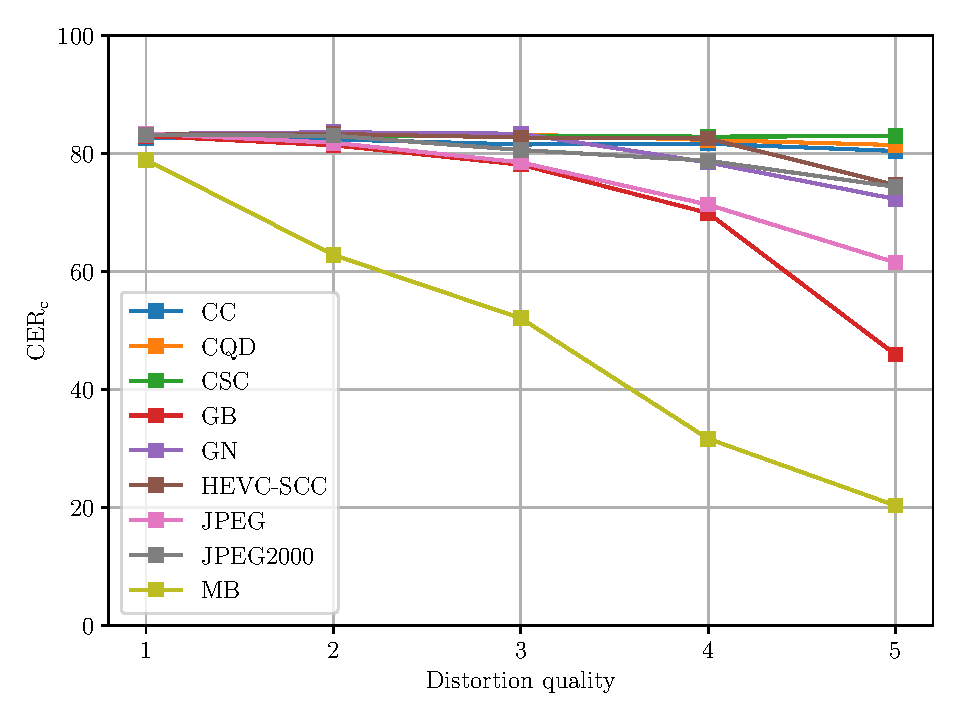
\includegraphics[width=\textwidth]{../../images/analyze/cer_dist_quality_gt_ezocr.pdf}
    \caption{Mean $\text{CER}_{\text{c}}$ in relation to the \gls{gt} for different quality levels with EasyOCR.}
\label{fig:cer_dist_quality_gt_ezocr}
\end{figure}

In \autoref{fig:cer_dist_quality_gt_ezocr}, we observe the mean $\text{CER}_{\text{c}}$ in relation to the \gls{gt} for different quality levels using EasyOCR.
We notice a trend that \gls{mb} has the most significant impact on EasyOCR's performance, exhibiting a nearly linear decrease from 80 to 20.
For \gls{jpeg} and \gls{gb} EasyOCR displays similar behavior until quality level 4, after which it experiences a steeper decline for \gls{gb}.
This may be due to the blurring of images greatly affecting the legibility of text, with letters becoming indistinct and merging together.
For \gls{gn}, \gls{jpeg2000} and \gls{hevcscc} EasyOCR exhibits comparable performance, experiencing a slight decline at quality level 5.
The remaining distortions have minimal impact on performance, which we expected since color distortions do not directly affect text shapes.

\begin{figure}[h]
\centering
    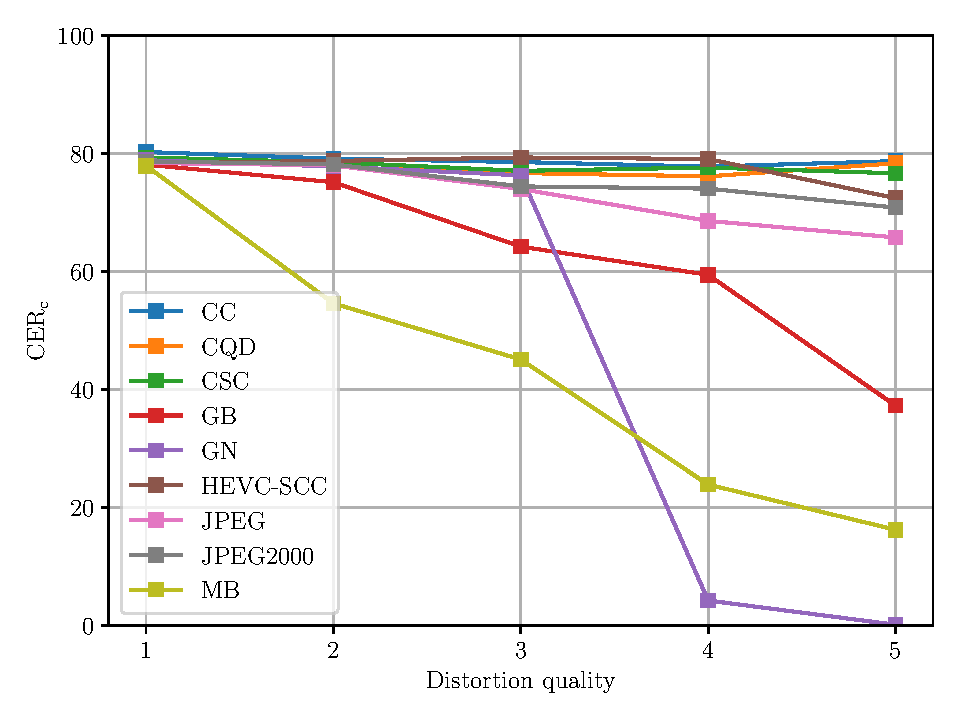
\includegraphics[width=\textwidth]{../../images/analyze/cer_dist_quality_gt_tess.pdf}
    \caption{Mean $\text{CER}_{\text{c}}$ in relation to the \gls{gt} for different quality levels with Tesseract \gls{ocr}.}
\label{fig:cer_dist_quality_gt_tesseract}
\end{figure}

In \autoref{fig:cer_dist_quality_gt_tesseract}, we can see the same analysis for Tesseract \gls{ocr}.
We see a steady decrease in $\text{CER}_{\text{c}}$ for \gls{mb} and \gls{gb}, with the former exhibiting a steeper decline.
However, the most noteworthy finding is the significant drop in $\text{CER}_{\text{c}}$ for \gls{gn} at quality level 4, reaching 0 at quality level 5.
This sudden decline is particularly surprising when compared to other types of distortions.
Among the distortions analyzed, \gls{cc}, \gls{cqd}, and \gls{csc}, with \gls{cc} even demonstrating a slightly higher $\text{CER}_{\text{c}}$ at quality level 5 compared to previous levels.
This phenomenon can possibly be attributed to \gls{cc}'s ability to enhance the distinction between the text and the background, acting almost like an image preprocessing step for the \gls{ocr}.
Interestingly, the $\text{CER}_{\text{c}}$ for \gls{hevcscc} slightly increases at quality level 4 and then decreases again at quality level 5.
A plausible explanation for this behavior is that certain portions of the text are not well recognized at quality 4, and since these unrecognized parts are not included in the \gls{gt}, it leads to a higher $\text{CER}_{\text{c}}$.
At level 5, more text elements, that are in the ground truth, are not recognized well and overshadow the earlier phenomenon.
Consequently, the $\text{CER}_{\text{c}}$ decreases.

In summary, our observations reveal that \gls{mb} and \gls{gb} have a substantial impact on the performance of both EasyOCR and Tesseract \gls{ocr} algorithms.
Additionally, both \gls{ocr} algorithms demonstrate superior performance across images with \gls{cc}, \gls{cqd}, and \gls{csc}.
However, the most remarkable discovery is the significant drop in the $\text{CER}_{\text{c}}$ for Gaussian noise at quality level 4, reaching 0 at quality level 5, specifically for Tesseract OCR.
This suggests that EasyOCR exhibits greater robustness to \gls{gn} compared to Tesseract \gls{ocr} .
Overall, EasyOCR outperforms Tesseract \gls{ocr}, with a performance ceiling of approximately 83 $\text{CER}_{\text{c}}$ for EasyOCR, while Tesseract \gls{ocr} only achieves around 70 $\text{CER}_{\text{c}}$.

\section{Comparison Against Human Judgment}
\label{sec:comparison_against_human_judgment}

In this section, we compare the performance of the \gls{ocr} algorithms with human judgment.
We use the subjective quality scores to investigate the correlation between the $\text{CER}_{\text{c}}$ and the \gls{mos}.
However, compared to the last section, we calculate the $\text{CER}_{\text{c}}$ in relation to the reference image instead of the ground truth.
This makes it a fairer comparison as the humans that rated the images, compared the distorted images to the reference image to arrive at the \gls{mos}.


% mos vs cer mean in relation to reference for easyocr
\begin{figure}[h]
\centering
    \begin{subfigure}[b]{0.3\textwidth}
        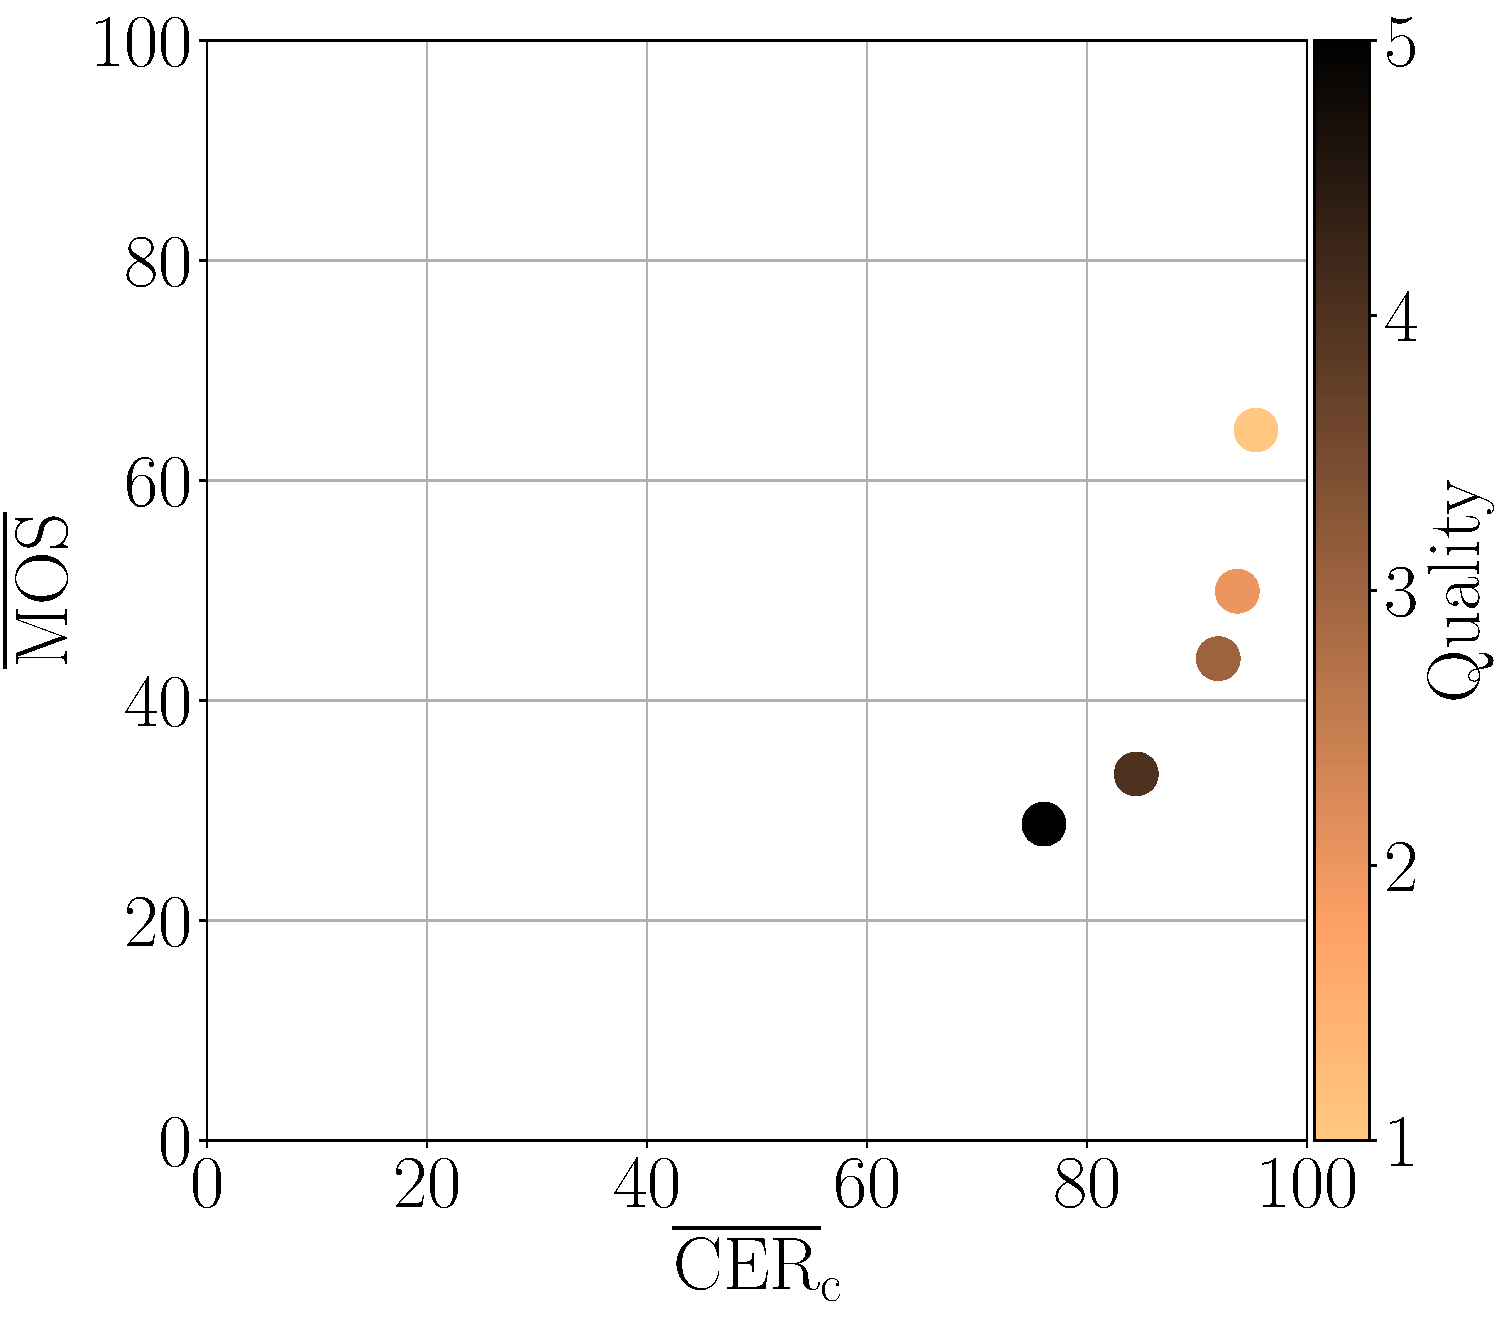
\includegraphics[width=\textwidth]{../../images/analyze/mos_cer_ref_mean_ezocr_GN.pdf}
        \caption{GN}
        \label{fig:mos_cer_ref_mean_ezocr_GN}
    \end{subfigure}
    \hfill
    \begin{subfigure}[b]{0.3\textwidth}
        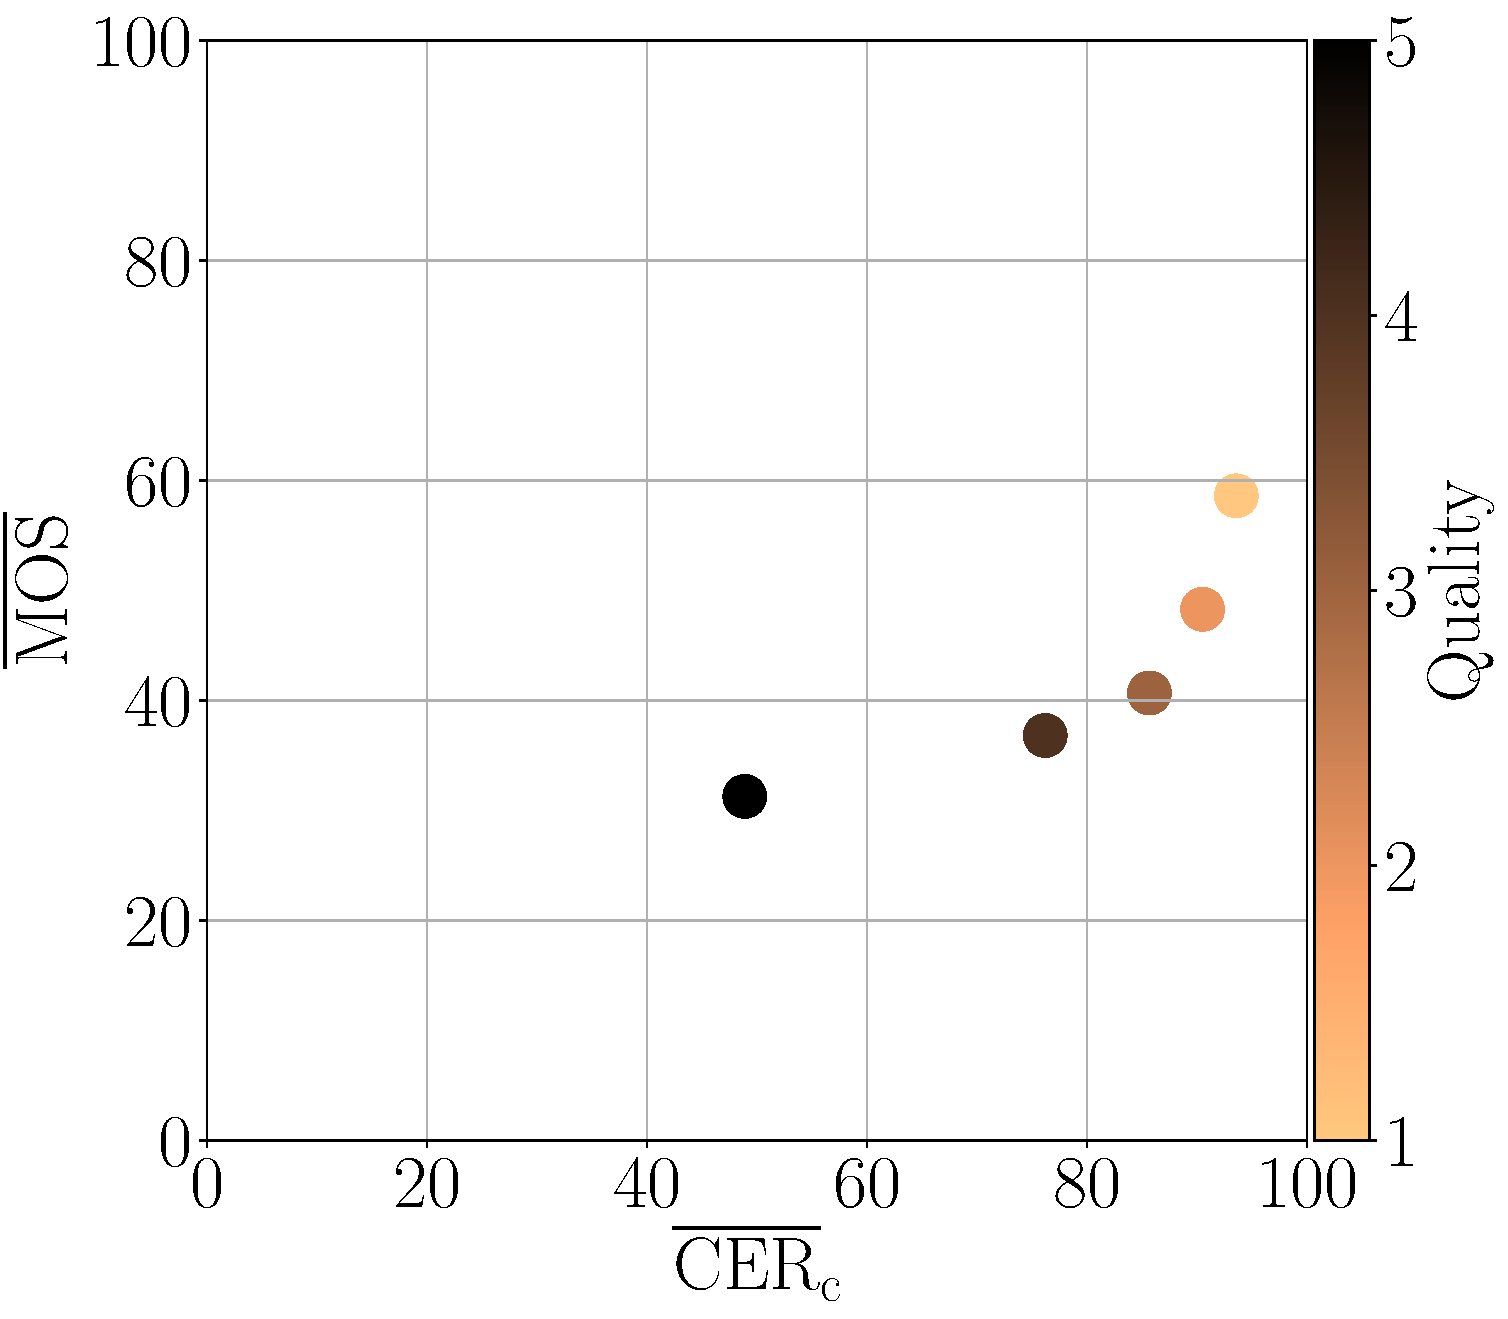
\includegraphics[width=\textwidth]{../../images/analyze/mos_cer_ref_mean_ezocr_GB.pdf}
        \caption{GB}
        \label{fig:mos_cer_ref_mean_ezocr_GB}
    \end{subfigure}
    \hfill
    \begin{subfigure}[b]{0.3\textwidth}
        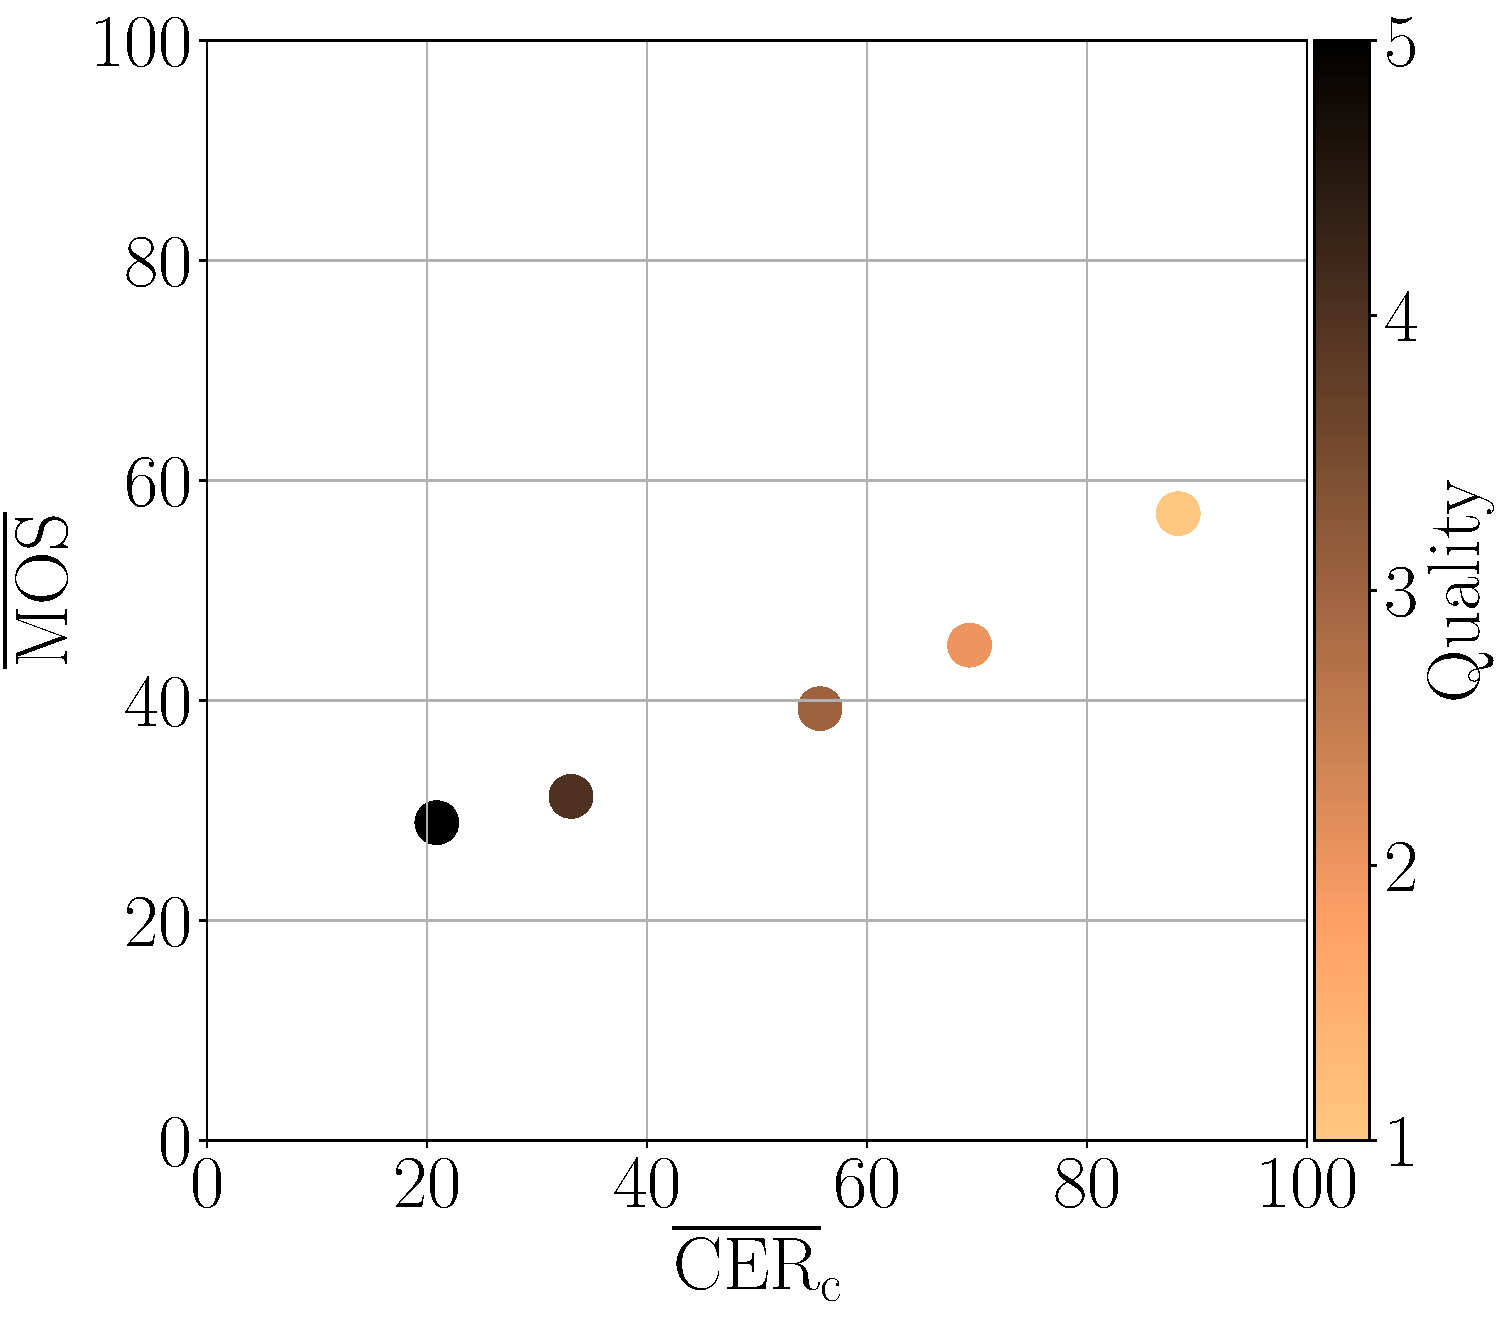
\includegraphics[width=\textwidth]{../../images/analyze/mos_cer_ref_mean_ezocr_MB.pdf}
        \caption{MB}
        \label{fig:mos_cer_ref_mean_ezocr_MB}
    \end{subfigure}
    \newline
    \begin{subfigure}[b]{0.3\textwidth}
        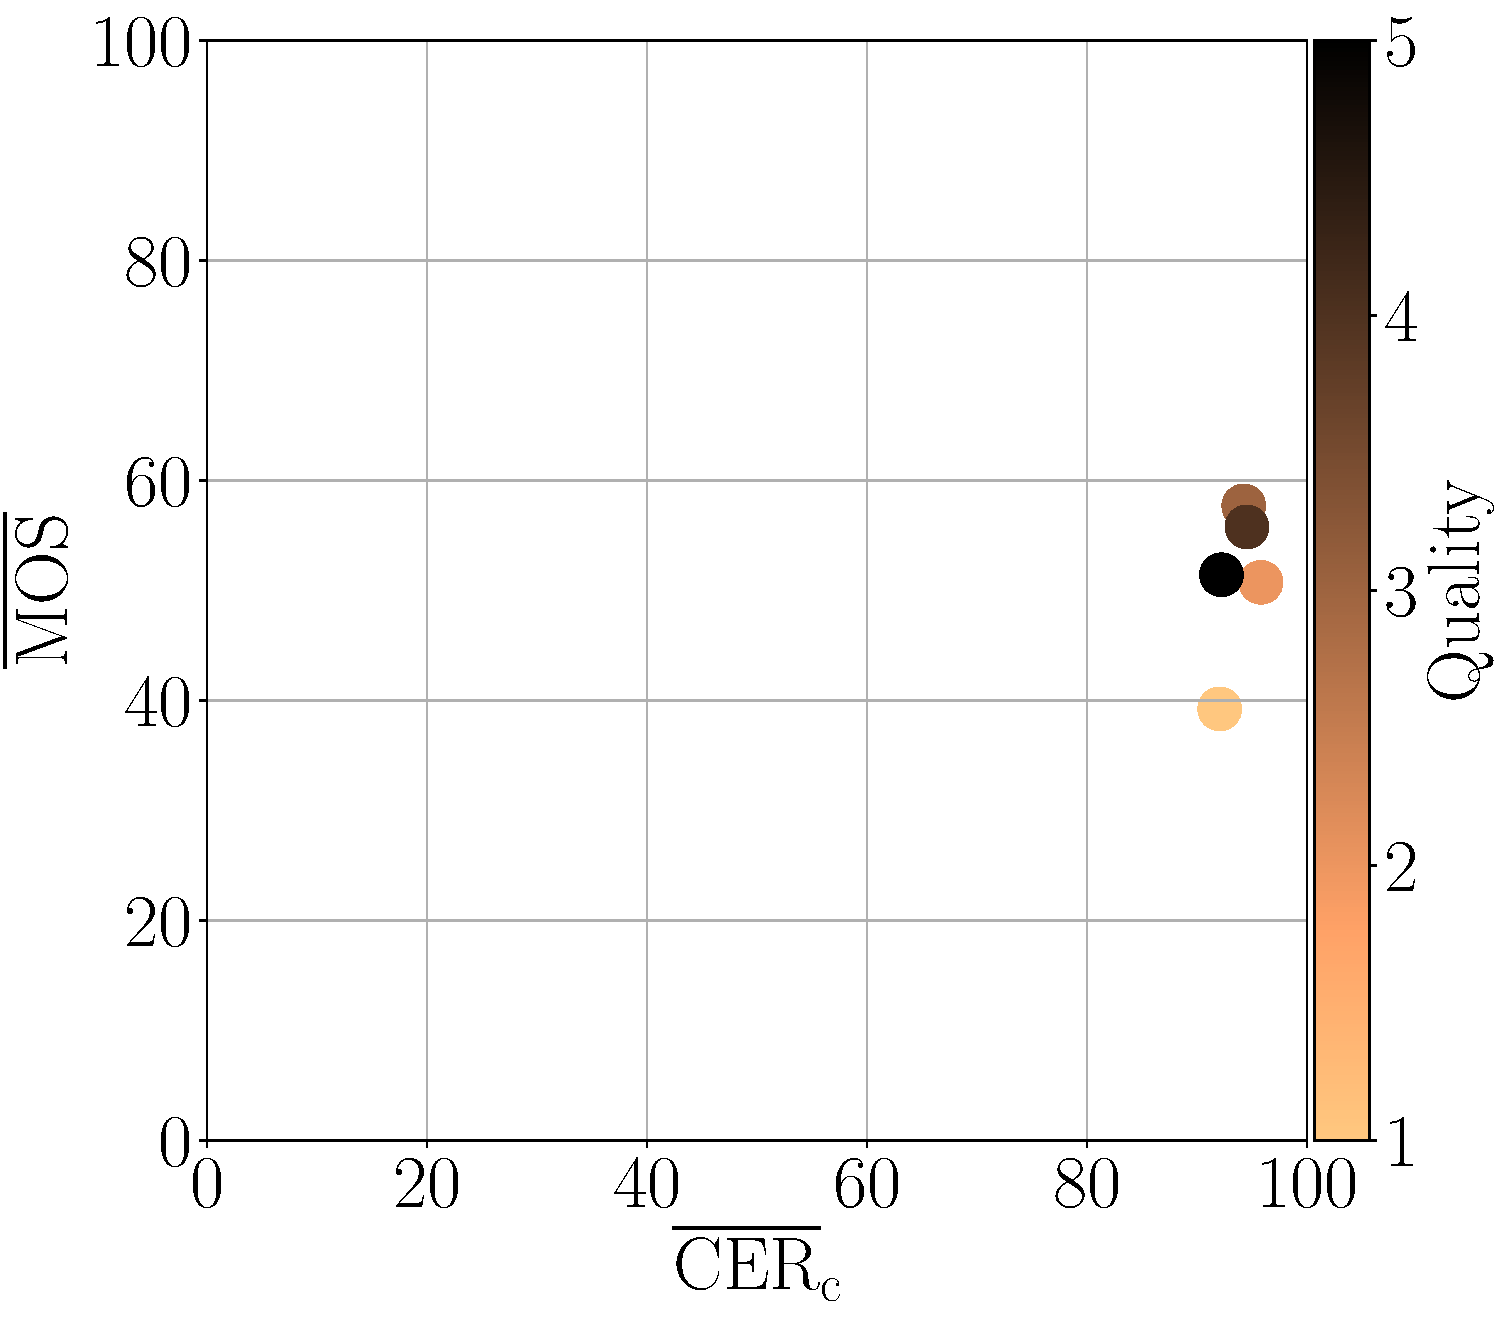
\includegraphics[width=\textwidth]{../../images/analyze/mos_cer_ref_mean_ezocr_CC.pdf}
        \caption{CC}
        \label{fig:mos_cer_ref_mean_ezocr_CC}
    \end{subfigure}
    \hfill
    \begin{subfigure}[b]{0.3\textwidth}
        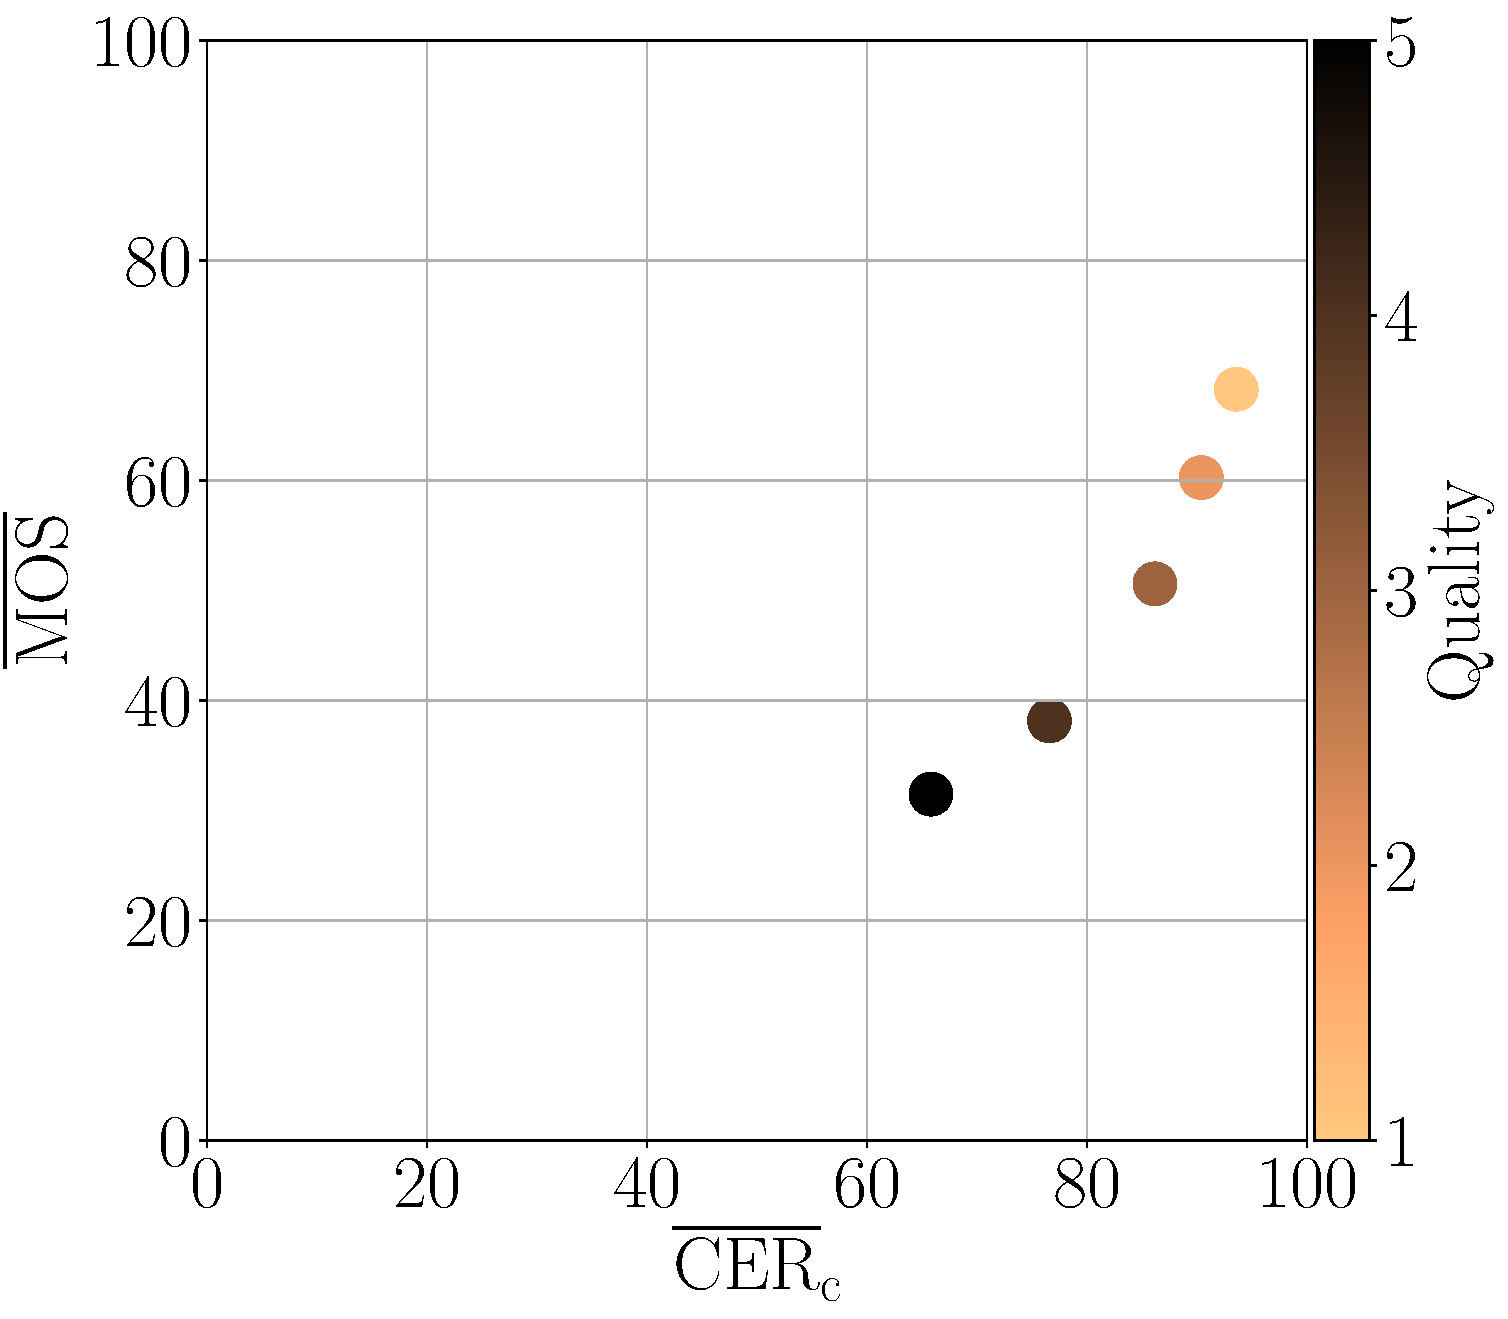
\includegraphics[width=\textwidth]{../../images/analyze/mos_cer_ref_mean_ezocr_JPEG.pdf}
        \caption{JPEG}
        \label{fig:mos_cer_ref_mean_ezocr_JPEG}
    \end{subfigure}
    \hfill
    \begin{subfigure}[b]{0.3\textwidth}
        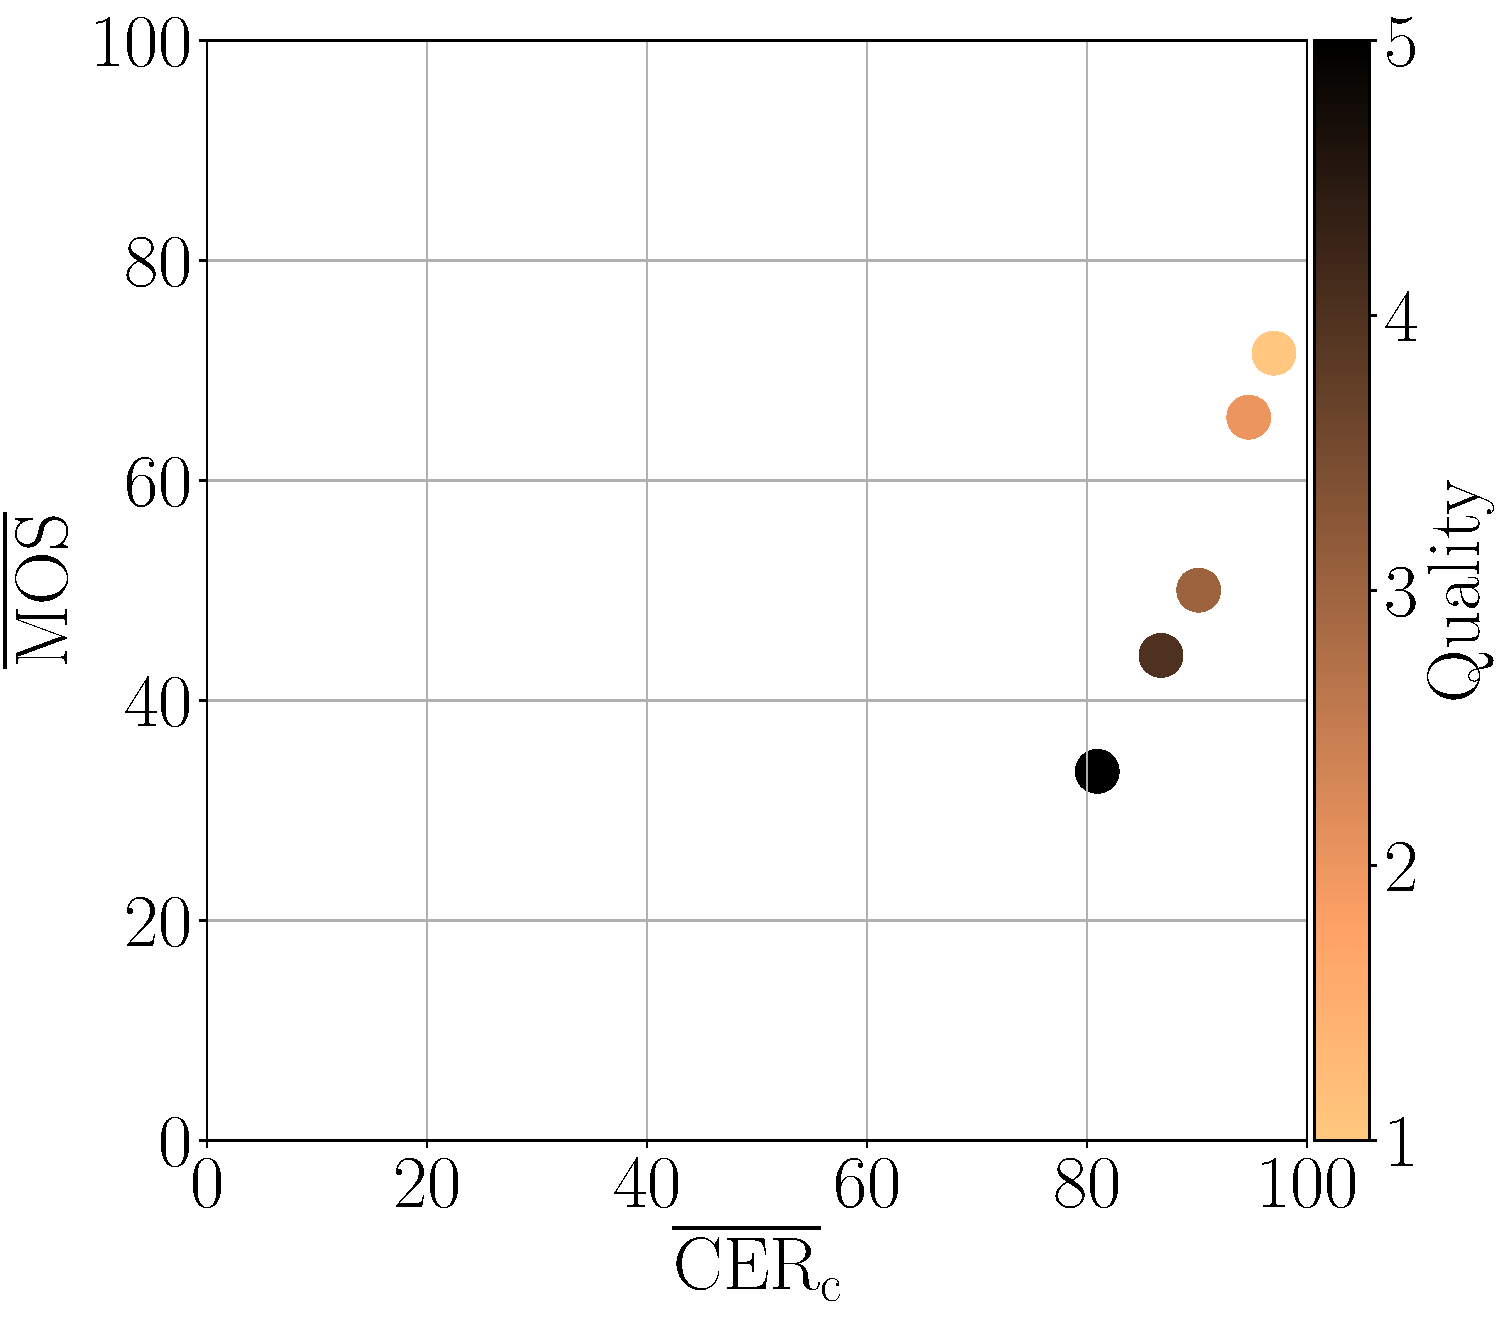
\includegraphics[width=\textwidth]{../../images/analyze/mos_cer_ref_mean_ezocr_JPEG2000.pdf}
        \caption{JPEG2000}
        \label{fig:mos_cer_ref_mean_ezocr_JPEG2000}
    \end{subfigure}
    \newline
    \begin{subfigure}[b]{0.3\textwidth}
        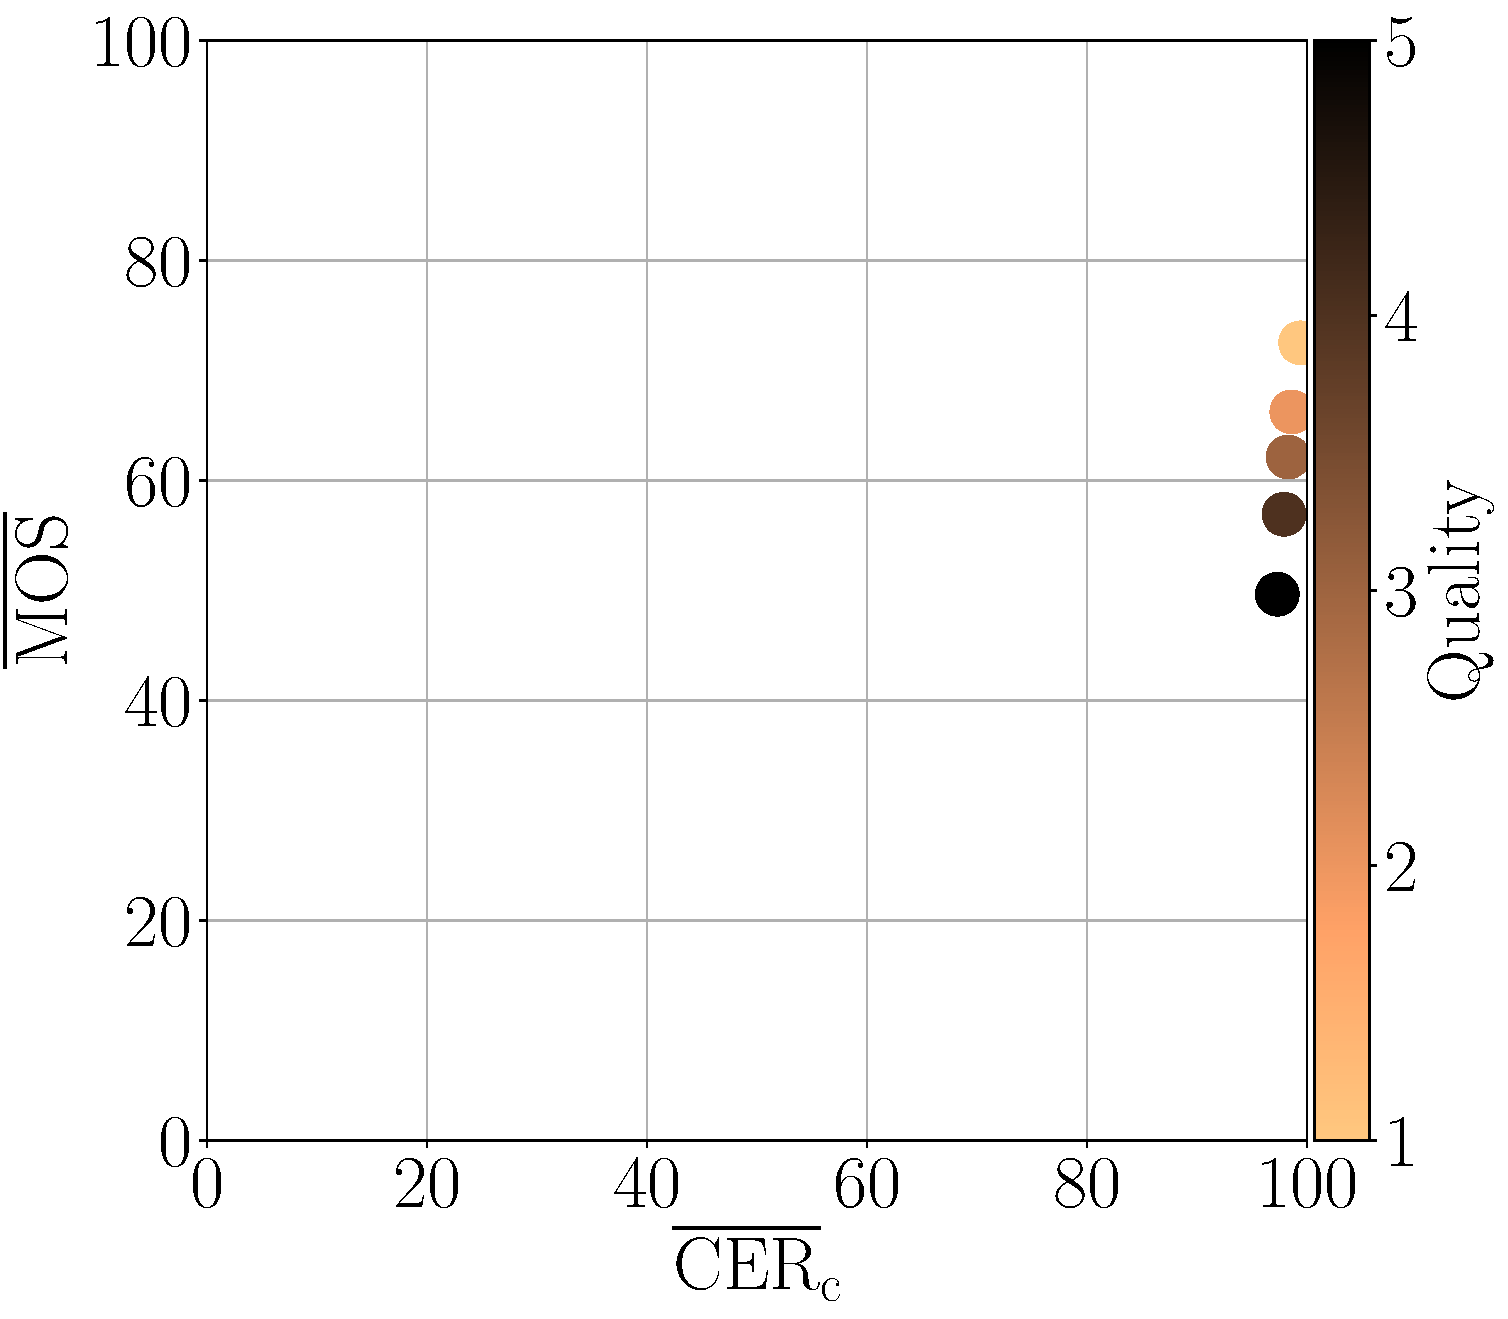
\includegraphics[width=\textwidth]{../../images/analyze/mos_cer_ref_mean_ezocr_CSC.pdf}
        \caption{CSC}
        \label{fig:mos_cer_ref_mean_ezocr_CSC}
    \end{subfigure}
    \hfill
    \begin{subfigure}[b]{0.3\textwidth}
        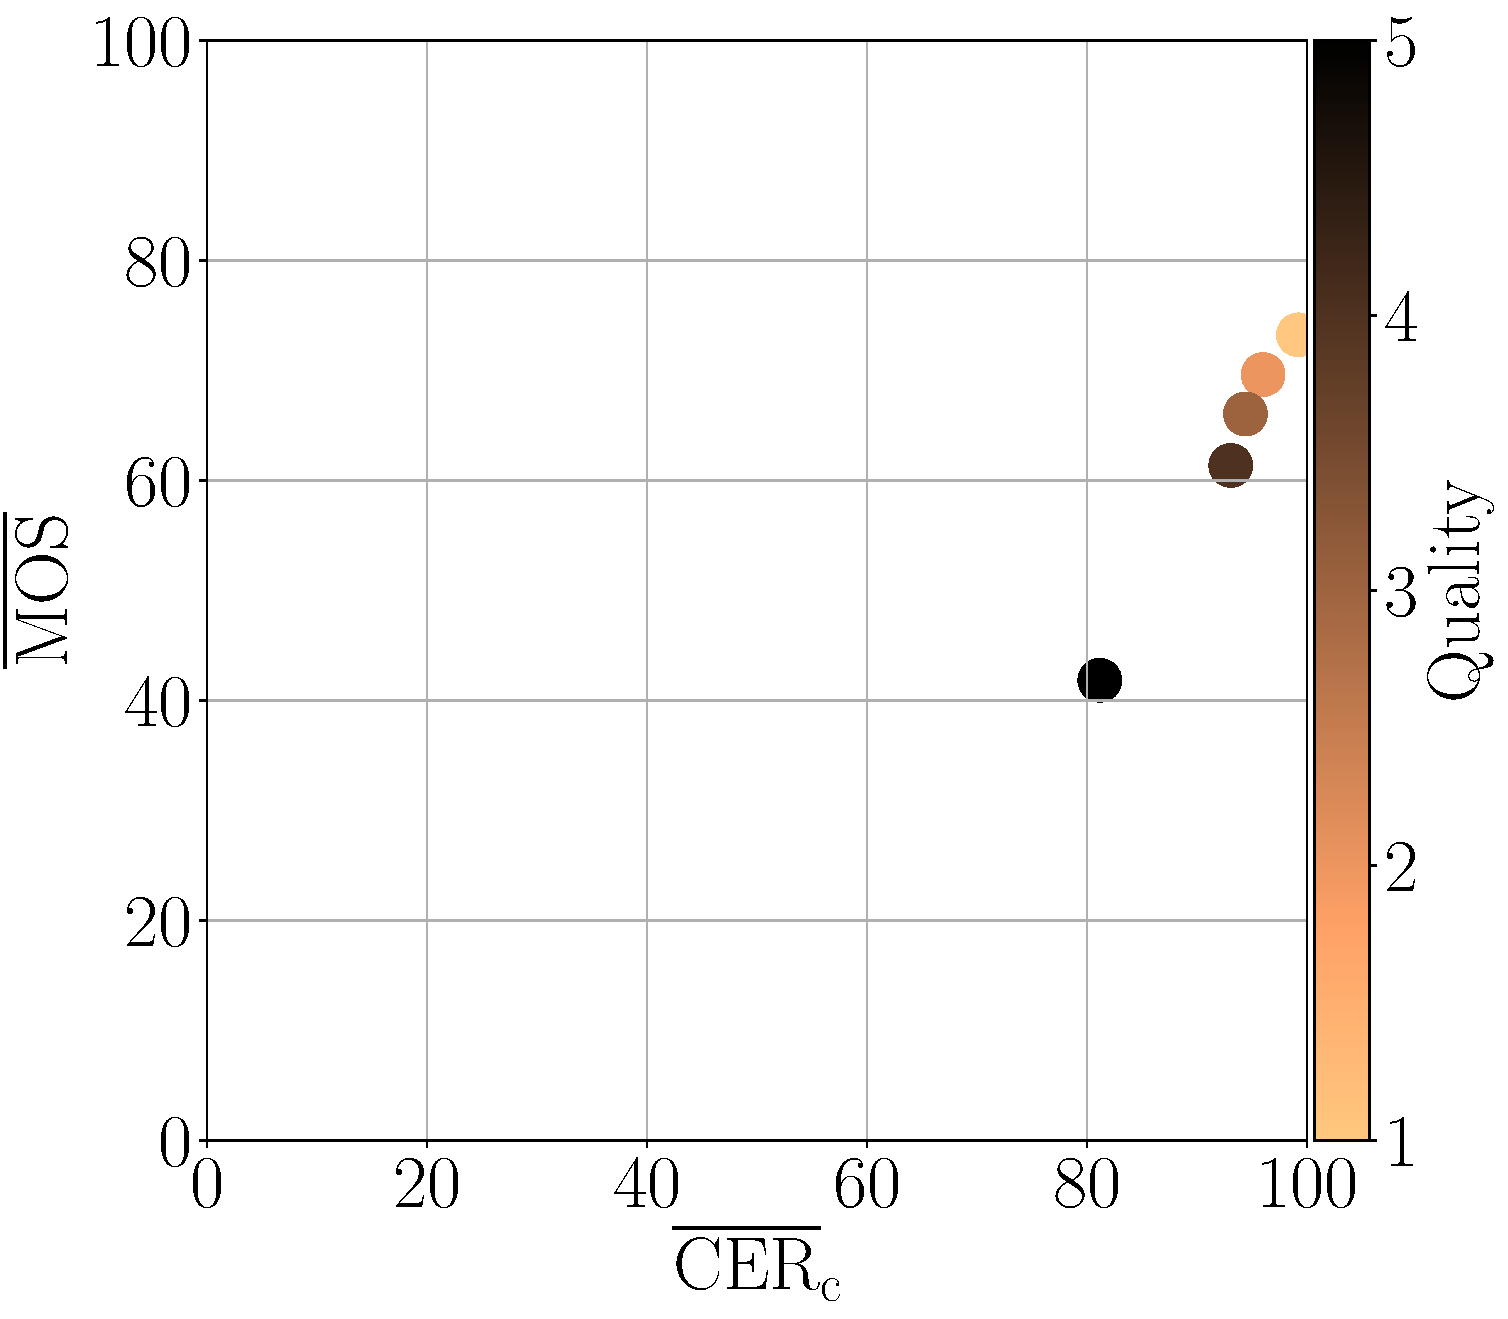
\includegraphics[width=\textwidth]{../../images/analyze/mos_cer_ref_mean_ezocr_HEVC-SCC.pdf}
        \caption{HEVC-SCC}
        \label{fig:mos_cer_ref_mean_ezocr_HEVC-SCC}
    \end{subfigure}
    \hfill
    \begin{subfigure}[b]{0.3\textwidth}
        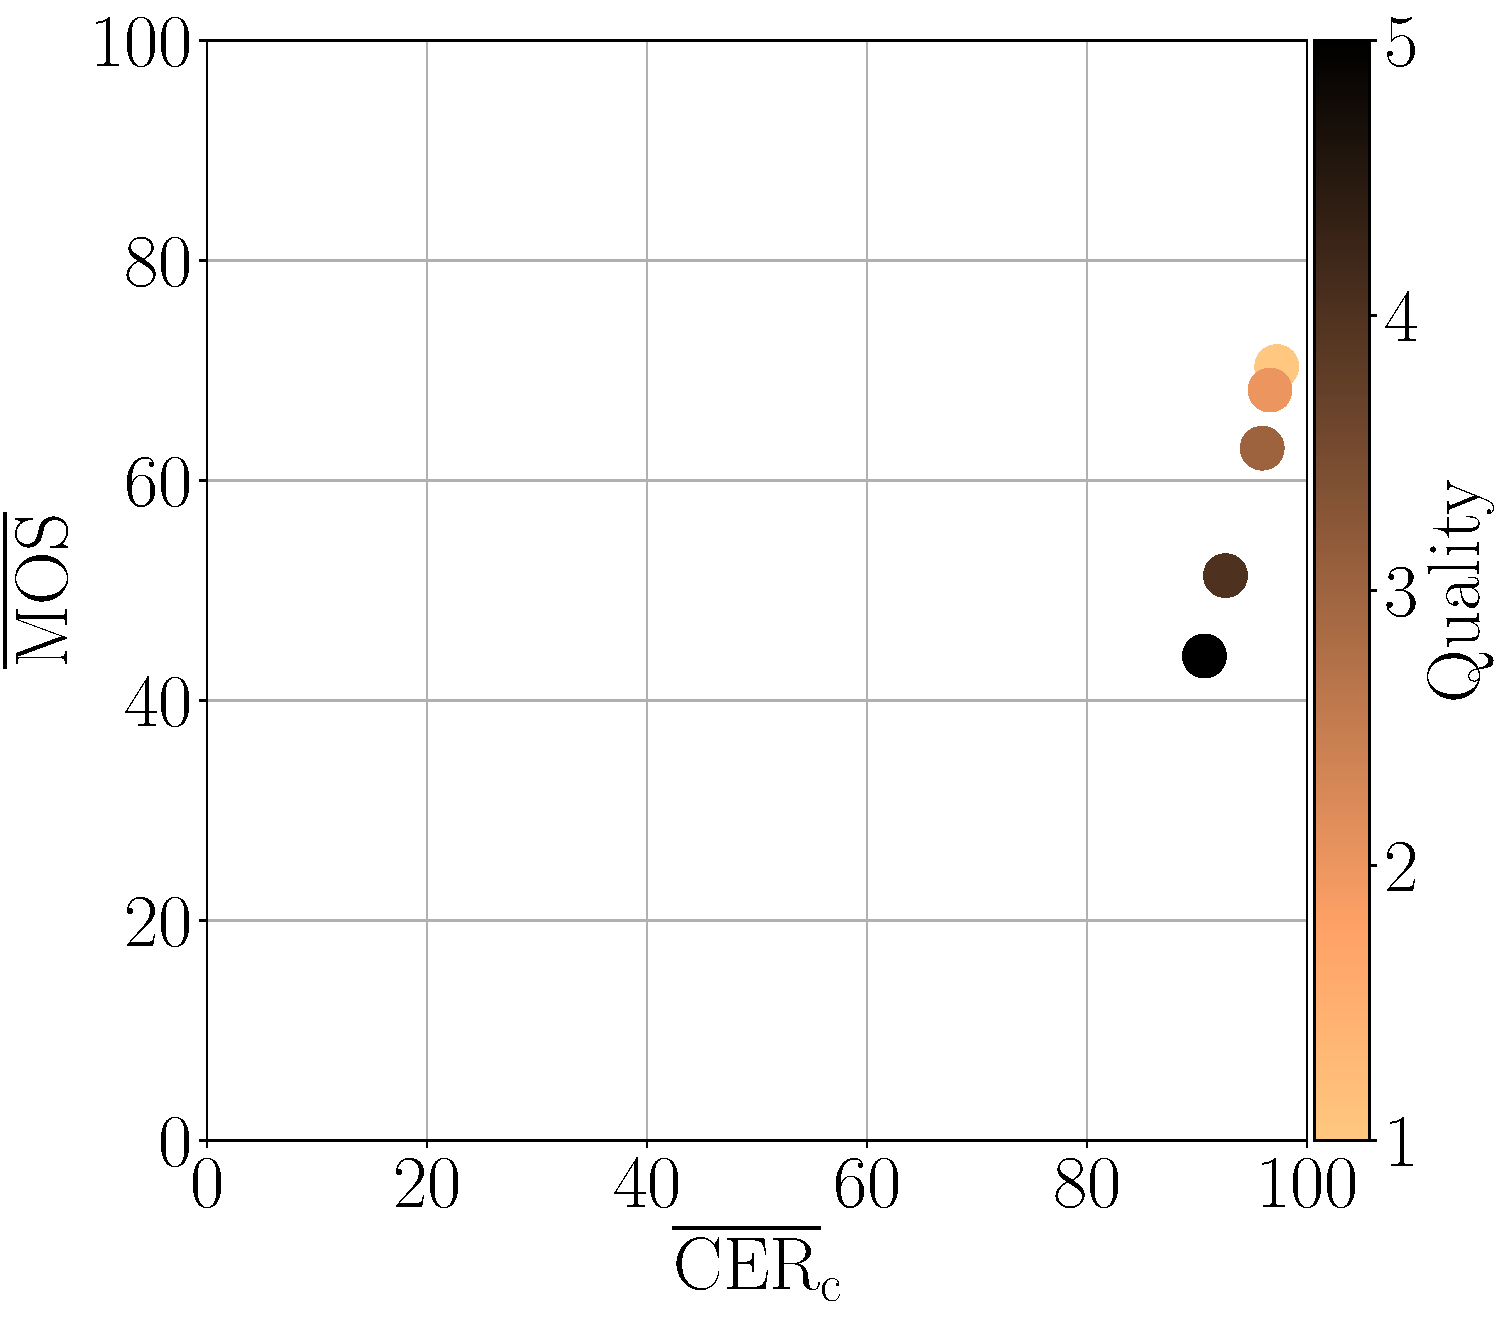
\includegraphics[width=\textwidth]{../../images/analyze/mos_cer_ref_mean_ezocr_CQD.pdf}
        \caption{CQD}
        \label{fig:mos_cer_ref_mean_ezocr_CQD}
    \end{subfigure}
\caption{Mean $\text{CER}_{\text{c}}$ in relation to the reference against mean \gls{mos} for different distortion types with EasyOCR.}
\label{fig:mos_cer_ref_mean_ezocr}
\end{figure}

In \autoref{fig:mos_cer_ref_mean_ezocr} we can see the mean $\text{CER}_{\text{c}}$ in relation to the reference image against the mean \gls{mos} over selected images for all distortions with EasyOCR.
The first general thing to notice is that the performance ceiling for the $\text{CER}_{\text{c}}$ is now up to almost 100.
This is because the $\text{CER}_{\text{c}}$ is calculated in relation to the reference image, which is not necessarily the ground truth.
So it is clear, that the performance on CSC and CC are not impacted much by the distortions, as we saw in the previous section.
The \gls{mos} for CSC varies more than the $\text{CER}_{\text{c}}$, but not as much as for other distortion types.
This suggests at least a slight correlation between the \gls{mos} and the $\text{CER}_{\text{c}}$.
For CC neither metric shows a clear trend.
It is not clear why the \gls{mos} for CC is not strictly decreasing with the quality level.
All other distortions show this trend.
Contrast levels do not clearly reach from good to bad, it might be that humans found specific contrast levels more appealing than others.

% mos vs cer mean in relation to reference for Tesseract
\begin{figure}[h]
\centering
    \begin{subfigure}[b]{0.3\textwidth}
        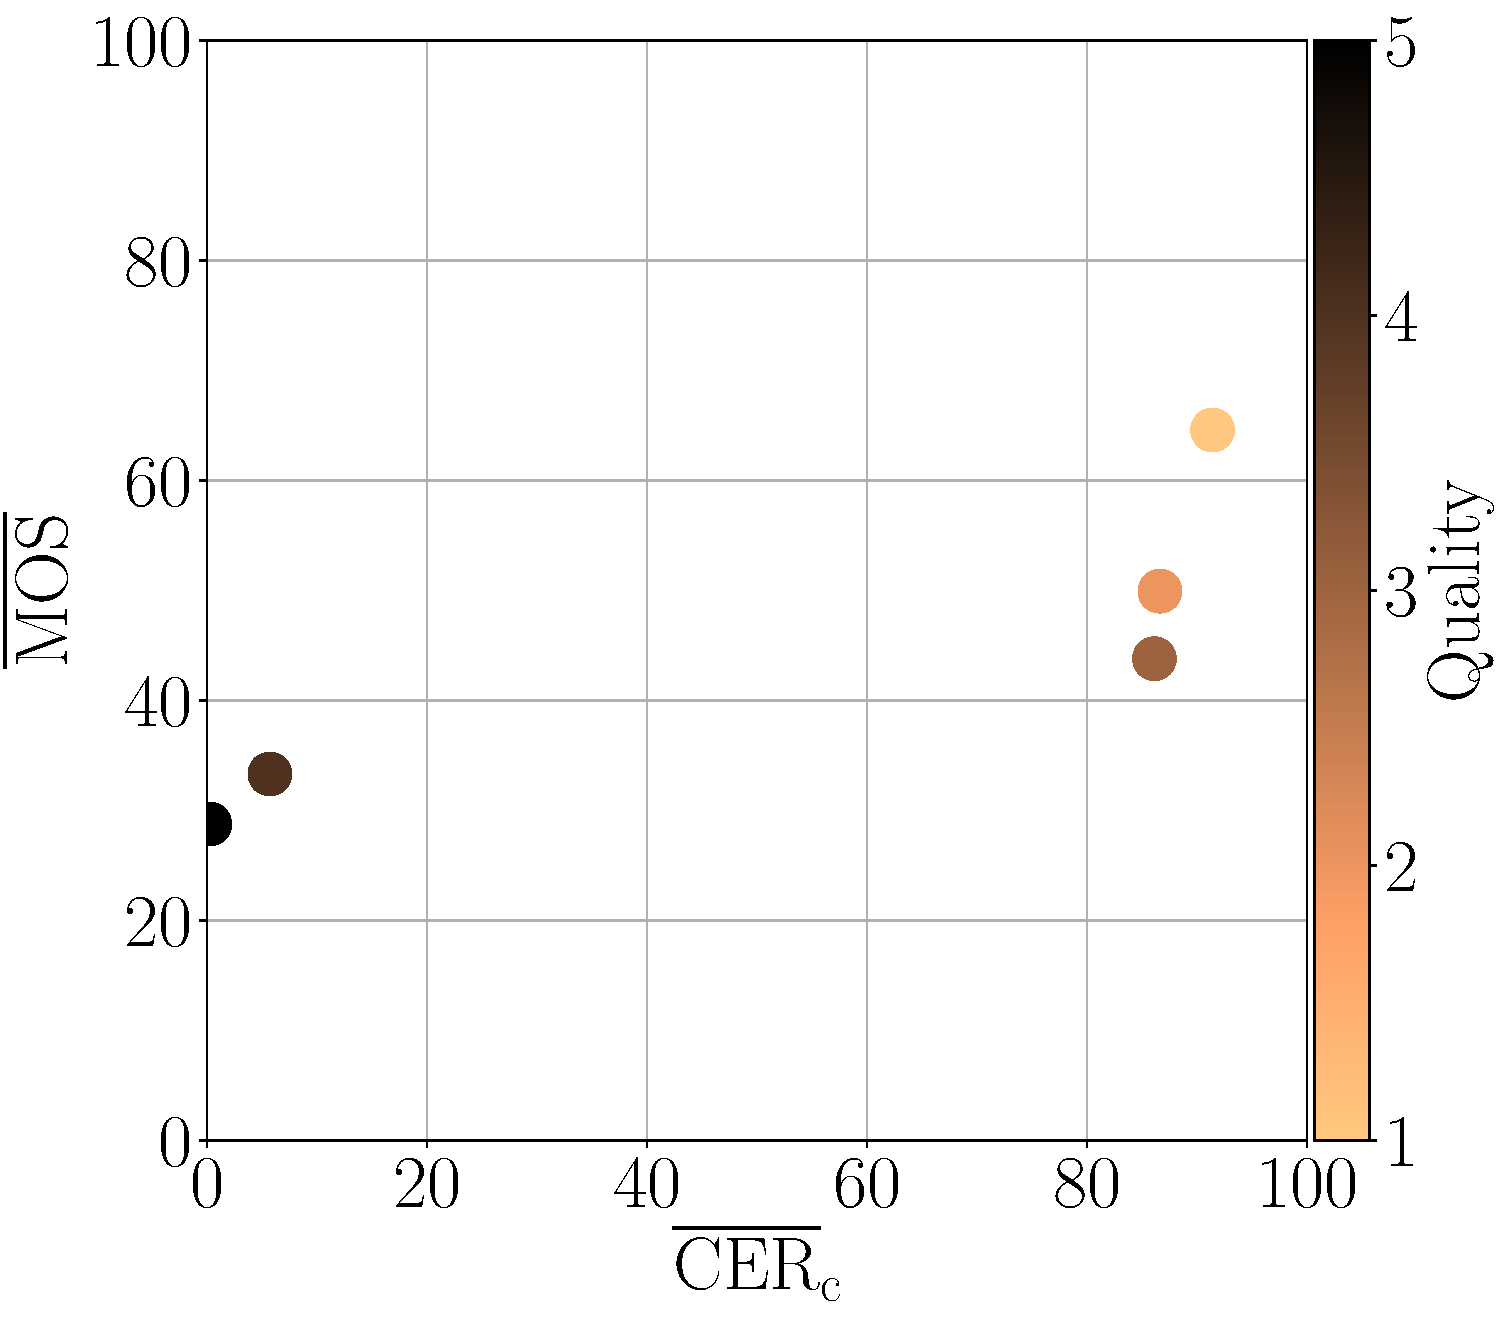
\includegraphics[width=\textwidth]{../../images/analyze/mos_cer_ref_mean_tess_GN.pdf}
        \caption{GN}
        \label{fig:mos_cer_ref_mean_tess_GN}
    \end{subfigure}
    \hfill
    \begin{subfigure}[b]{0.3\textwidth}
        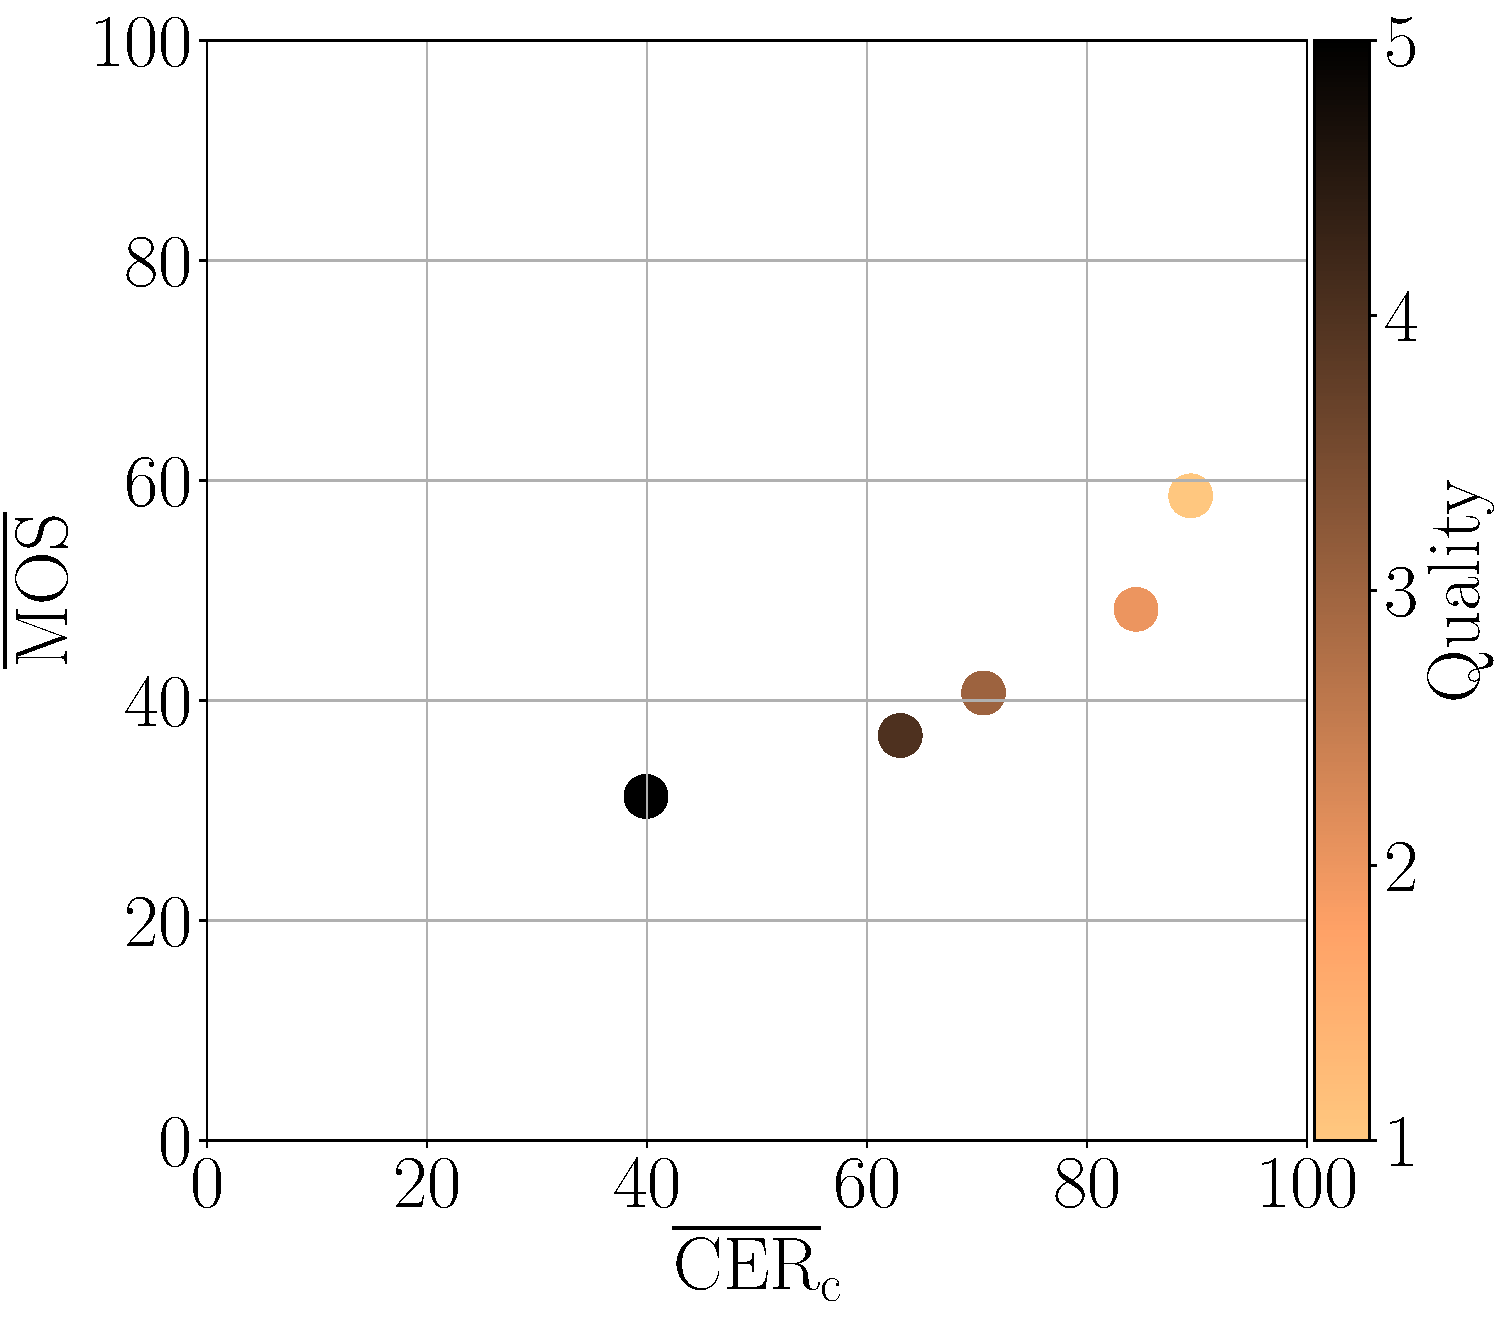
\includegraphics[width=\textwidth]{../../images/analyze/mos_cer_ref_mean_tess_GB.pdf}
        \caption{GB}
        \label{fig:mos_cer_ref_mean_tess_GB}
    \end{subfigure}
    \hfill
    \begin{subfigure}[b]{0.3\textwidth}
        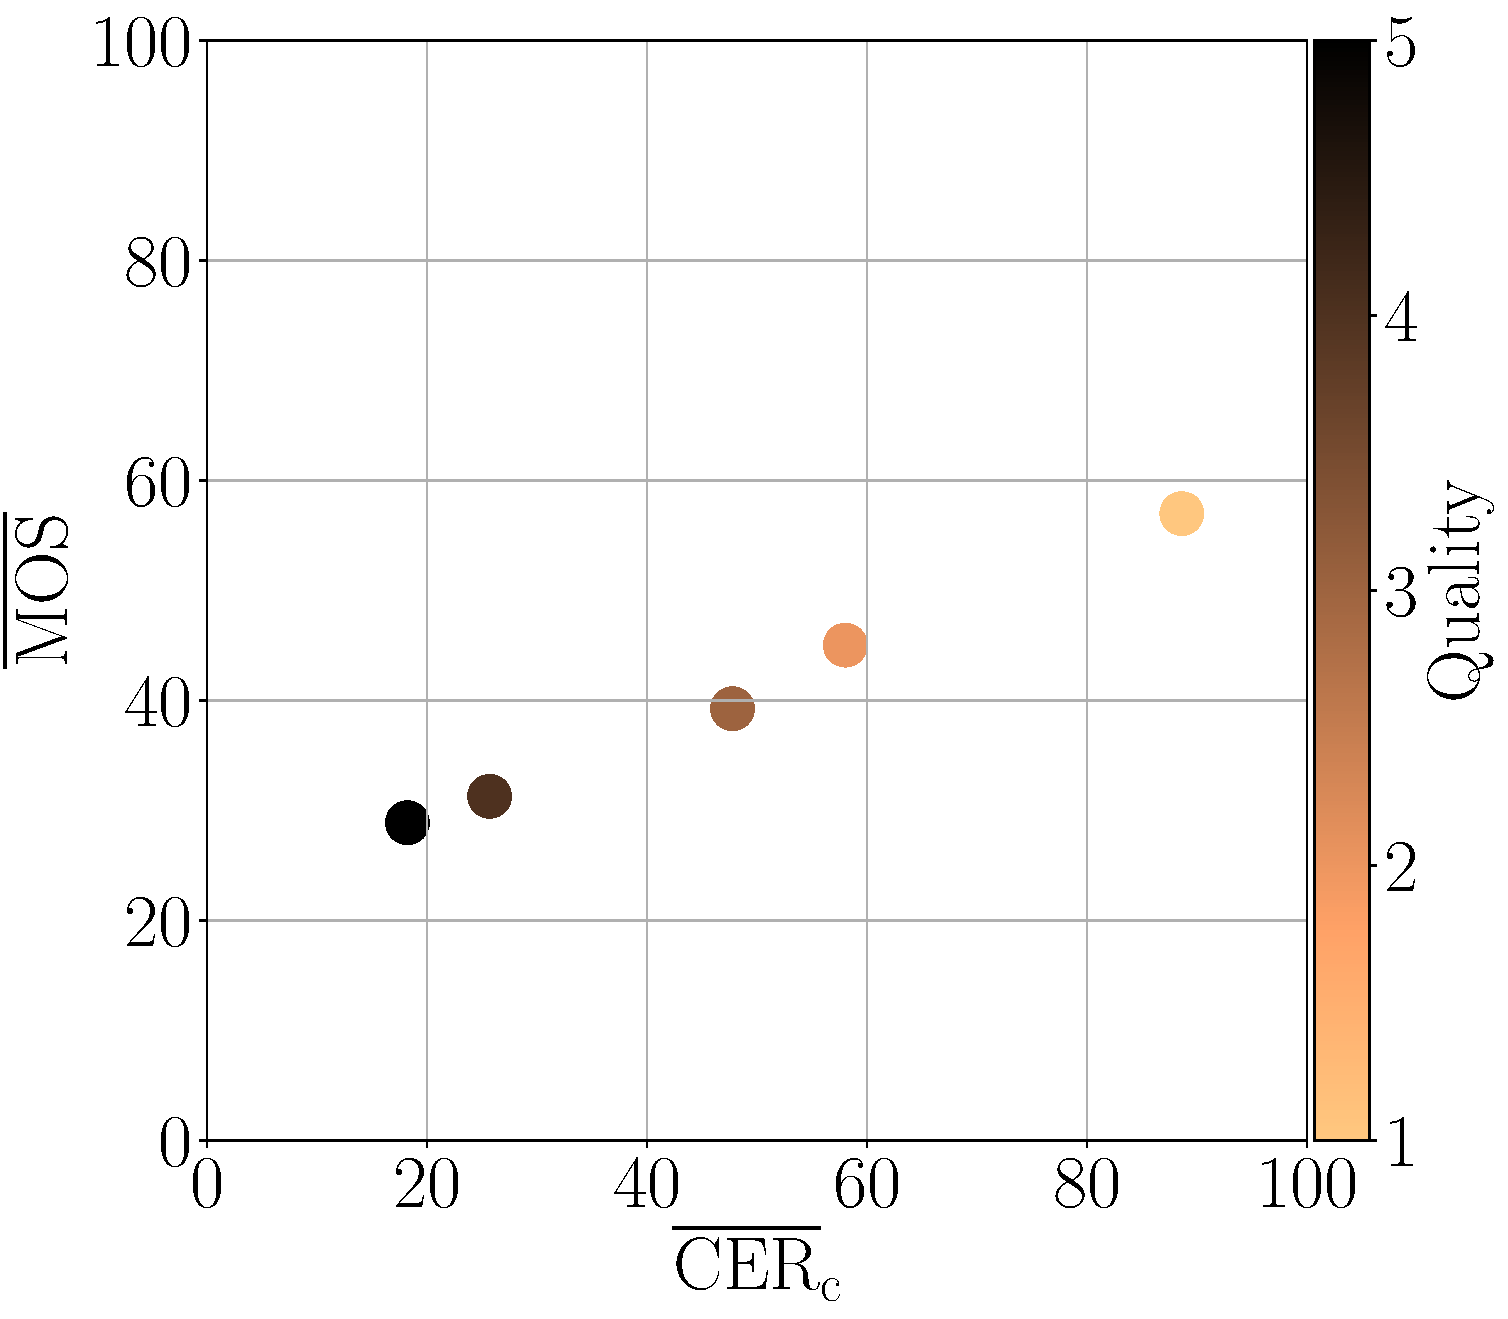
\includegraphics[width=\textwidth]{../../images/analyze/mos_cer_ref_mean_tess_MB.pdf}
        \caption{MB}
        \label{fig:mos_cer_ref_mean_tess_MB}
    \end{subfigure}
    \newline
    \begin{subfigure}[b]{0.3\textwidth}
        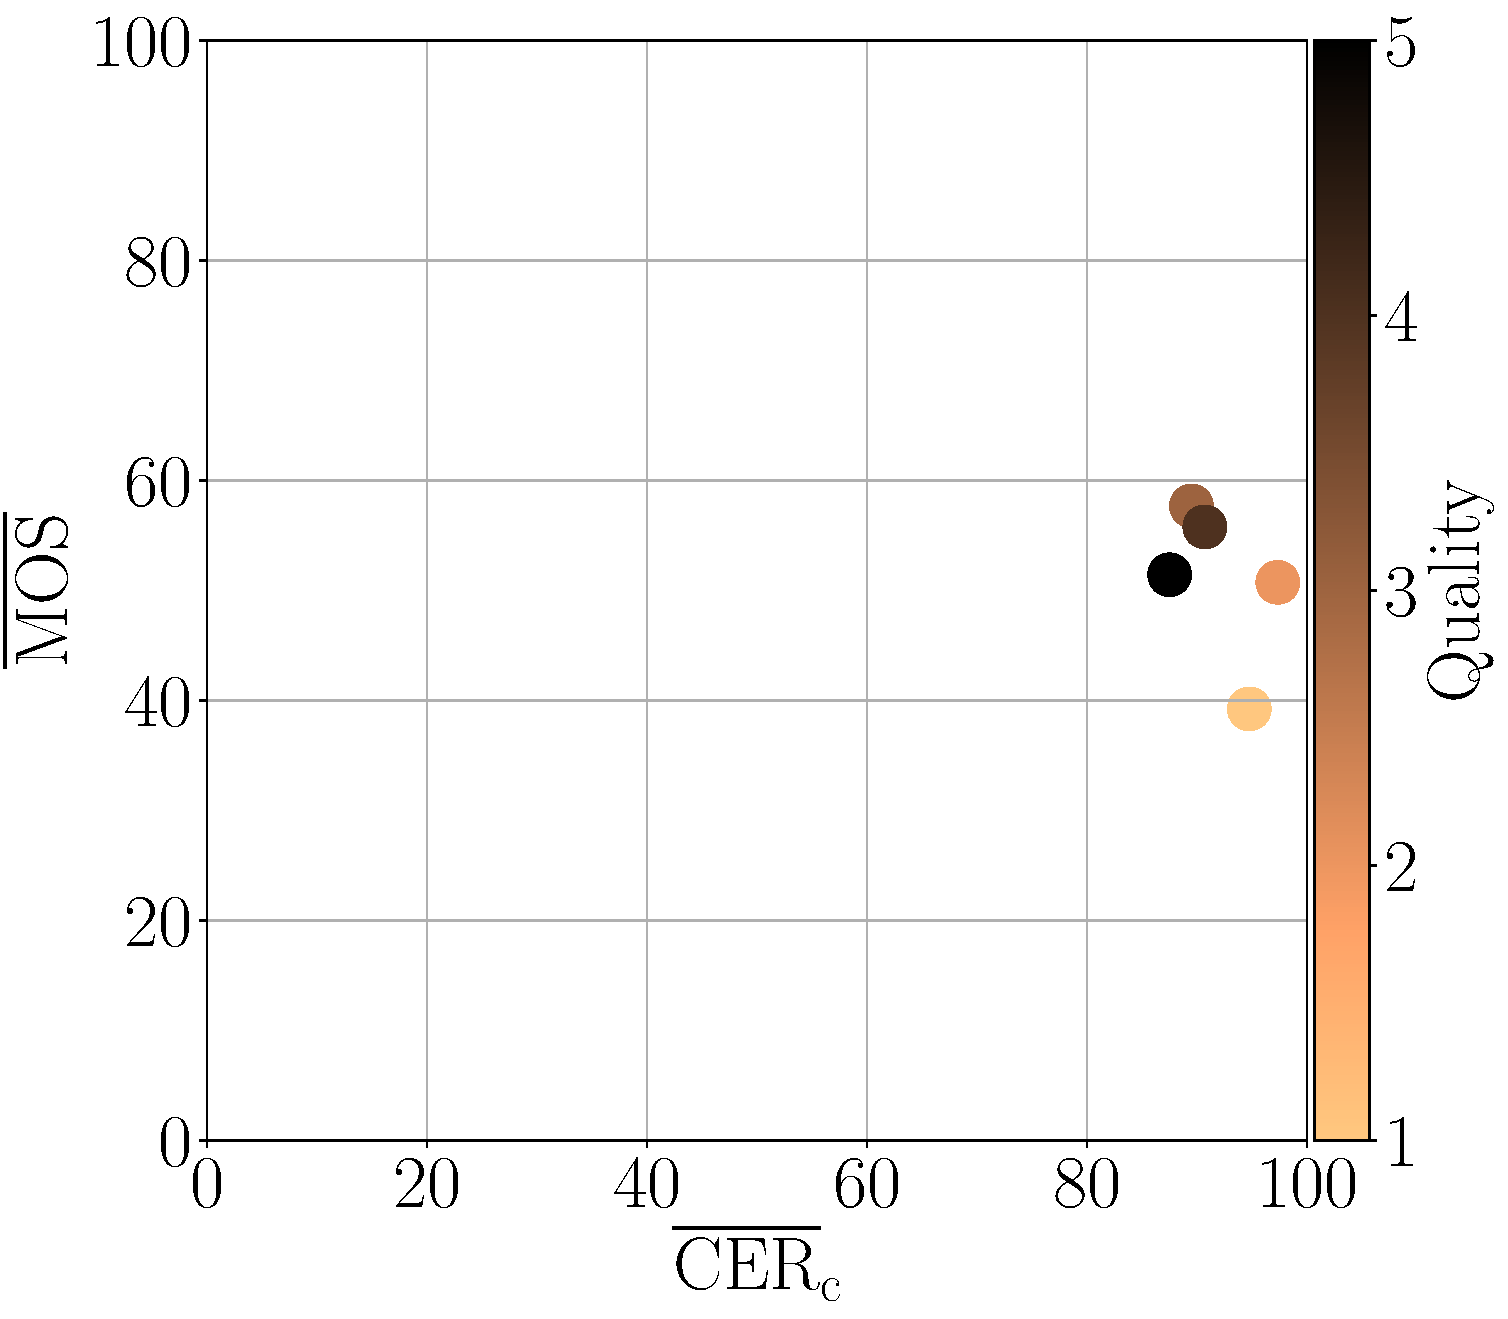
\includegraphics[width=\textwidth]{../../images/analyze/mos_cer_ref_mean_tess_CC.pdf}
        \caption{CC}
        \label{fig:mos_cer_ref_mean_tess_CC}
    \end{subfigure}
    \hfill
    \begin{subfigure}[b]{0.3\textwidth}
        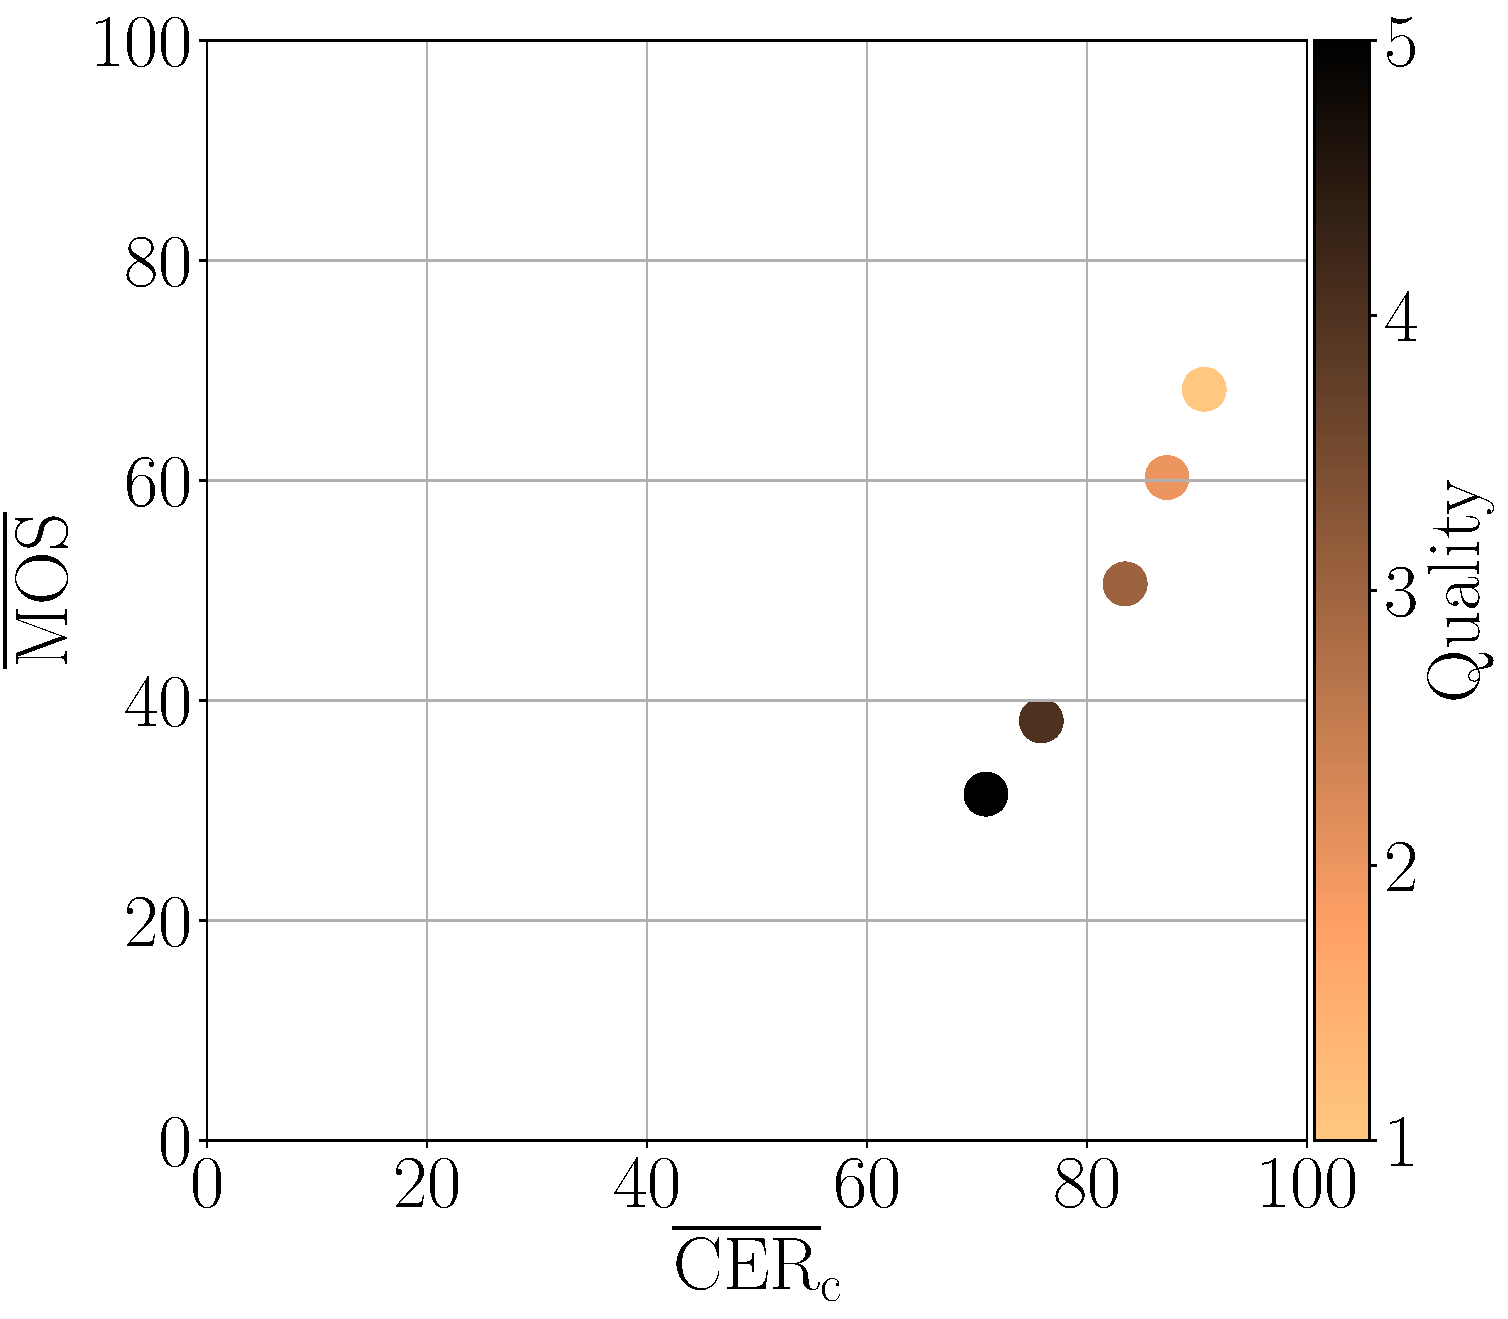
\includegraphics[width=\textwidth]{../../images/analyze/mos_cer_ref_mean_tess_JPEG.pdf}
        \caption{JPEG}
        \label{fig:mos_cer_ref_mean_tess_JPEG}
    \end{subfigure}
    \hfill
    \begin{subfigure}[b]{0.3\textwidth}
        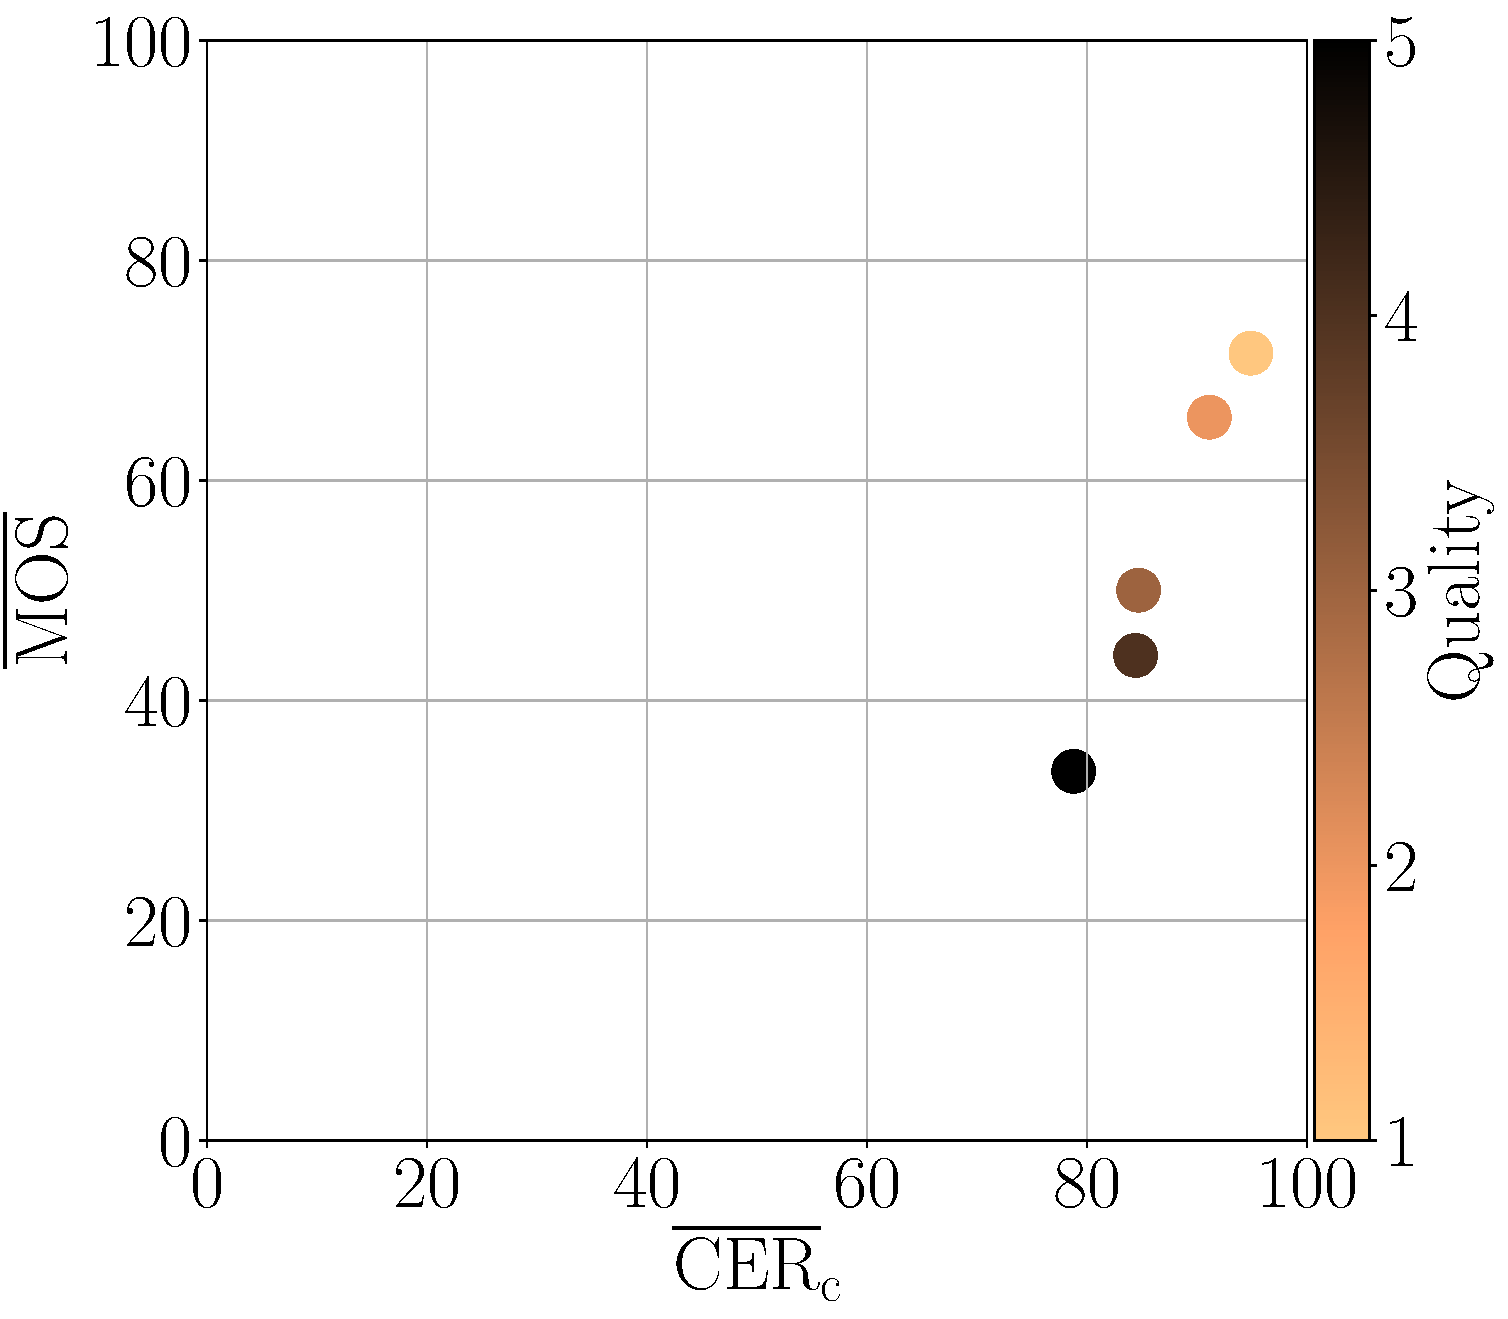
\includegraphics[width=\textwidth]{../../images/analyze/mos_cer_ref_mean_tess_JPEG2000.pdf}
        \caption{JPEG2000}
        \label{fig:mos_cer_ref_mean_tess_JPEG2000}
    \end{subfigure}
    \newline
    \begin{subfigure}[b]{0.3\textwidth}
        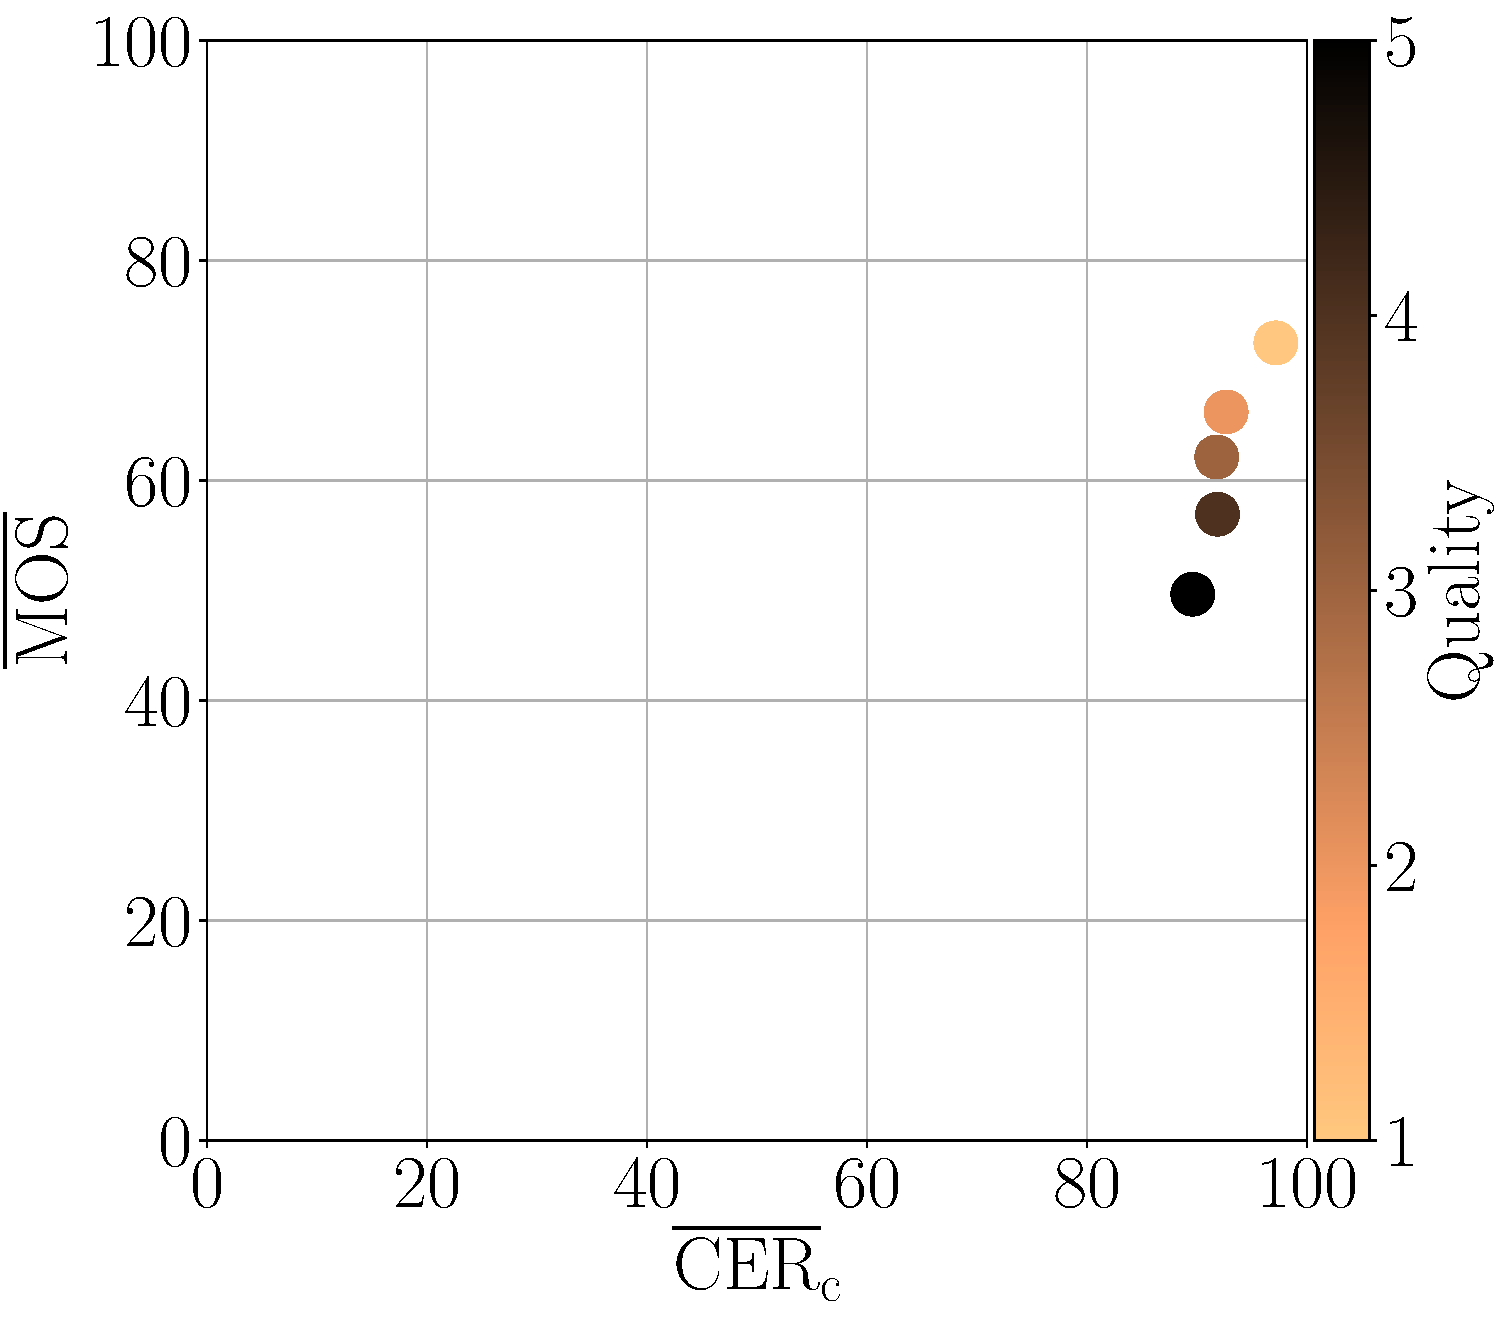
\includegraphics[width=\textwidth]{../../images/analyze/mos_cer_ref_mean_tess_CSC.pdf}
        \caption{CSC}
        \label{fig:mos_cer_ref_mean_tess_CSC}
    \end{subfigure}
    \hfill
    \begin{subfigure}[b]{0.3\textwidth}
        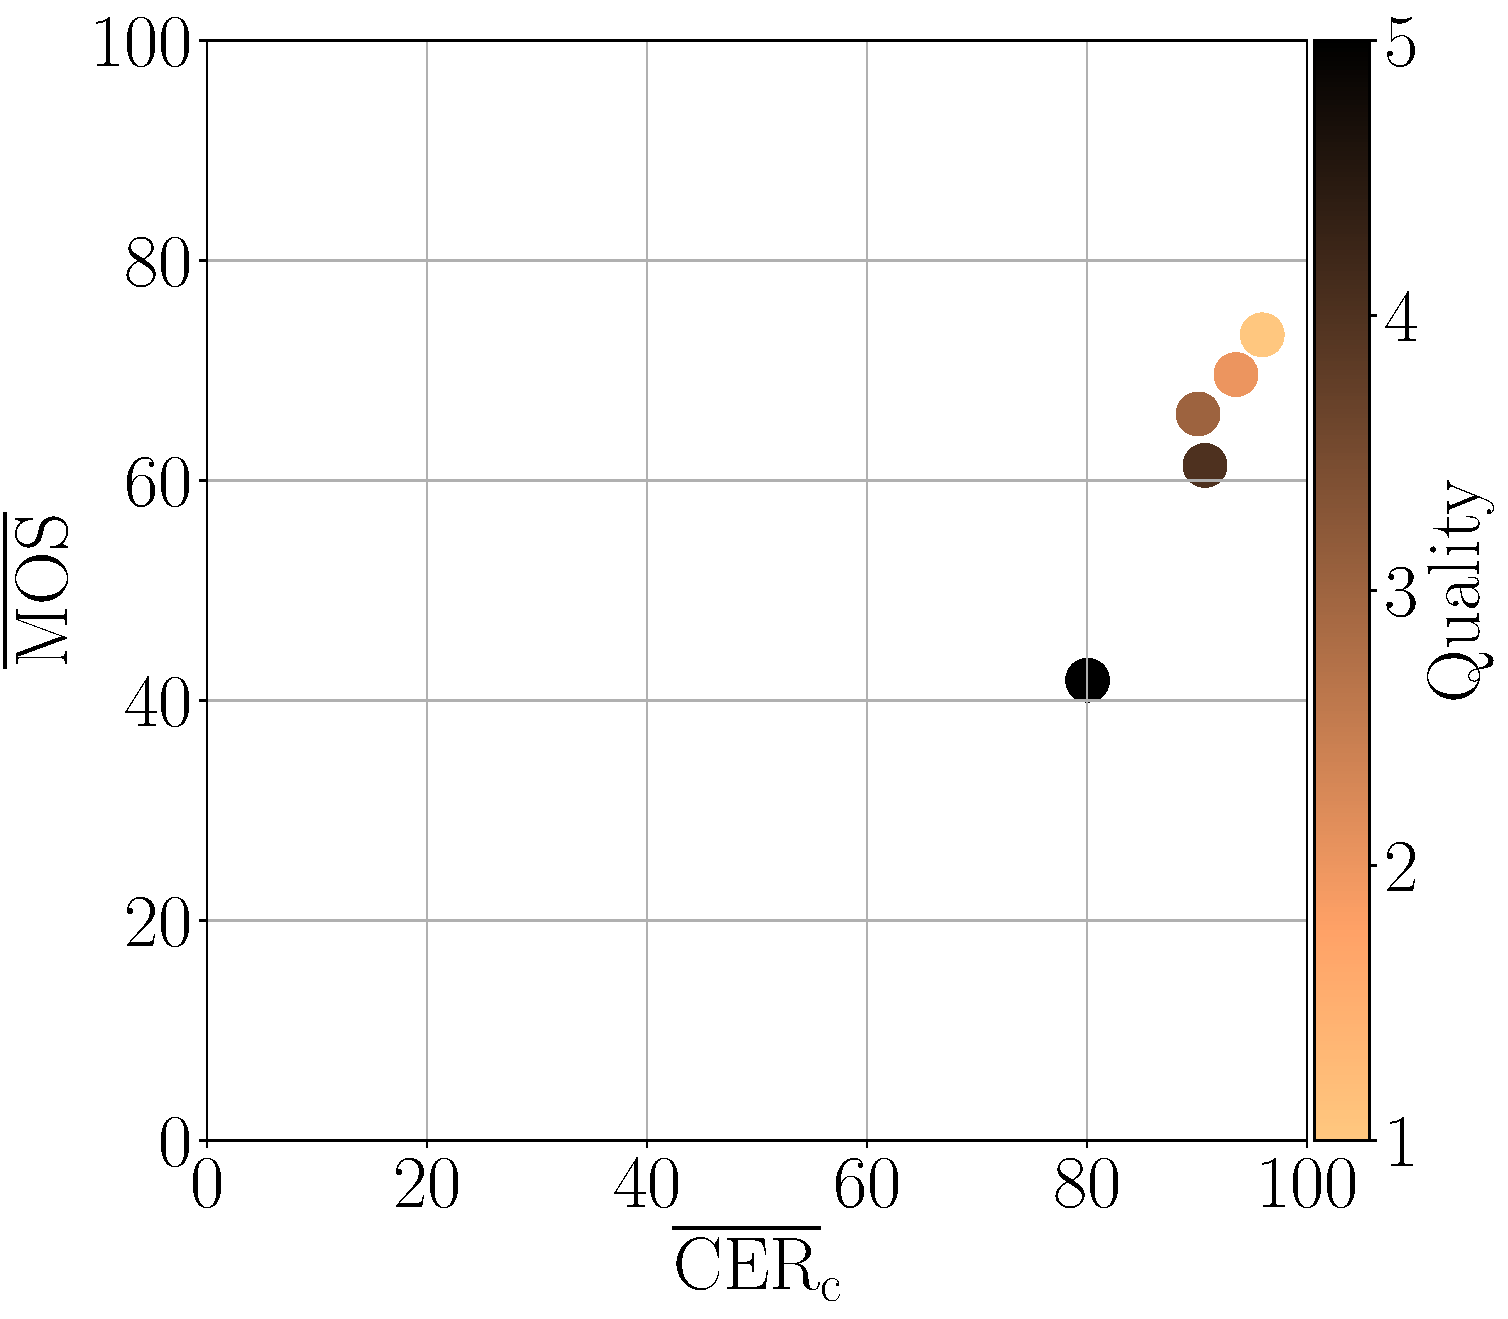
\includegraphics[width=\textwidth]{../../images/analyze/mos_cer_ref_mean_tess_HEVC-SCC.pdf}
        \caption{HEVC-SCC}
        \label{fig:mos_cer_ref_mean_tess_HEVC-SCC}
    \end{subfigure}
    \hfill
    \begin{subfigure}[b]{0.3\textwidth}
        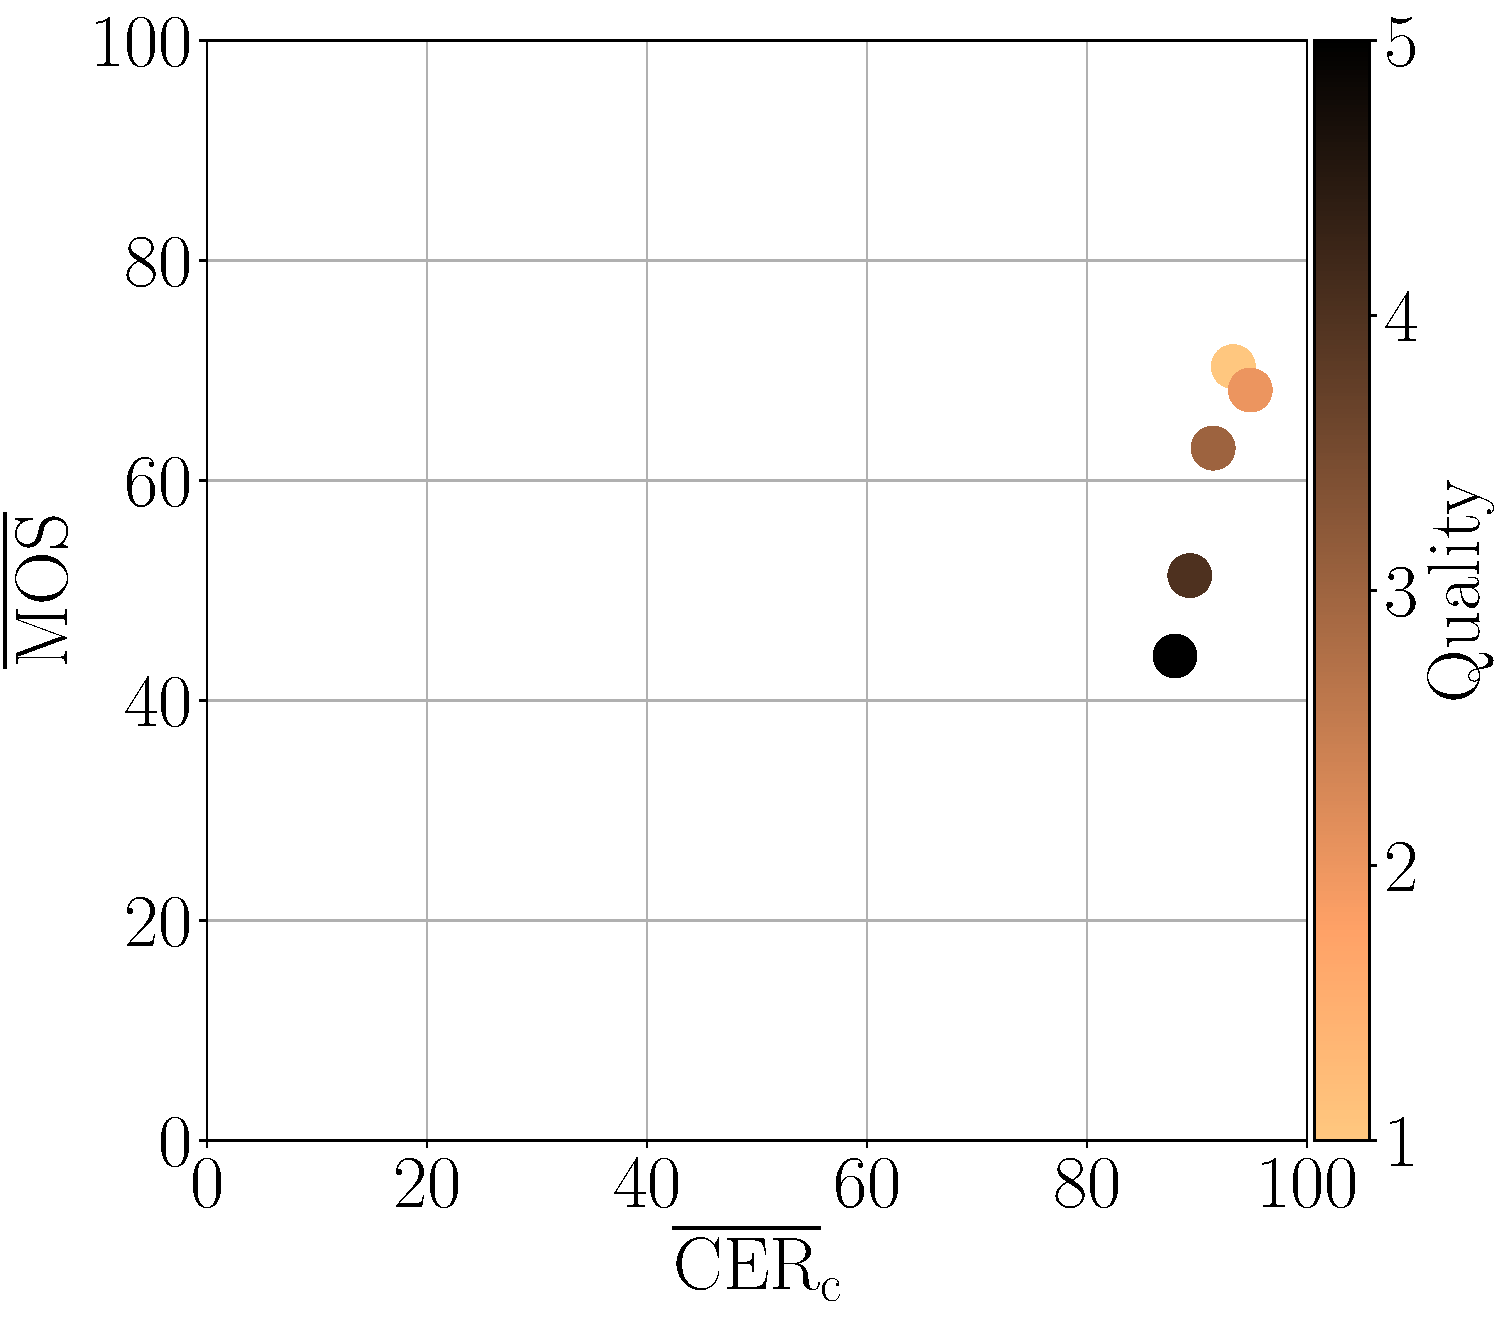
\includegraphics[width=\textwidth]{../../images/analyze/mos_cer_ref_mean_tess_CQD.pdf}
        \caption{CQD}
        \label{fig:mos_cer_ref_mean_tess_CQD}
    \end{subfigure}
    \caption{Mean $\text{CER}_{\text{c}}$ in relation to the reference against mean \gls{mos} for different distortion types with Tesseract \gls{ocr}.}
\label{fig:mos_cer_ref_mean_tess}
\end{figure}

In \autoref{fig:mos_cer_ref_mean_tess} we can see the mean $\text{CER}_{\text{c}}$ against the mean \gls{mos} over selected images for all distortions with Tesseract \gls{ocr}.


% mos vs cer (fitted) mean in relation to reference for ezocr
\begin{figure}[h]
\centering
    \begin{subfigure}[b]{0.3\textwidth}
        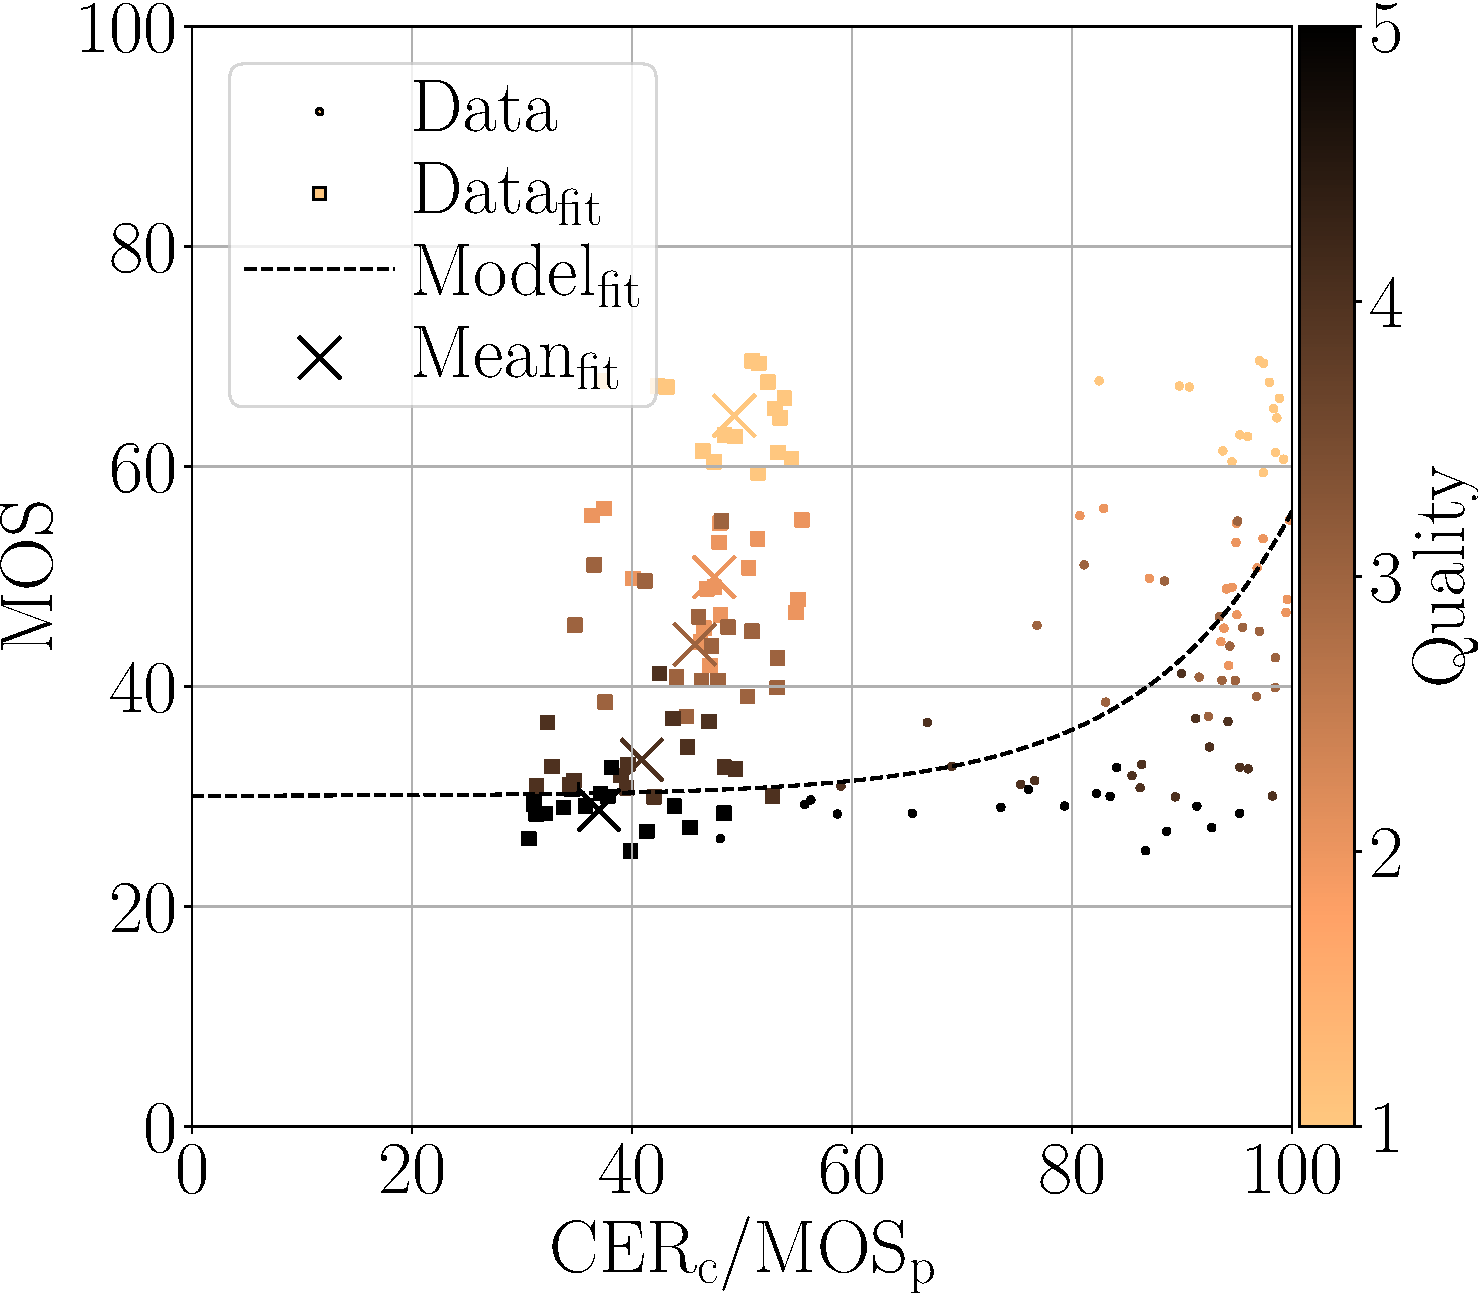
\includegraphics[width=\textwidth]{../../images/analyze/mos_cer_ref_fitted_mean_ezocr_GN.pdf}
        \caption{GN}
        \label{fig:mos_cer_ref_fitted_mean_ezocr_GN}
    \end{subfigure}
    \hfill
    \begin{subfigure}[b]{0.3\textwidth}
        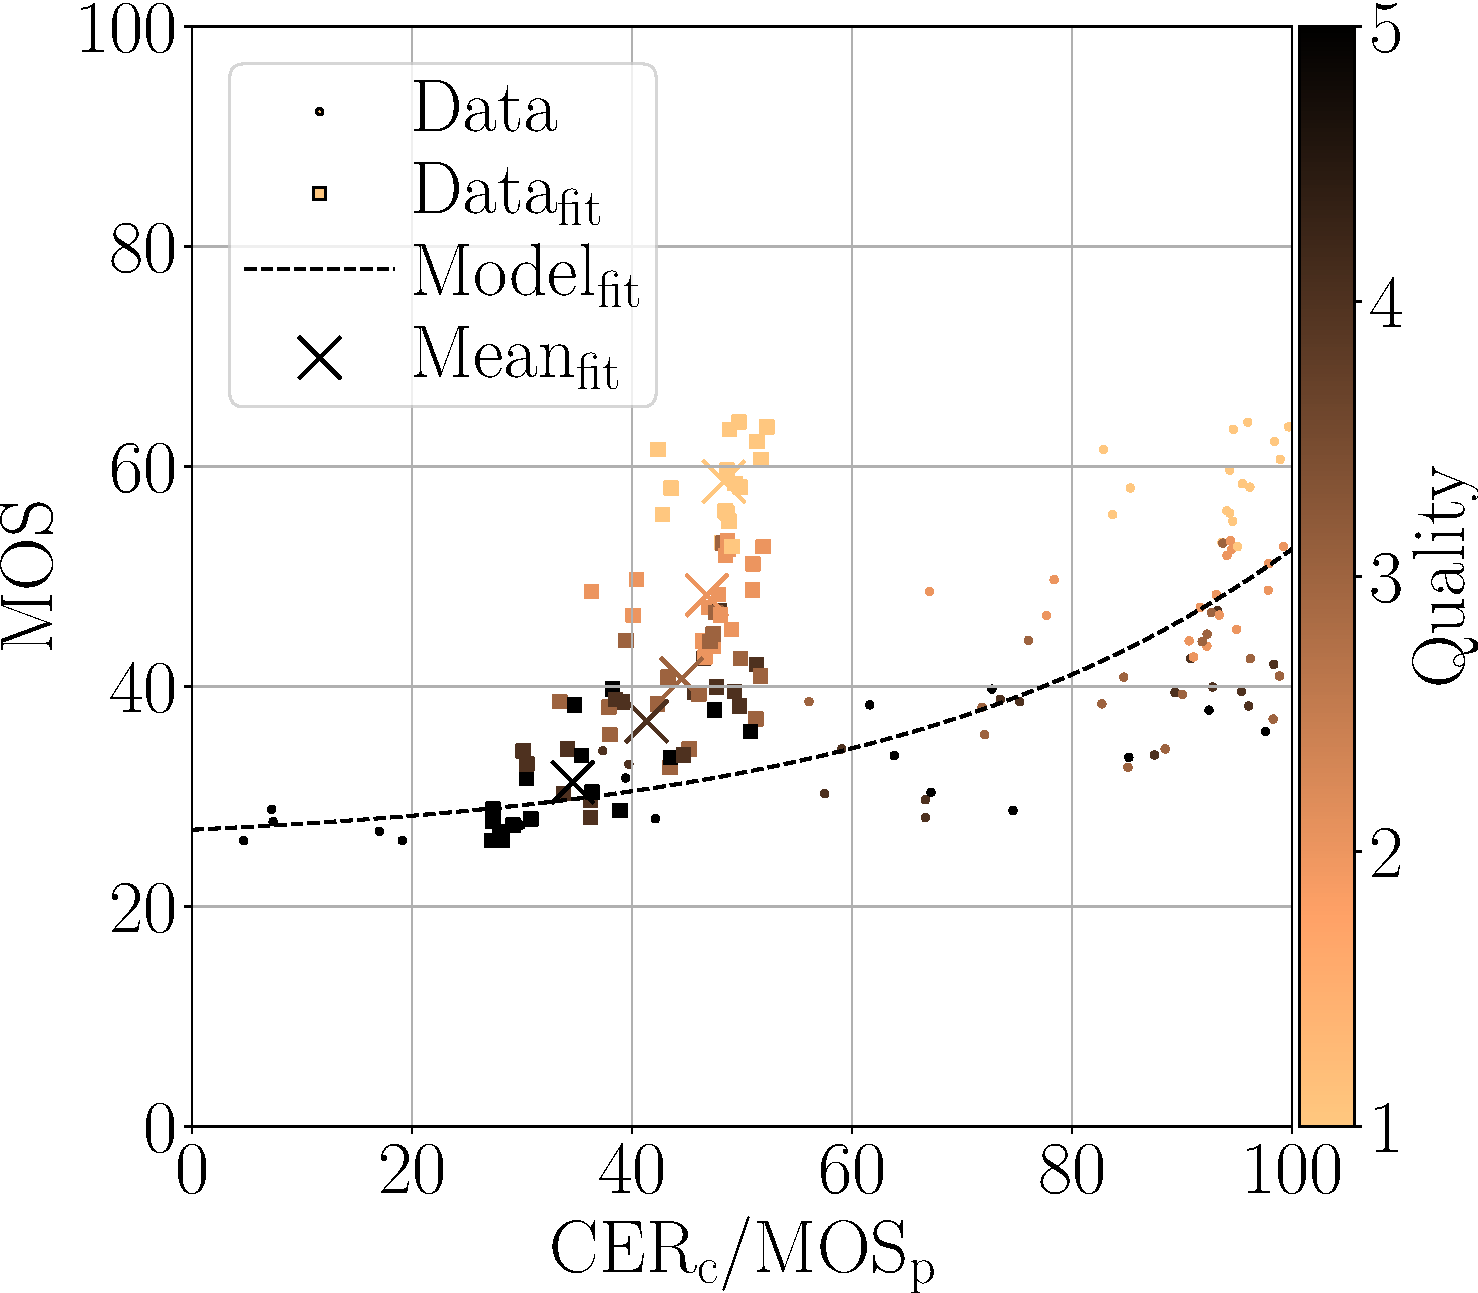
\includegraphics[width=\textwidth]{../../images/analyze/mos_cer_ref_fitted_mean_ezocr_GB.pdf}
        \caption{GB}
        \label{fig:mos_cer_ref_fitted_mean_ezocr_GB}
    \end{subfigure}
    \hfill
    \begin{subfigure}[b]{0.3\textwidth}
        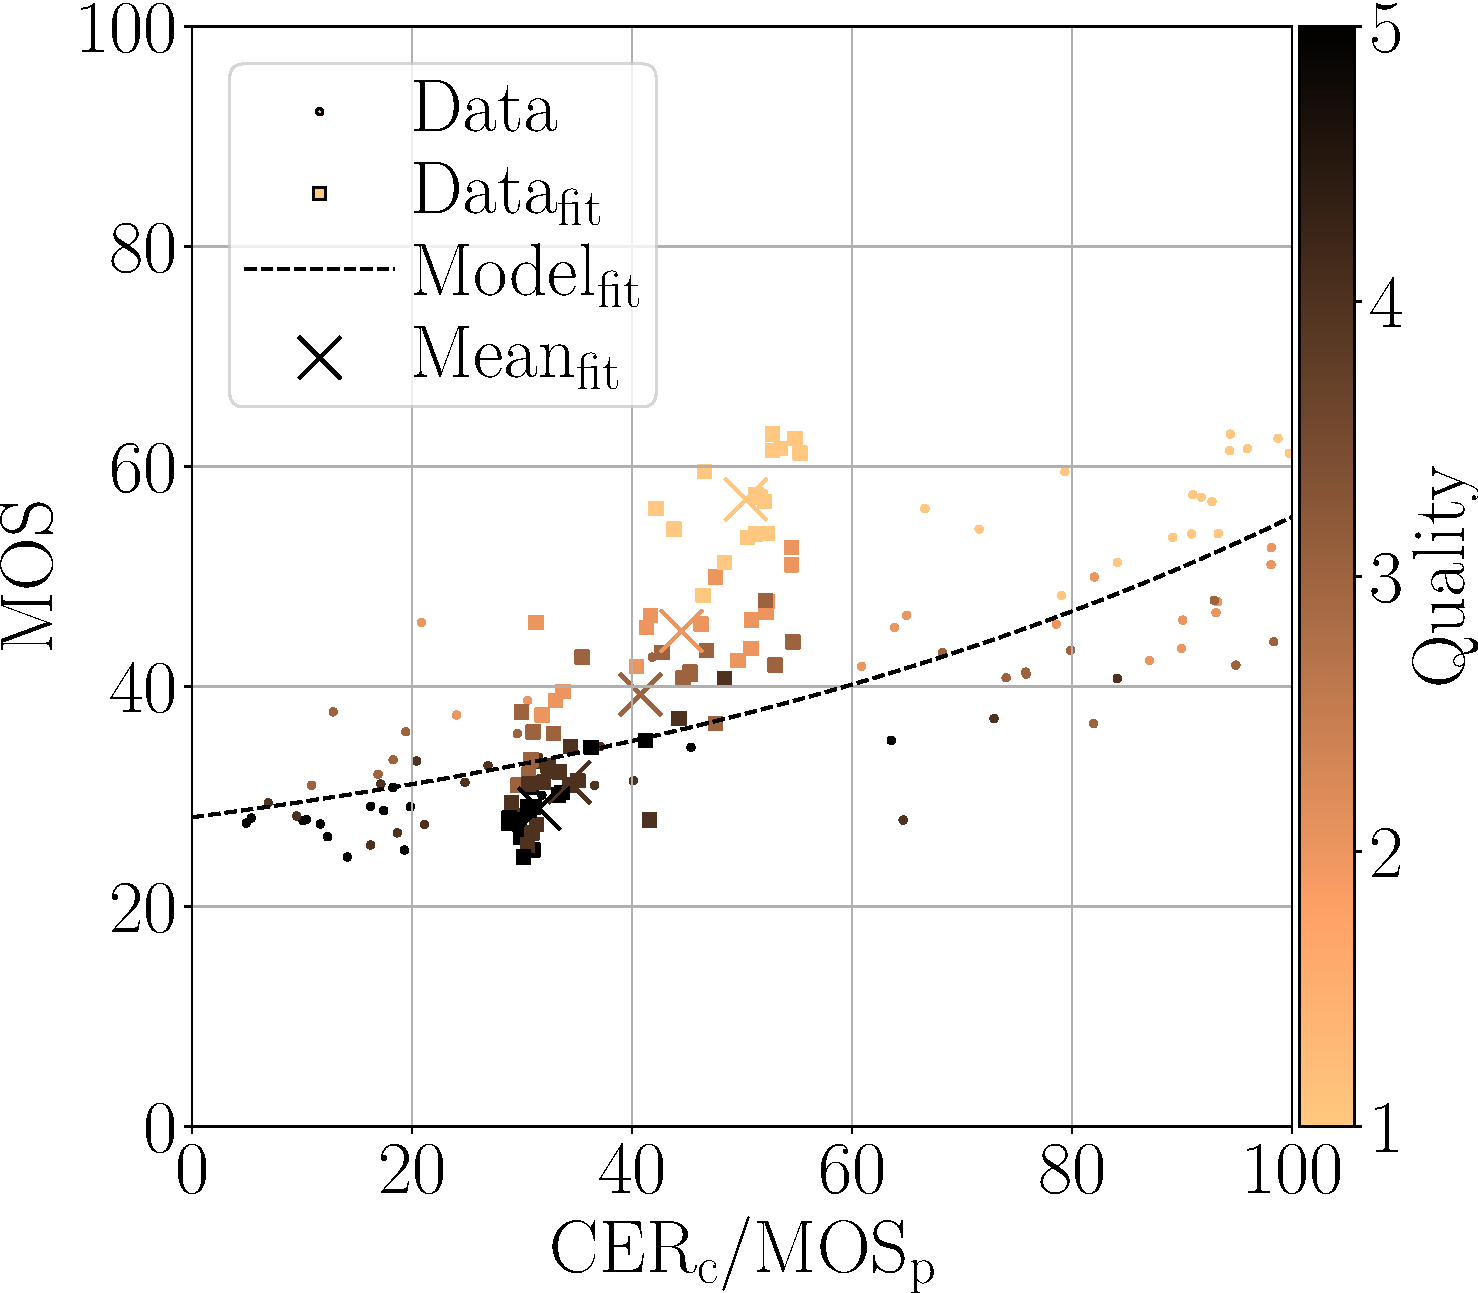
\includegraphics[width=\textwidth]{../../images/analyze/mos_cer_ref_fitted_mean_ezocr_MB.pdf}
        \caption{MB}
        \label{fig:mos_cer_ref_fitted_mean_ezocr_MB}
    \end{subfigure}
    \newline
    \begin{subfigure}[b]{0.3\textwidth}
        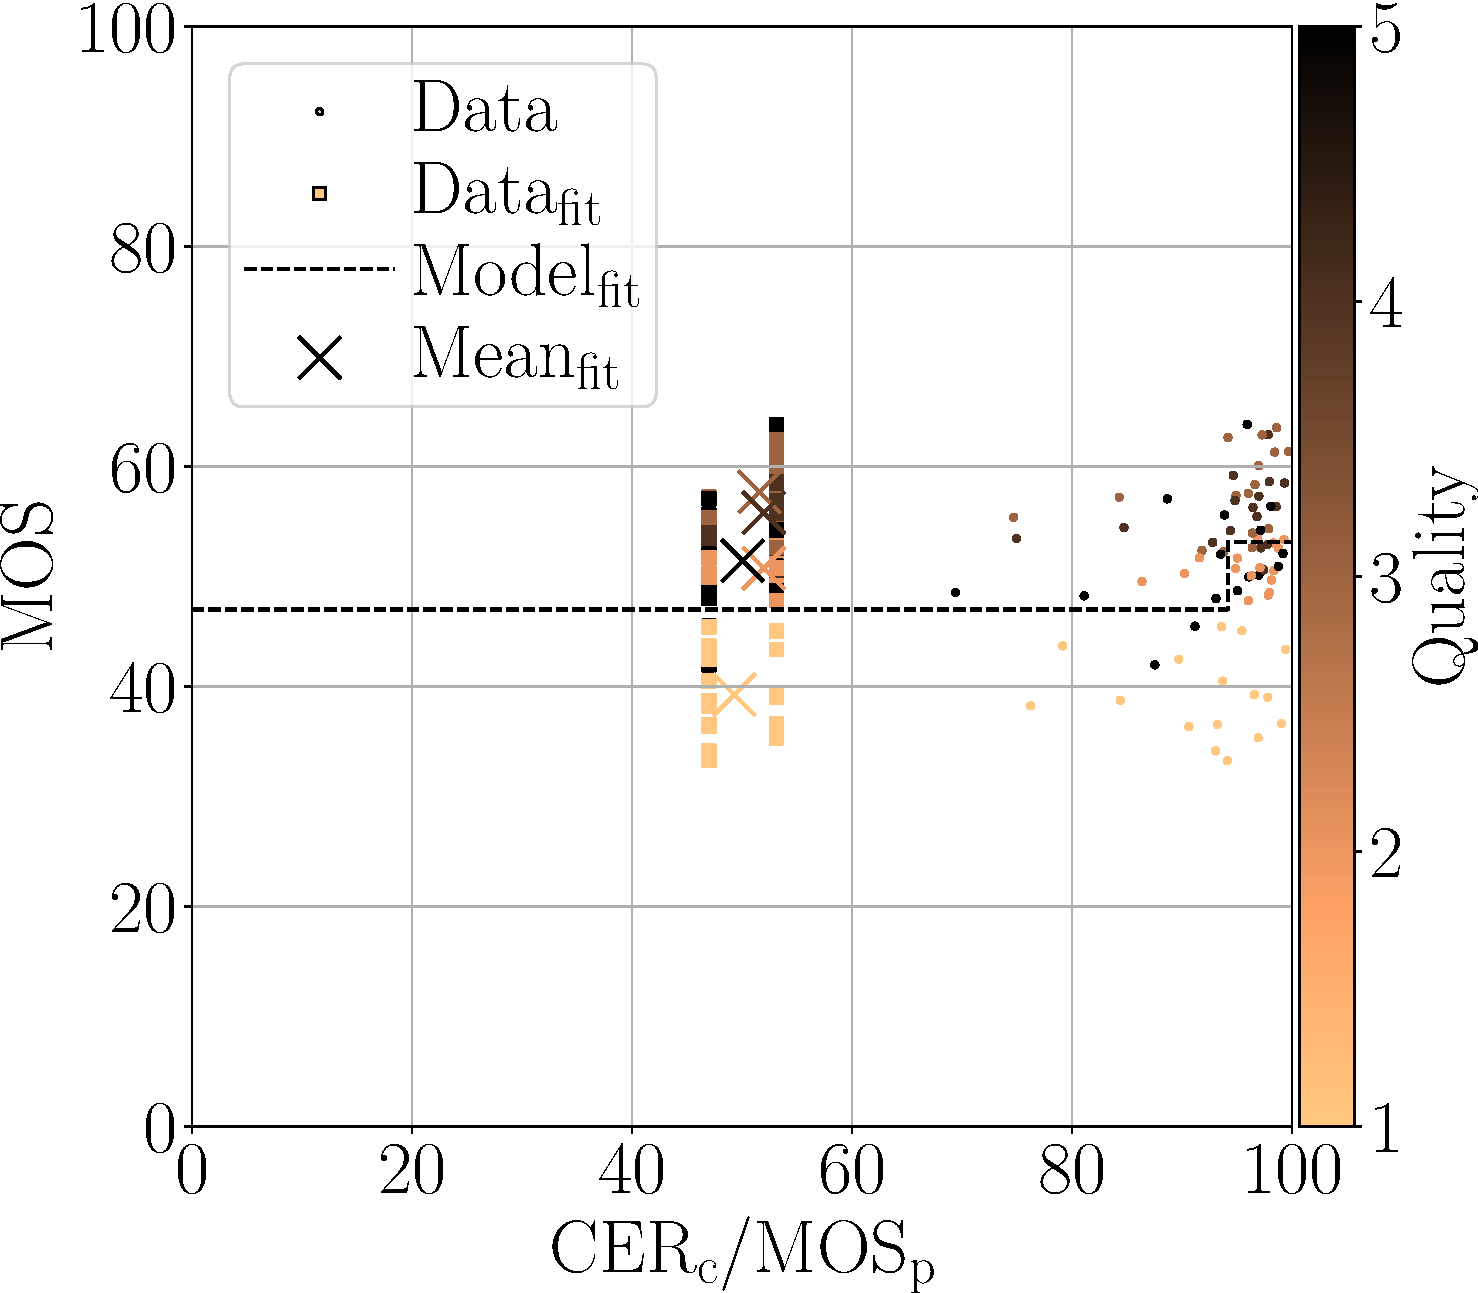
\includegraphics[width=\textwidth]{../../images/analyze/mos_cer_ref_fitted_mean_ezocr_CC.pdf}
        \caption{CC}
        \label{fig:mos_cer_ref_fitted_mean_ezocr_CC}
    \end{subfigure}
    \hfill
    \begin{subfigure}[b]{0.3\textwidth}
        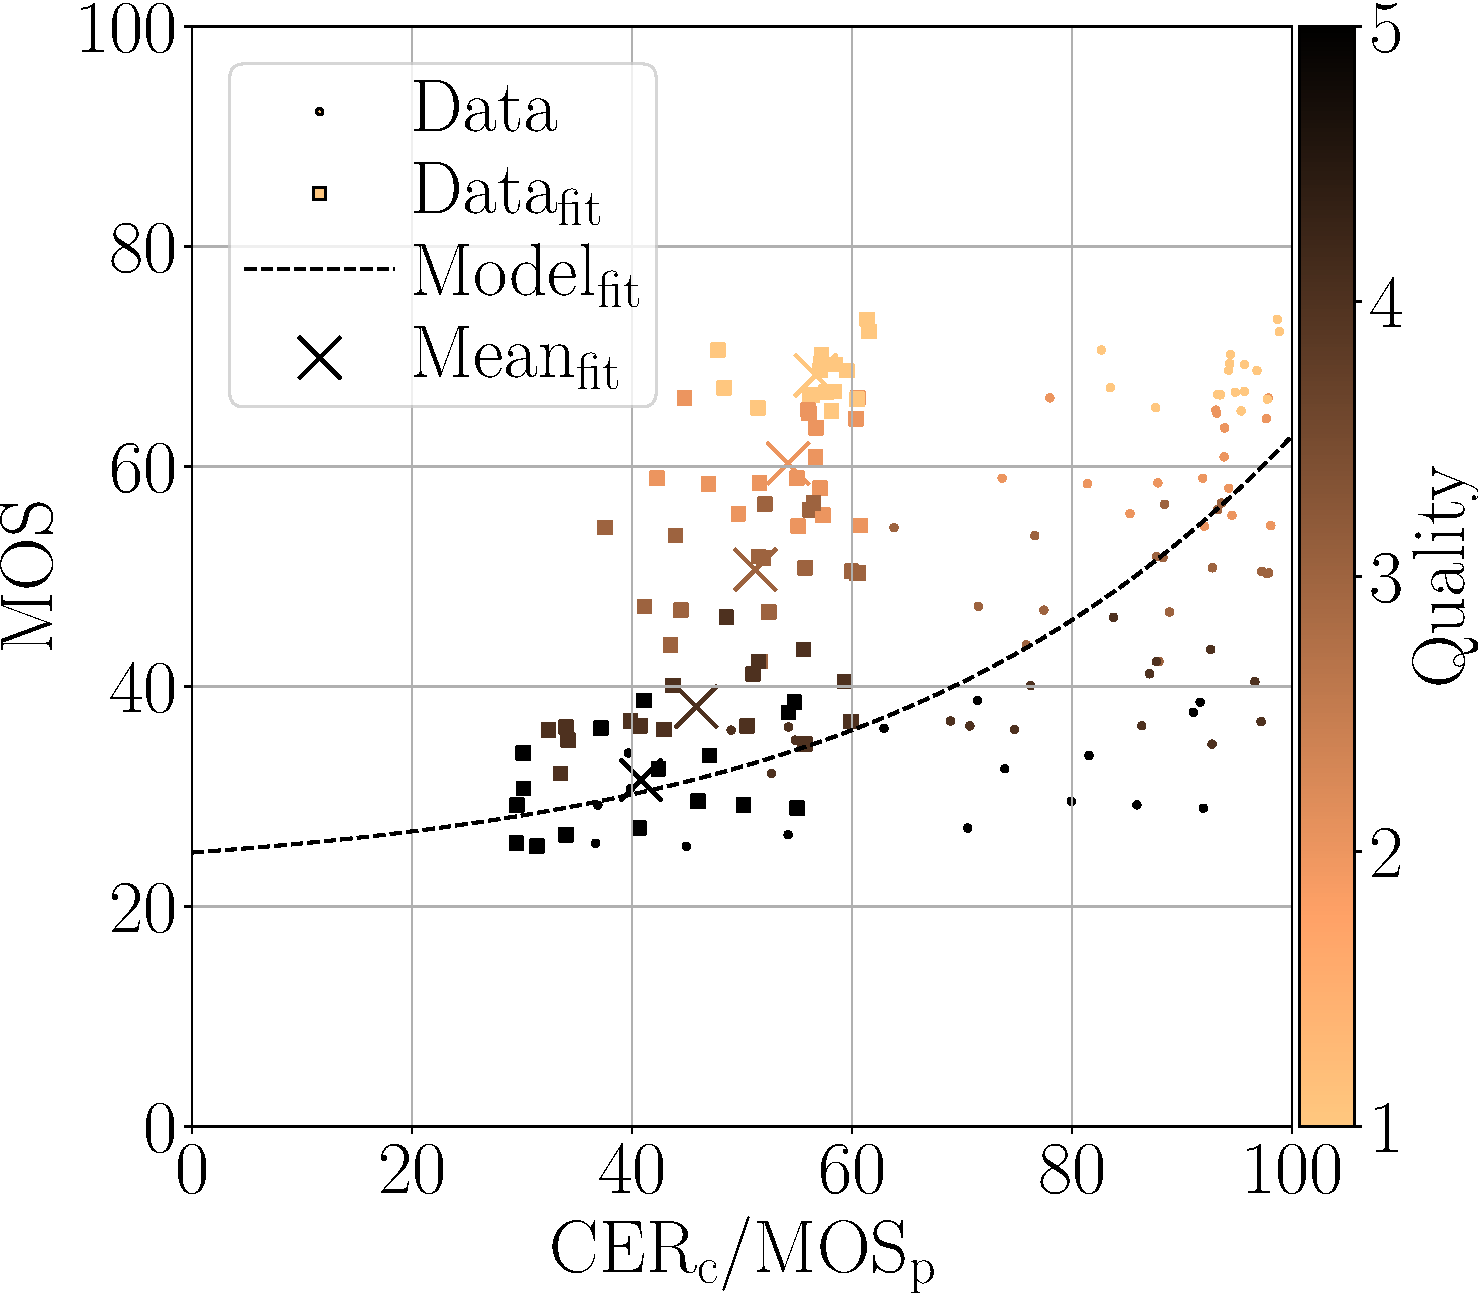
\includegraphics[width=\textwidth]{../../images/analyze/mos_cer_ref_fitted_mean_ezocr_JPEG.pdf}
        \caption{JPEG}
        \label{fig:mos_cer_ref_fitted_mean_ezocr_JPEG}
    \end{subfigure}
    \hfill
    \begin{subfigure}[b]{0.3\textwidth}
        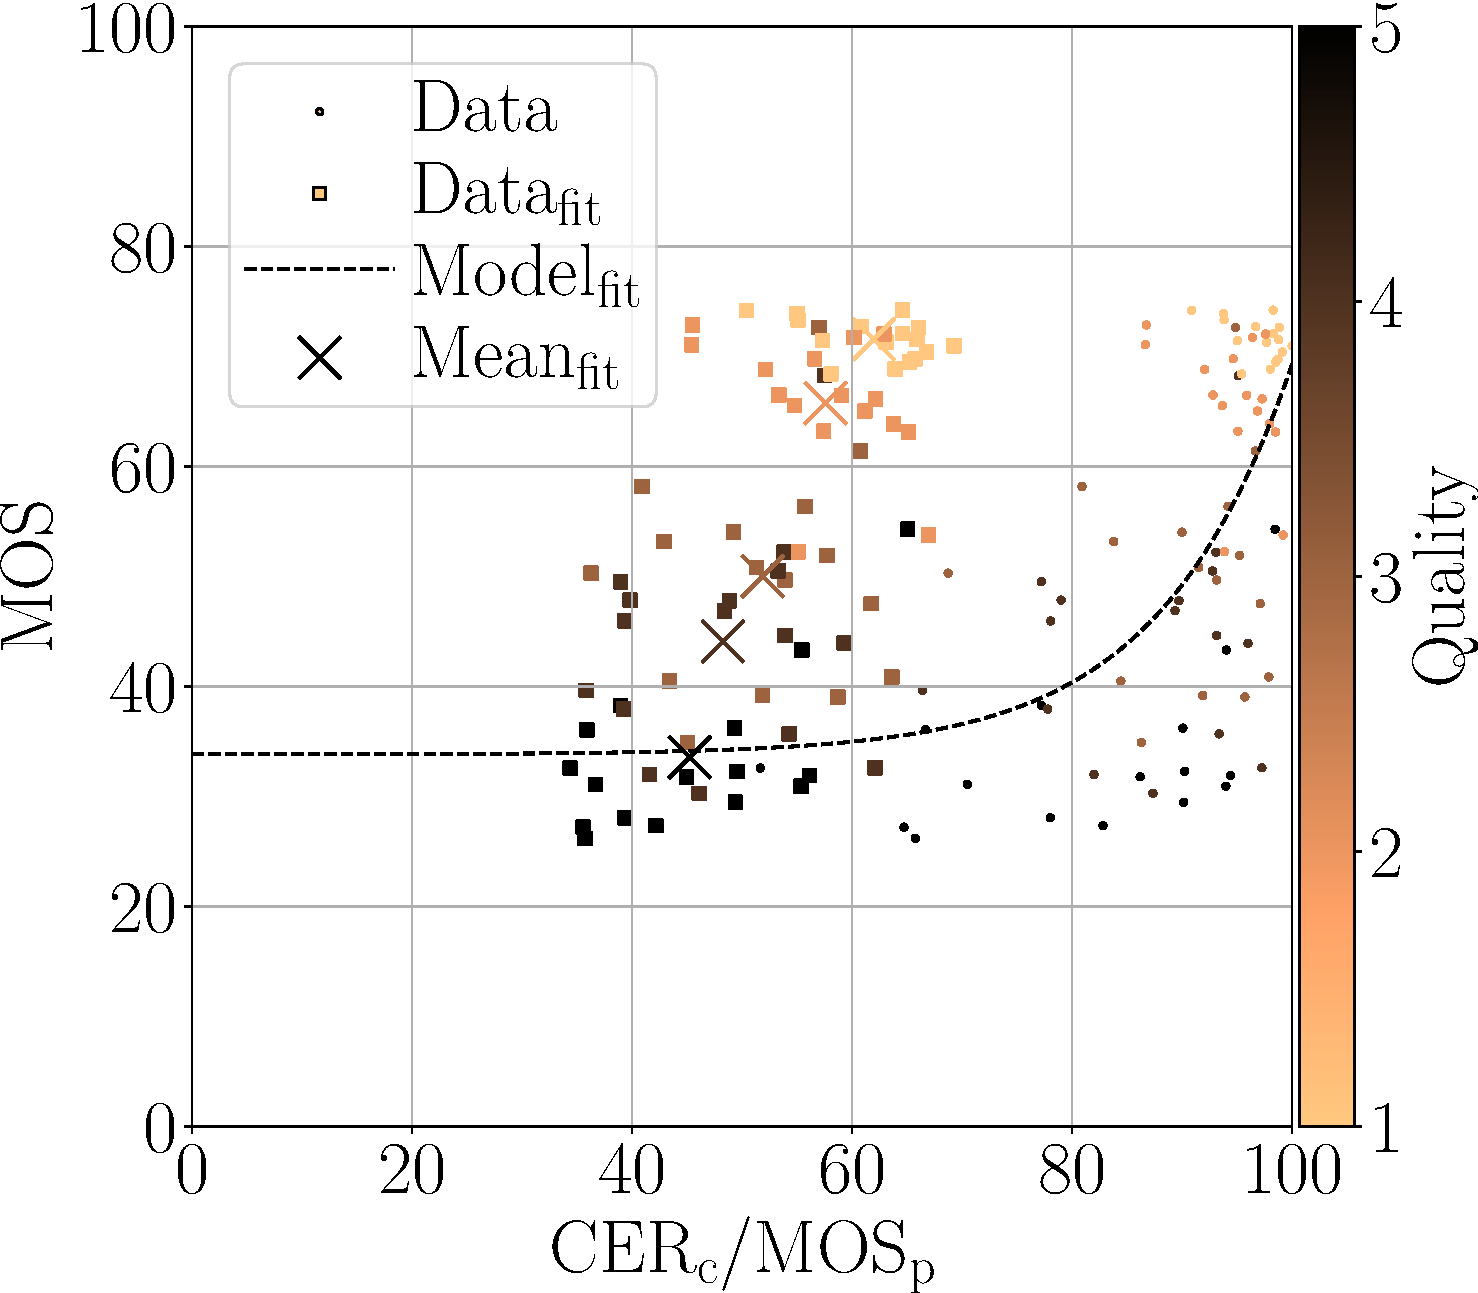
\includegraphics[width=\textwidth]{../../images/analyze/mos_cer_ref_fitted_mean_ezocr_JPEG2000.pdf}
        \caption{JPEG2000}
        \label{fig:mos_cer_ref_fitted_mean_ezocr_JPEG2000}
    \end{subfigure}
    \newline
    \begin{subfigure}[b]{0.3\textwidth}
        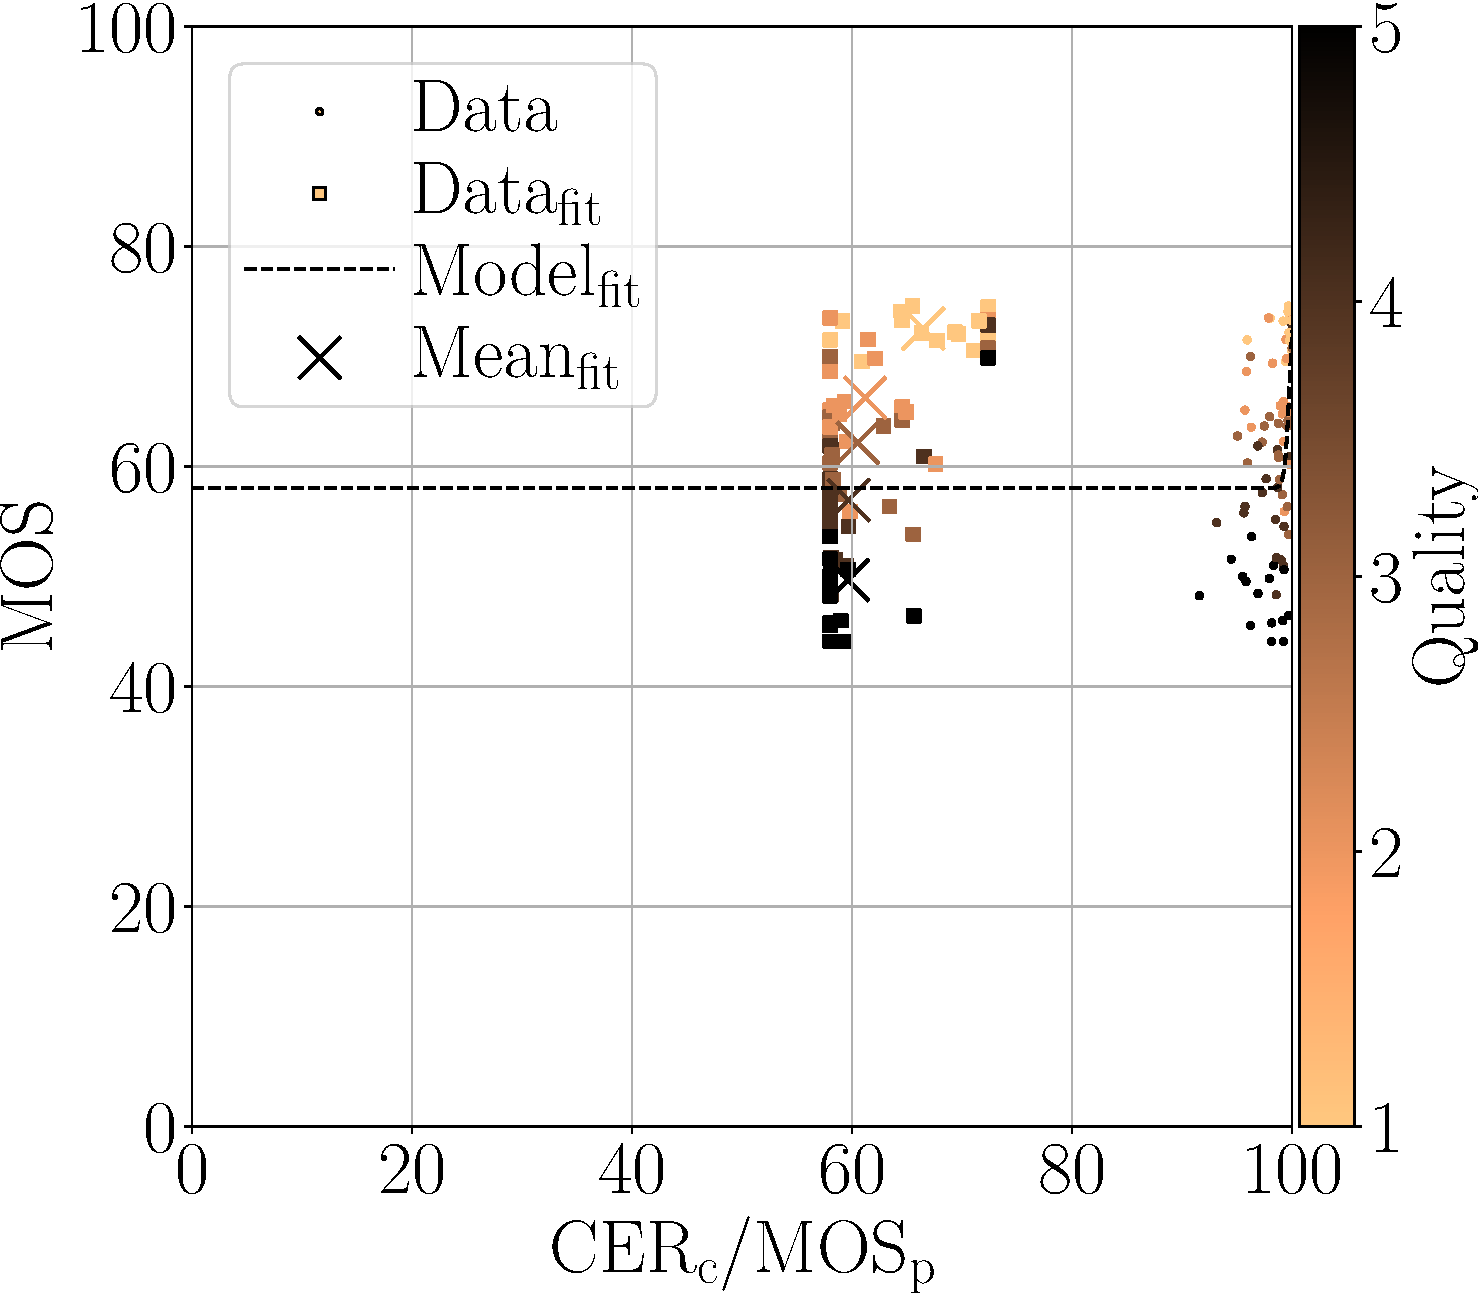
\includegraphics[width=\textwidth]{../../images/analyze/mos_cer_ref_fitted_mean_ezocr_CSC.pdf}
        \caption{CSC}
        \label{fig:mos_cer_ref_fitted_mean_ezocr_CSC}
    \end{subfigure}
    \hfill
    \begin{subfigure}[b]{0.3\textwidth}
        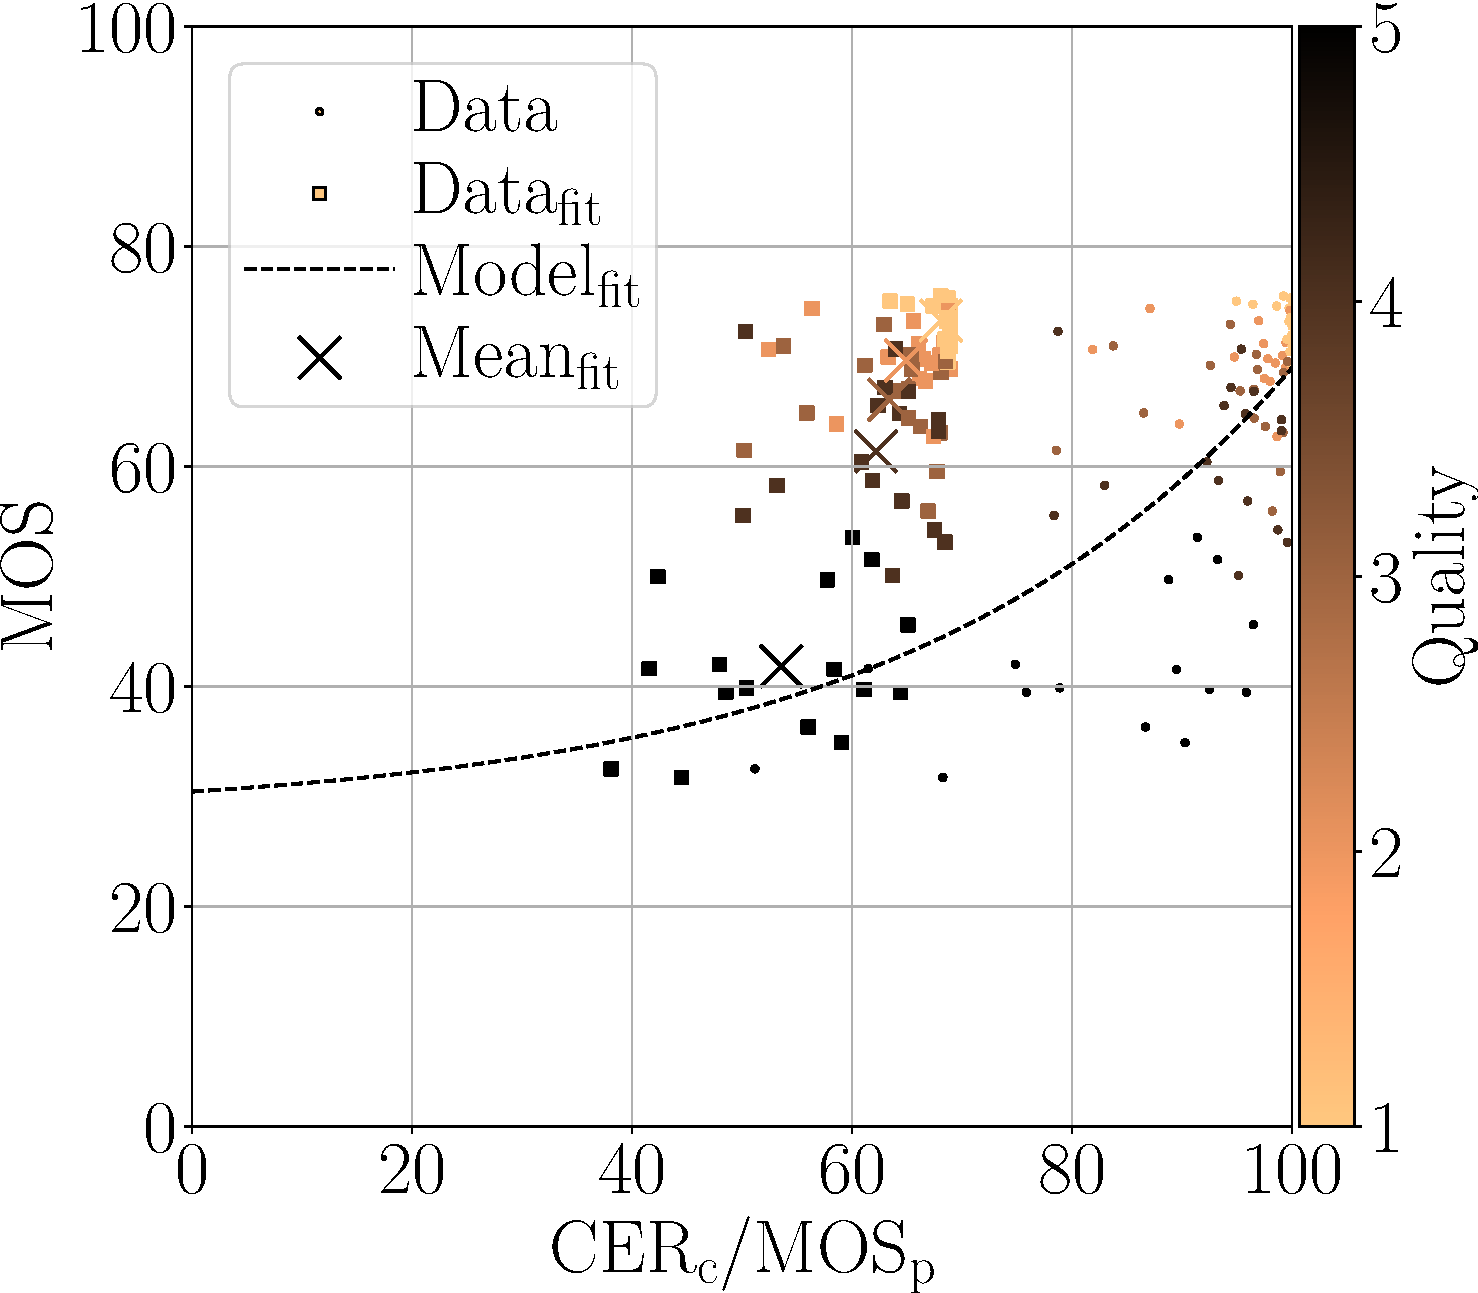
\includegraphics[width=\textwidth]{../../images/analyze/mos_cer_ref_fitted_mean_ezocr_HEVC-SCC.pdf}
        \caption{HEVC-SCC}
        \label{fig:mos_cer_ref_fitted_mean_ezocr_HEVC-SCC}
    \end{subfigure}
    \hfill
    \begin{subfigure}[b]{0.3\textwidth}
        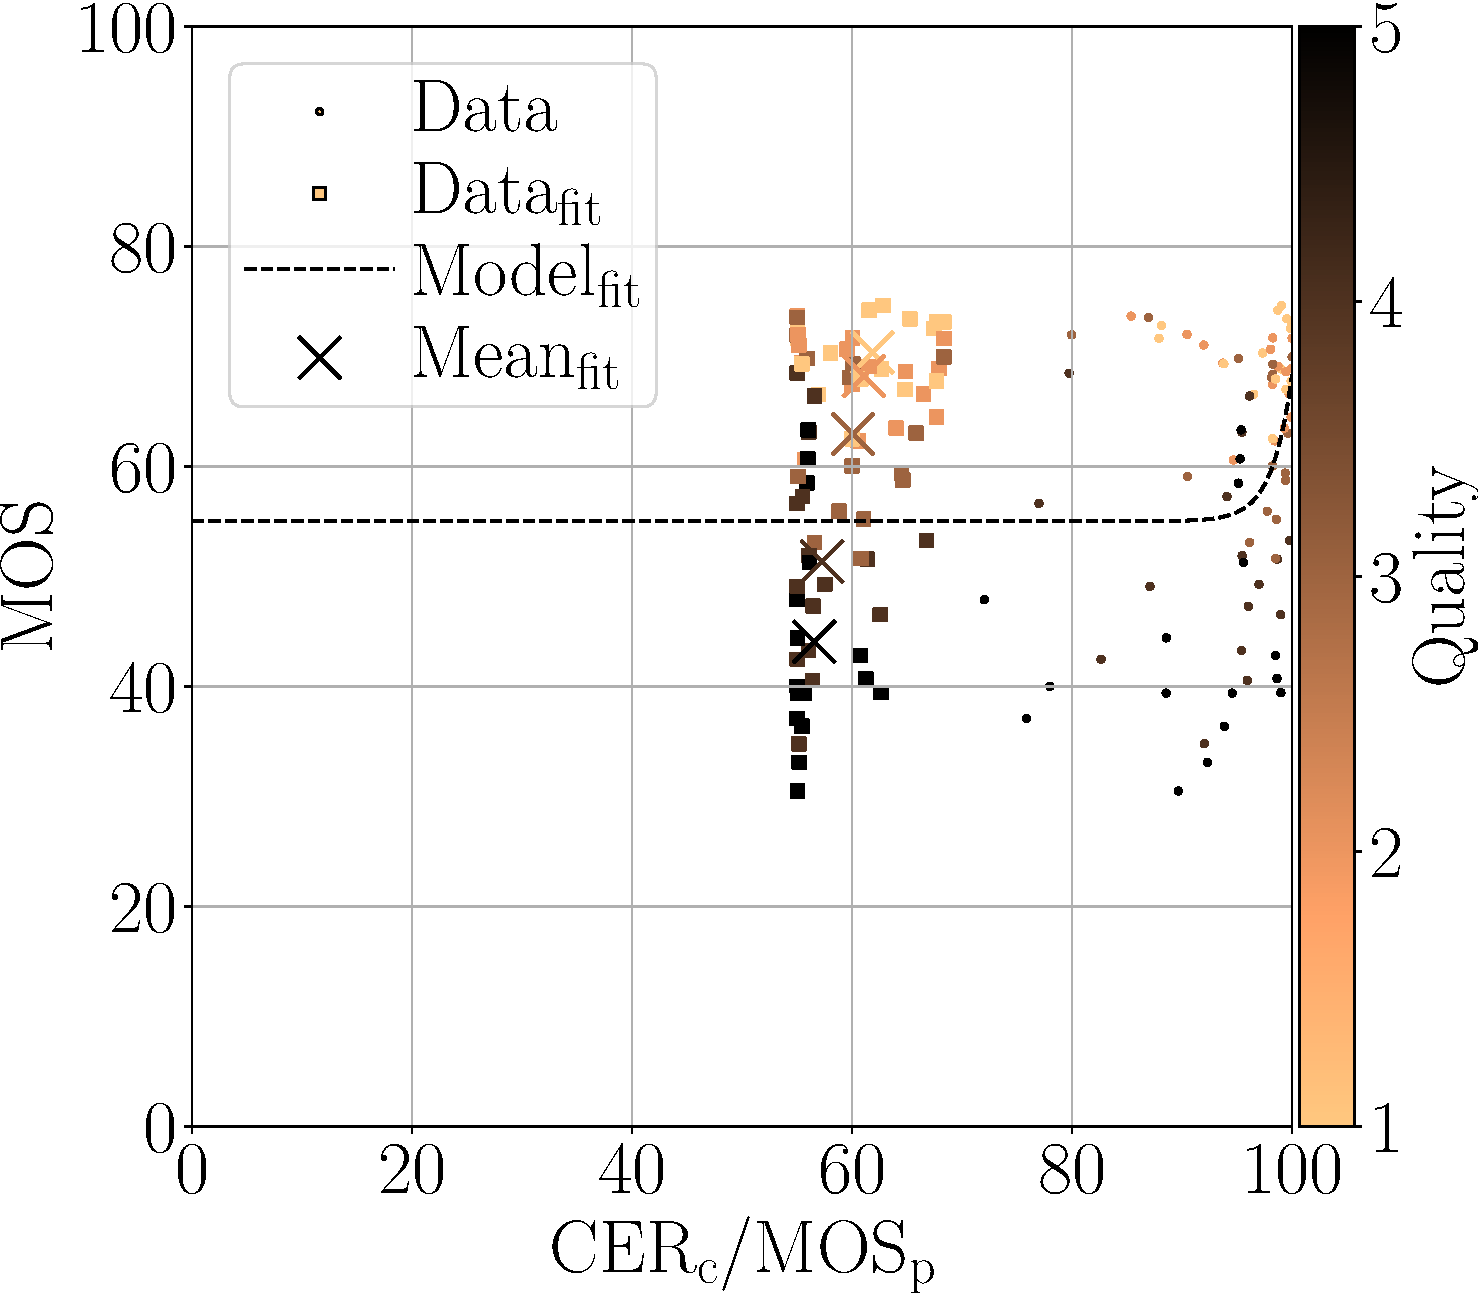
\includegraphics[width=\textwidth]{../../images/analyze/mos_cer_ref_fitted_mean_ezocr_CQD.pdf}
        \caption{CQD}
        \label{fig:mos_cer_ref_fitted_mean_ezocr_CQD}
    \end{subfigure}
    \caption{Mean $\text{CER}_{\text{c}}$ (fitted) in relation to the reference against mean \gls{mos} for different distortion types with EasyOCR.}
\label{fig:mos_cer_ref_fitted_mean_ezocr}
\end{figure}

In \autoref{fig:mos_cer_ref_fitted_mean_ezocr} we can see the mean $\text{CER}_{\text{c}}$ (fitted) against the mean \gls{mos} over selected images for all distortions with EasyOCR.

% mos vs cer (fitted) mean in relation to reference for Tesseract
\begin{figure}[h]
\centering
    \begin{subfigure}[b]{0.3\textwidth}
        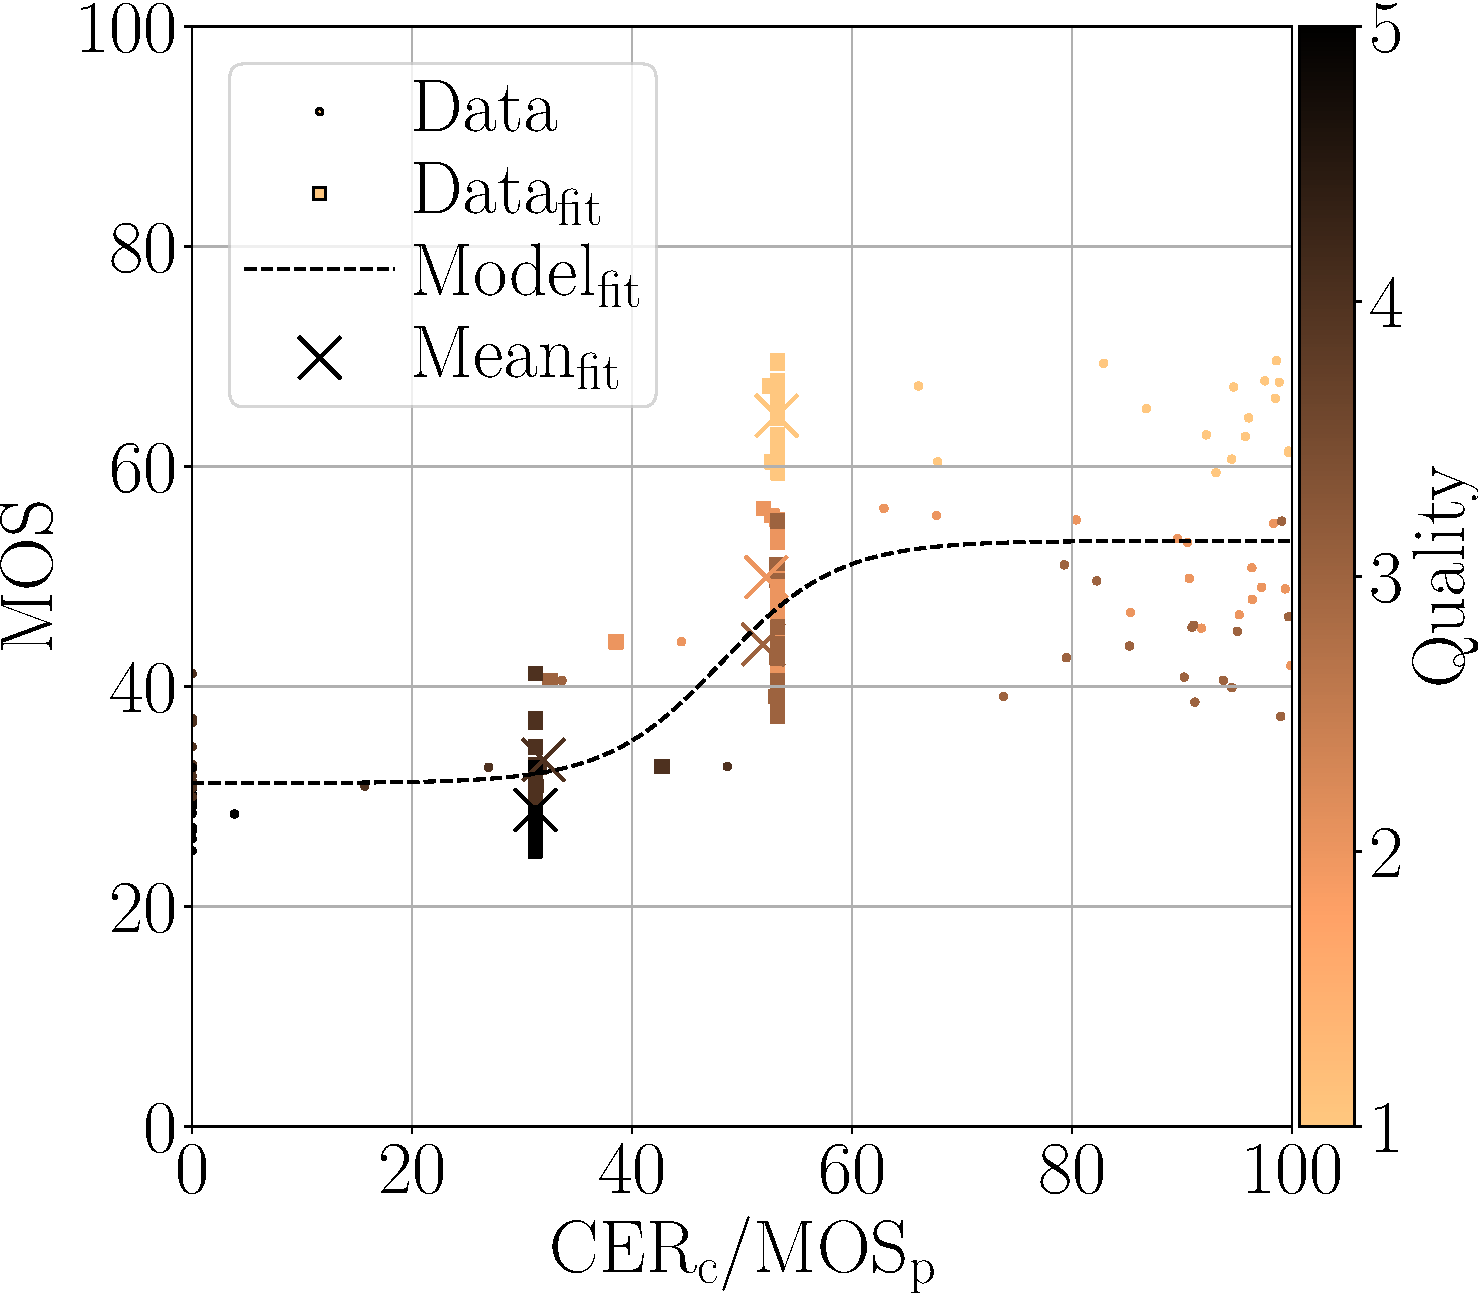
\includegraphics[width=\textwidth]{../../images/analyze/mos_cer_ref_fitted_mean_tess_GN.pdf}
        \caption{GN}
        \label{fig:mos_cer_ref_fitted_mean_tess_GN}
    \end{subfigure}
    \hfill
    \begin{subfigure}[b]{0.3\textwidth}
        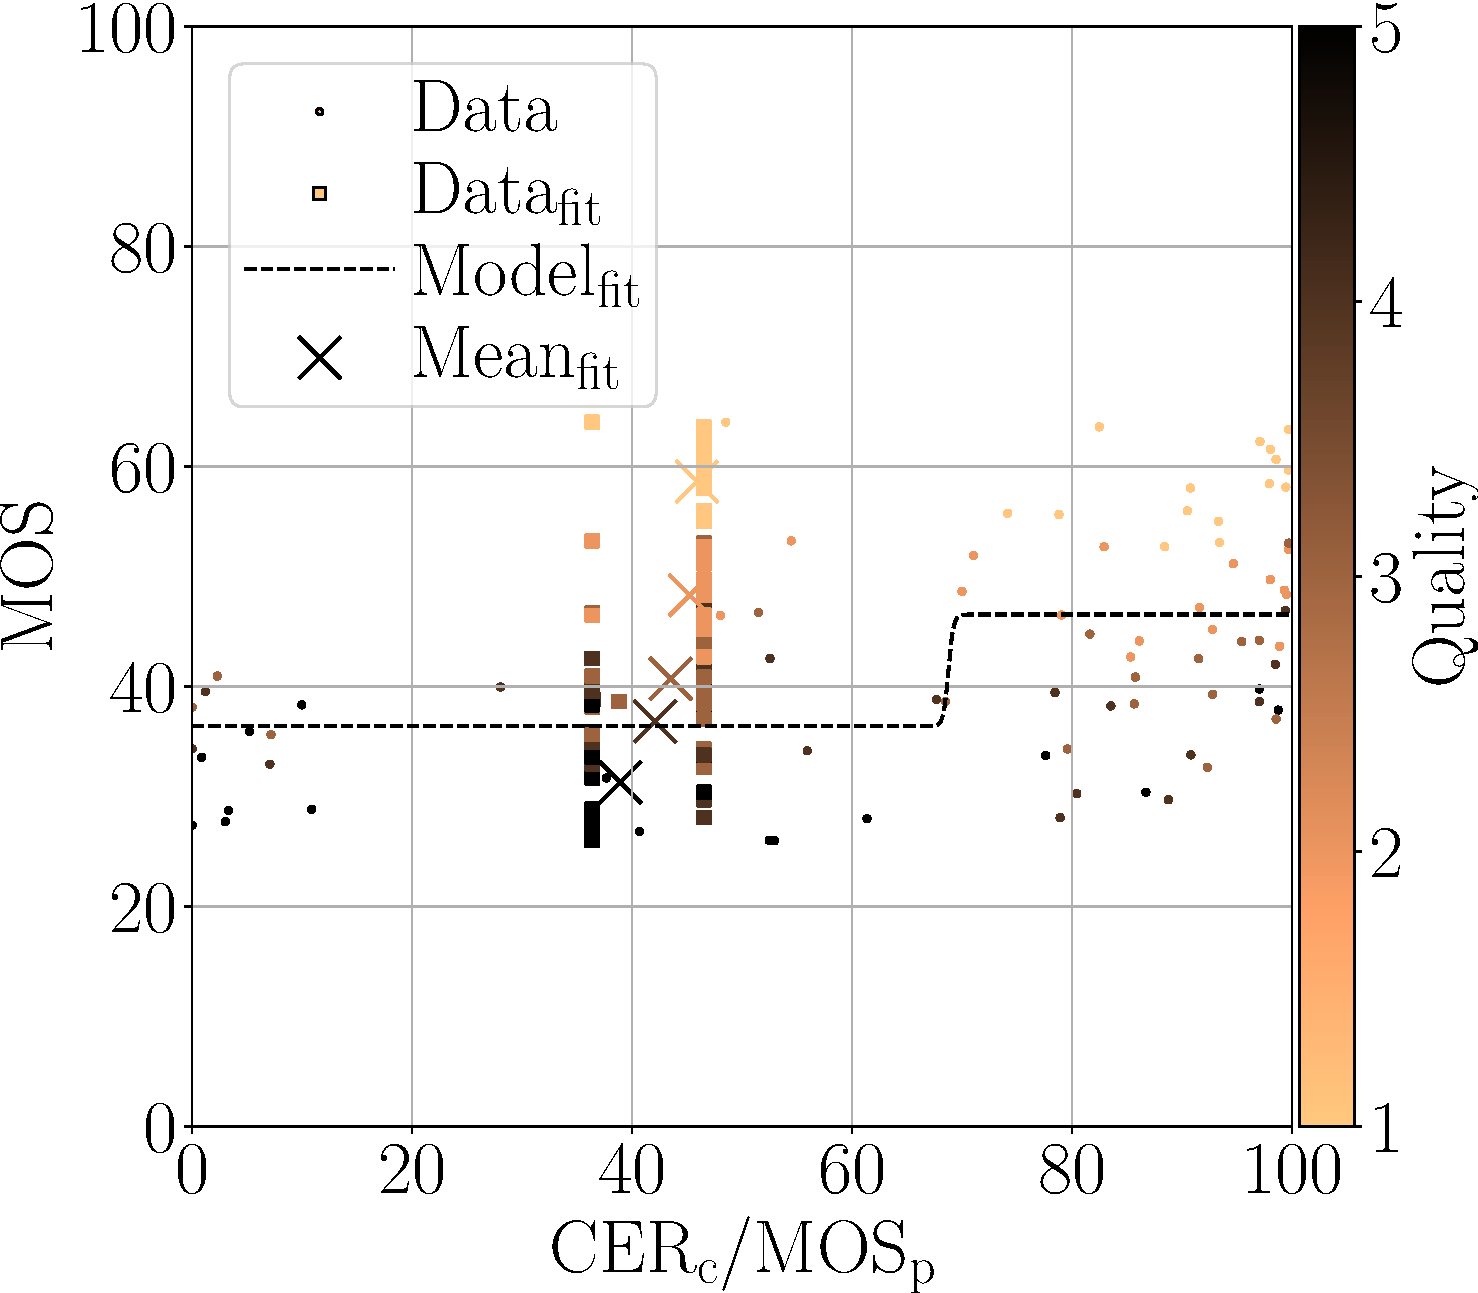
\includegraphics[width=\textwidth]{../../images/analyze/mos_cer_ref_fitted_mean_tess_GB.pdf}
        \caption{GB}
        \label{fig:mos_cer_ref_fitted_mean_tess_GB}
    \end{subfigure}
    \hfill
    \begin{subfigure}[b]{0.3\textwidth}
        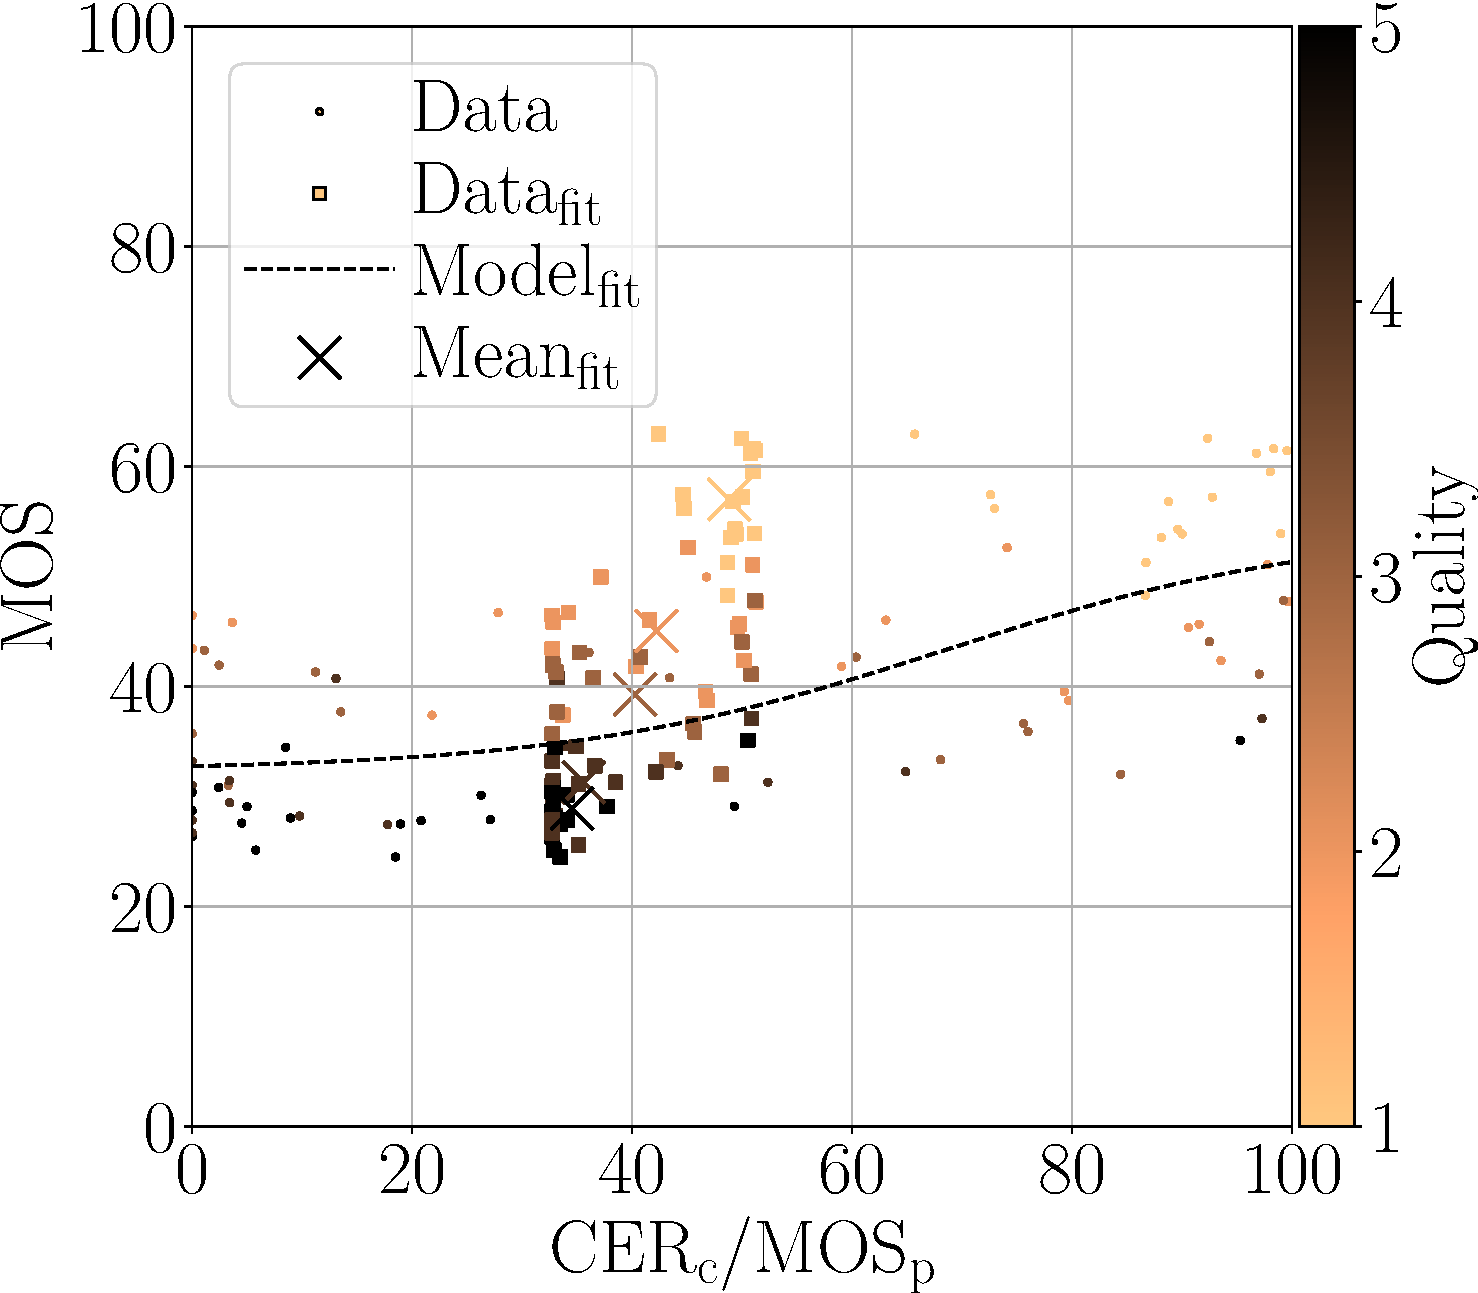
\includegraphics[width=\textwidth]{../../images/analyze/mos_cer_ref_fitted_mean_tess_MB.pdf}
        \caption{MB}
        \label{fig:mos_cer_ref_fitted_mean_tess_MB}
    \end{subfigure}
    \newline
    \begin{subfigure}[b]{0.3\textwidth}
        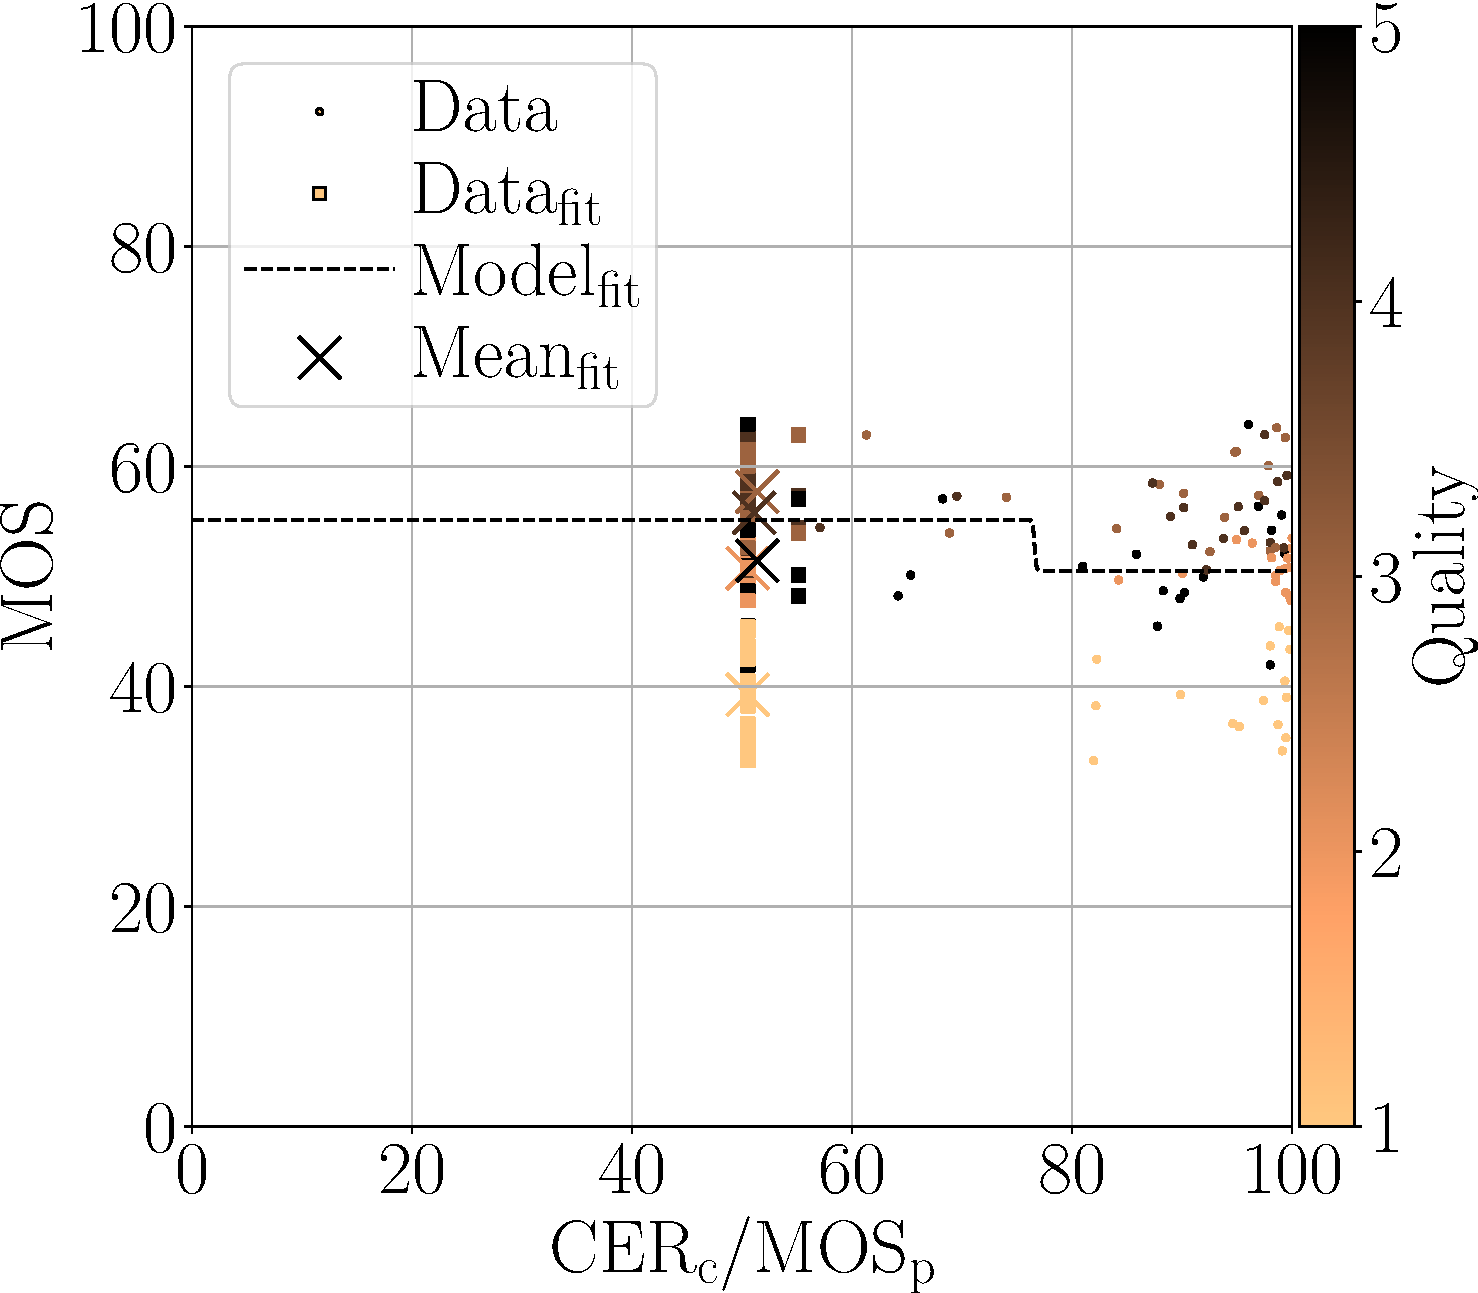
\includegraphics[width=\textwidth]{../../images/analyze/mos_cer_ref_fitted_mean_tess_CC.pdf}
        \caption{CC}
        \label{fig:mos_cer_ref_fitted_mean_tess_CC}
    \end{subfigure}
    \hfill
    \begin{subfigure}[b]{0.3\textwidth}
        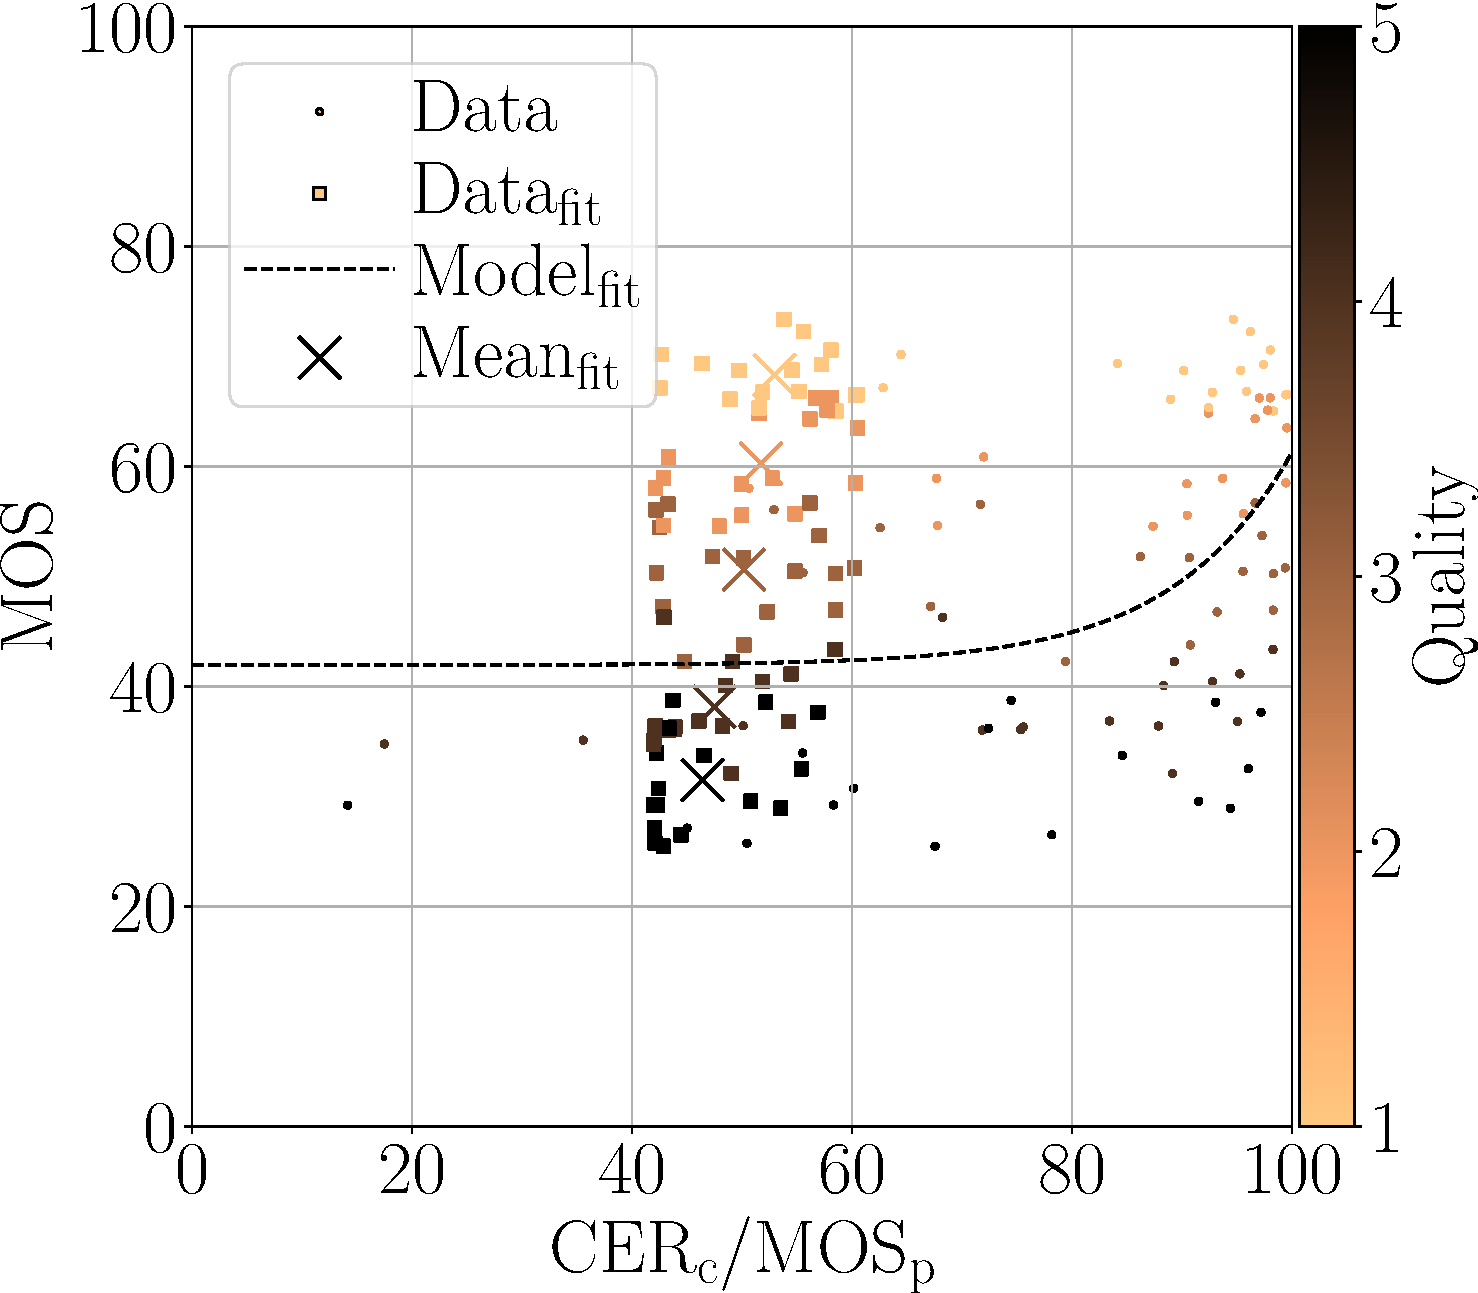
\includegraphics[width=\textwidth]{../../images/analyze/mos_cer_ref_fitted_mean_tess_JPEG.pdf}
        \caption{JPEG}
        \label{fig:mos_cer_ref_fitted_mean_tess_JPEG}
    \end{subfigure}
    \hfill
    \begin{subfigure}[b]{0.3\textwidth}
        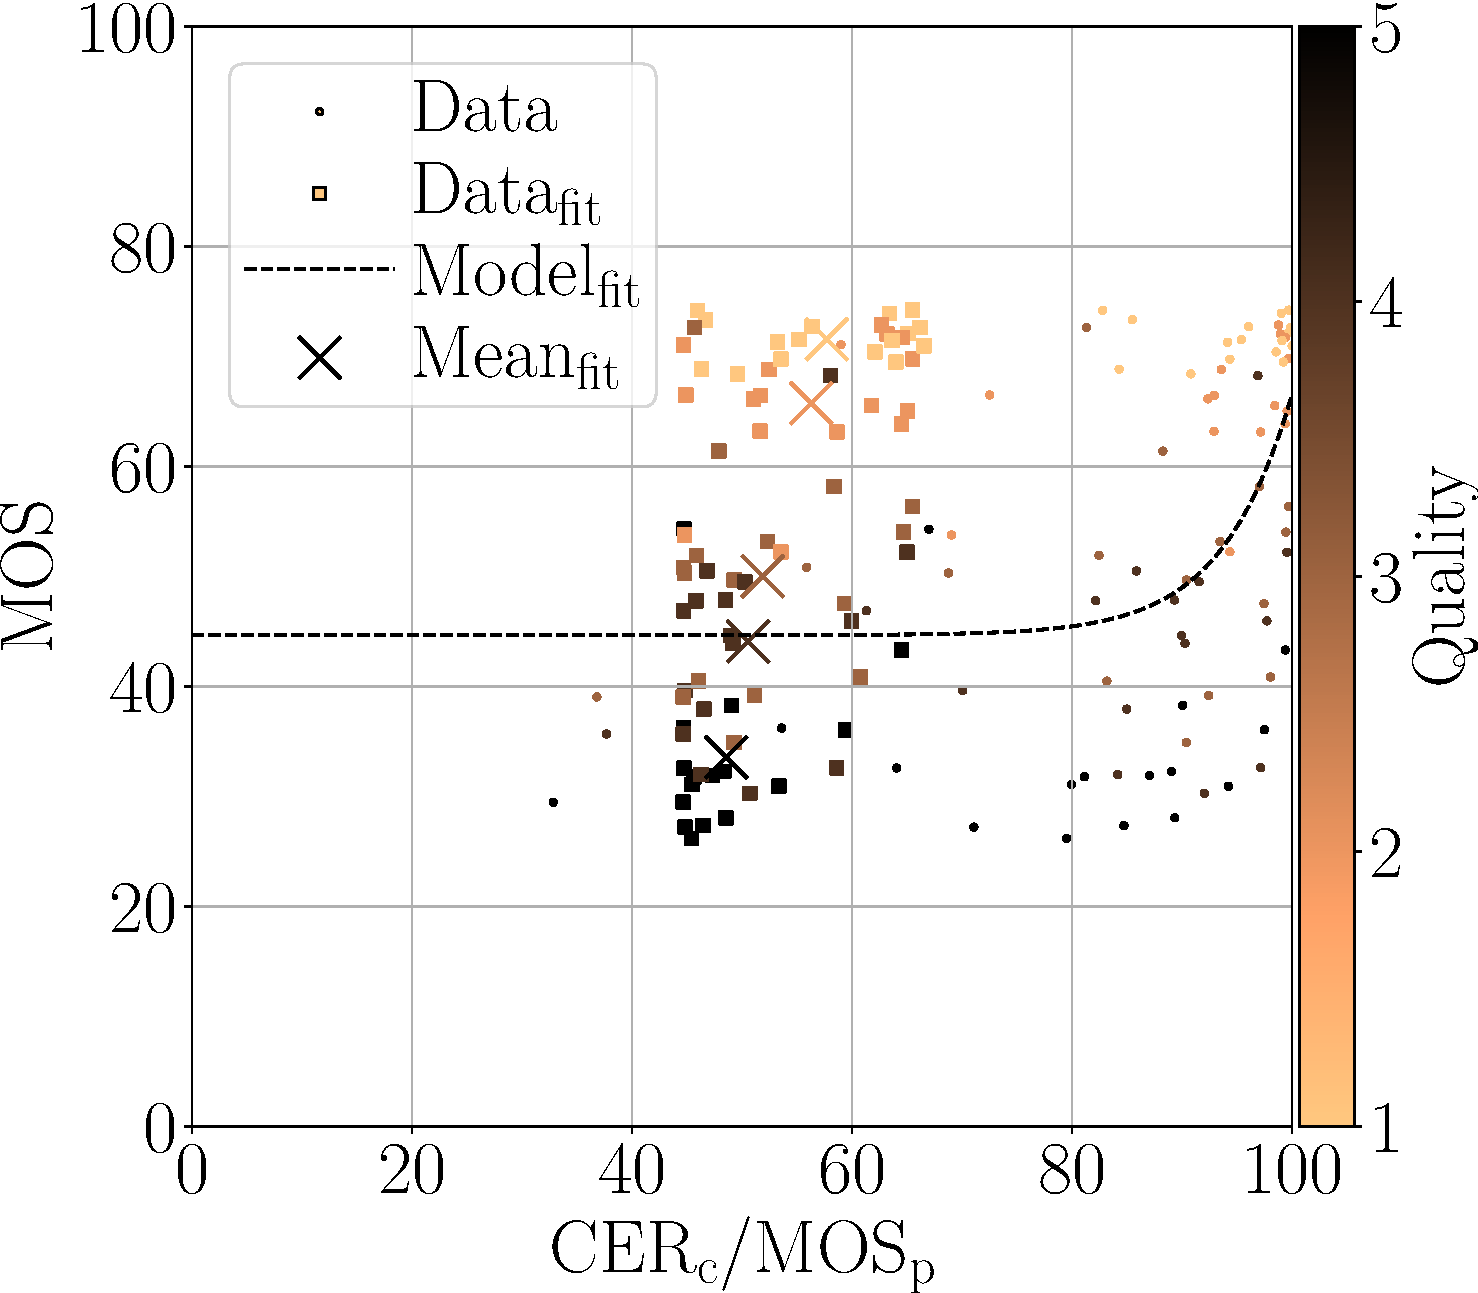
\includegraphics[width=\textwidth]{../../images/analyze/mos_cer_ref_fitted_mean_tess_JPEG2000.pdf}
        \caption{JPEG2000}
        \label{fig:mos_cer_ref_fitted_mean_tess_JPEG2000}
    \end{subfigure}
    \newline
    \begin{subfigure}[b]{0.3\textwidth}
        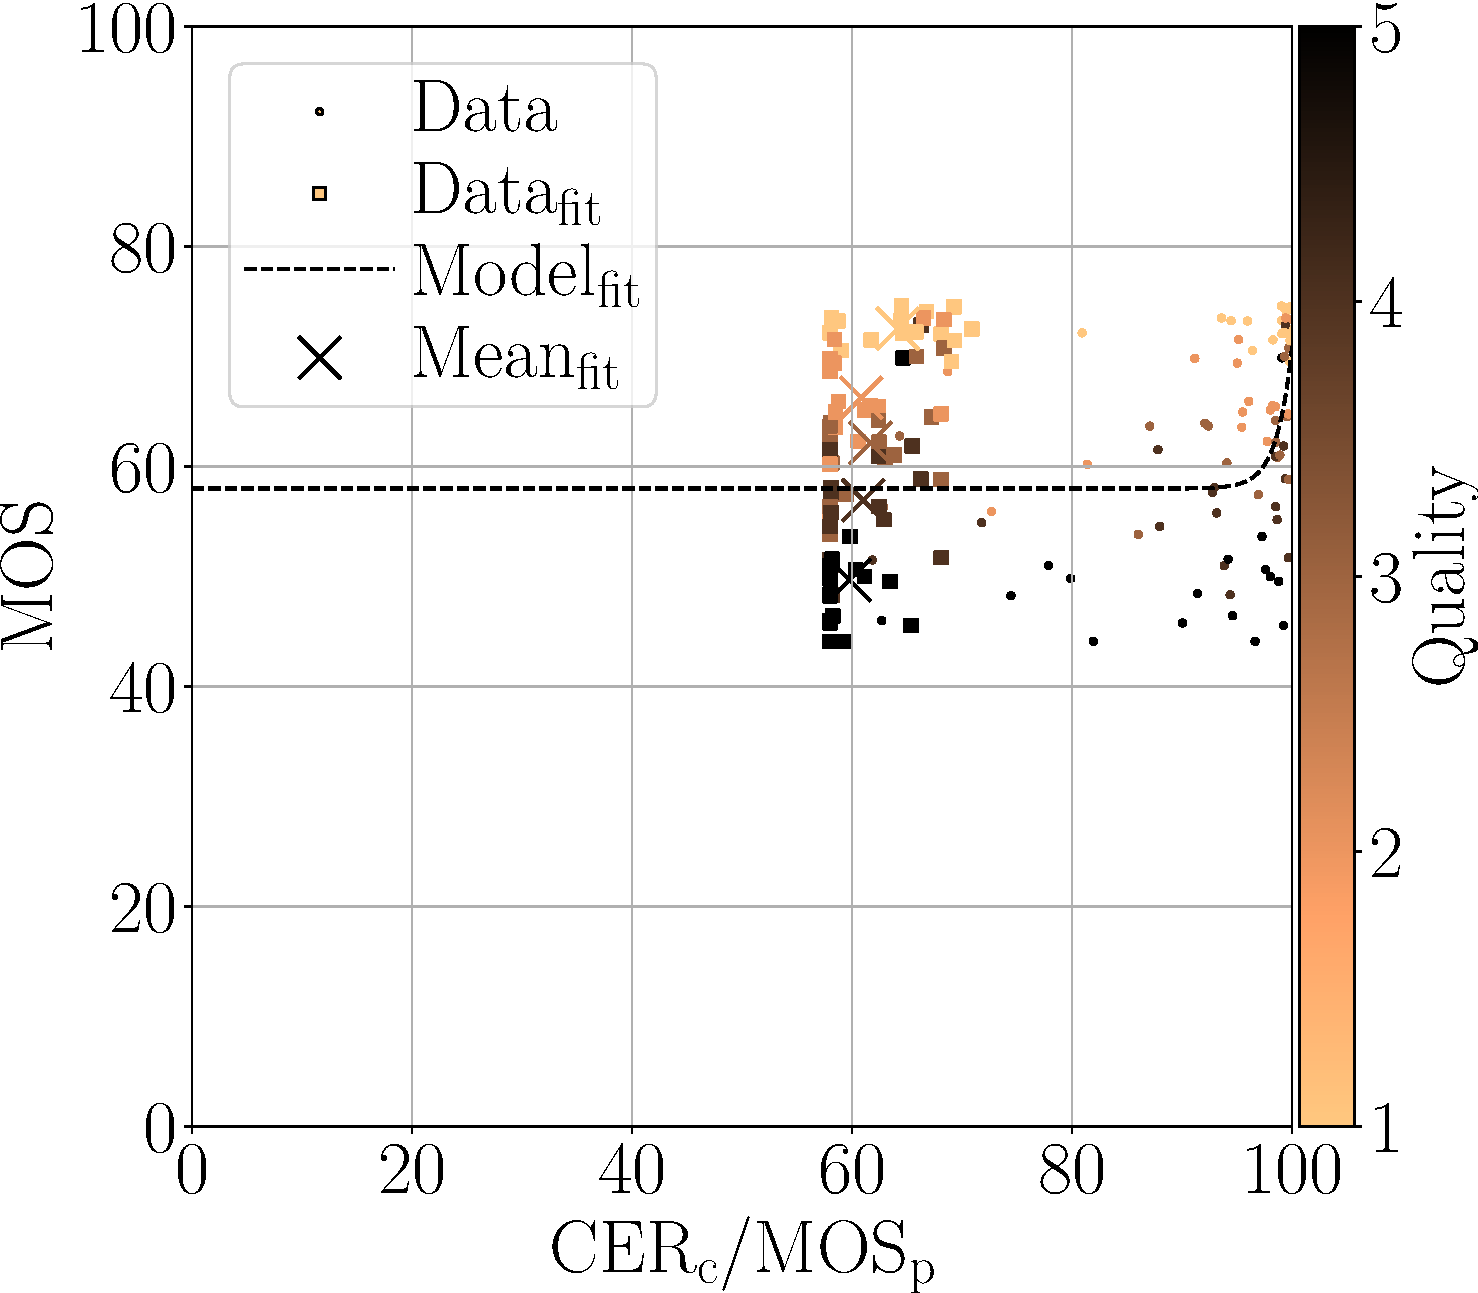
\includegraphics[width=\textwidth]{../../images/analyze/mos_cer_ref_fitted_mean_tess_CSC.pdf}
        \caption{CSC}
        \label{fig:mos_cer_ref_fitted_mean_tess_CSC}
    \end{subfigure}
    \hfill
    \begin{subfigure}[b]{0.3\textwidth}
        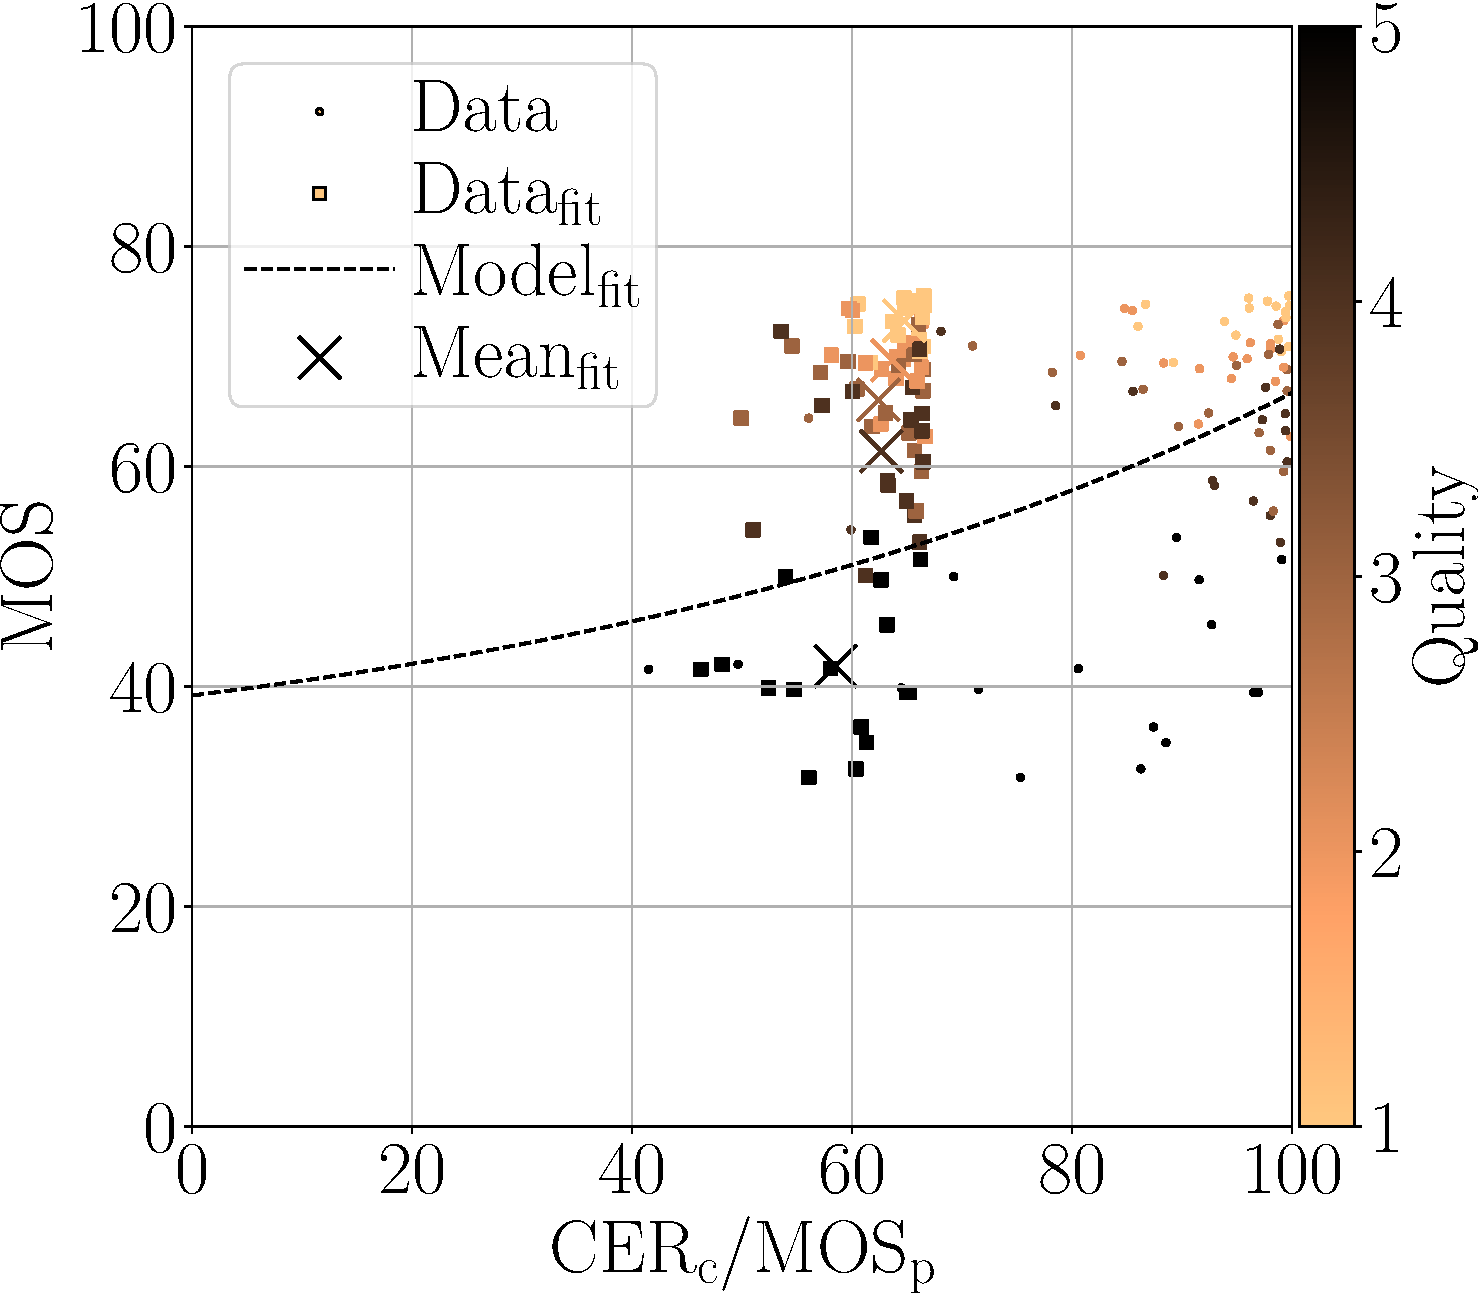
\includegraphics[width=\textwidth]{../../images/analyze/mos_cer_ref_fitted_mean_tess_HEVC-SCC.pdf}
        \caption{HEVC-SCC}
        \label{fig:mos_cer_ref_fitted_mean_tess_HEVC-SCC}
    \end{subfigure}
    \hfill
    \begin{subfigure}[b]{0.3\textwidth}
        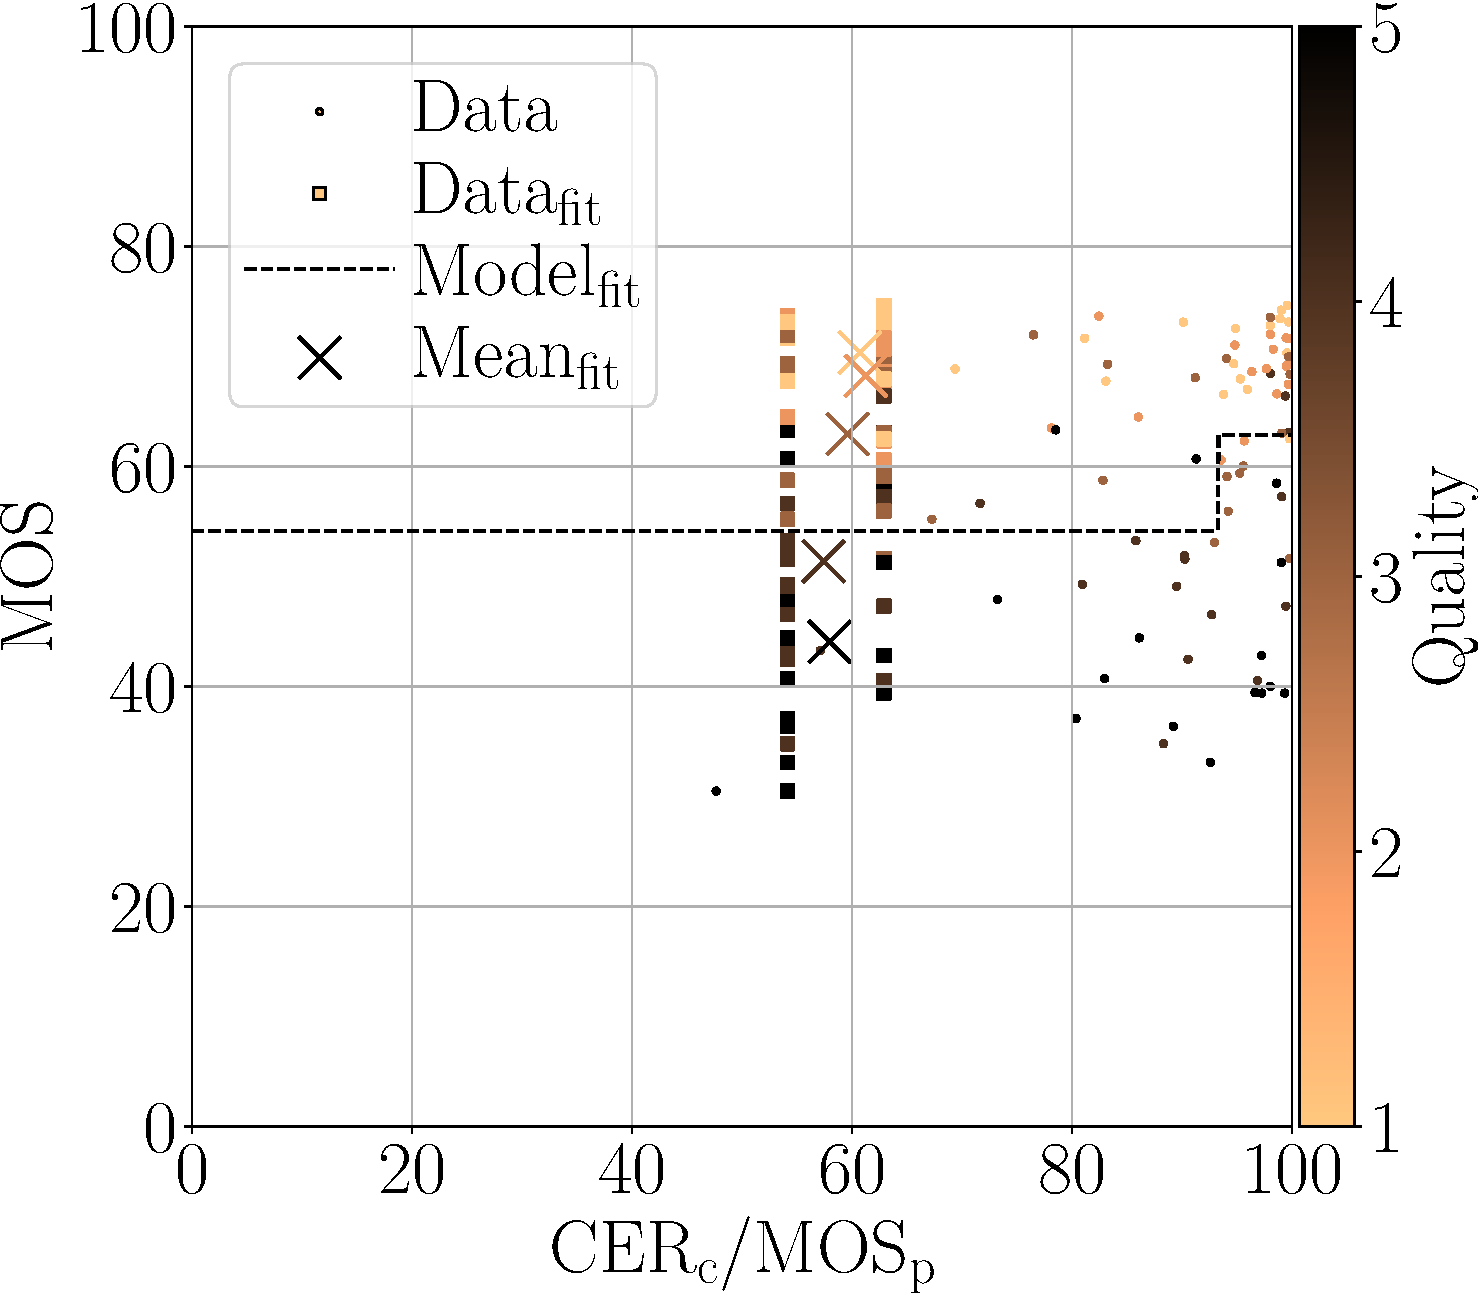
\includegraphics[width=\textwidth]{../../images/analyze/mos_cer_ref_fitted_mean_tess_CQD.pdf}
        \caption{CQD}
        \label{fig:mos_cer_ref_fitted_mean_tess_CQD}
    \end{subfigure}
    \caption{Mean $\text{CER}_{\text{c}}$ (fitted) in relation to the reference against mean \gls{mos} for different distortion types with Tesseract \gls{ocr}.}
\label{fig:mos_cer_ref_fitted_mean_tess}
\end{figure}

In \autoref{fig:mos_cer_ref_fitted_mean_tess} we can see the mean $\text{CER}_{\text{c}}$ (fitted) against the mean \gls{mos} over selected images for all distortions with Tesseract \gls{ocr}.


\begin{table}[h]
    \centering
    \begin{tabular}{|l|rrr|}
        \hline
        Distortion Type & SRCC & PLCC & RMSE \\
        \hline
        CC & 0.29 & 0.40 & 6.76 \\
        CQD & 0.28 & 0.36 & 11.45 \\
        CSC & 0.47 & 0.54 & 7.65 \\
        GB & 0.70 & 0.71 & 7.40 \\
        GN & 0.56 & 0.54 & 11.09 \\
        HEVC-SCC & 0.57 & 0.62 & 9.42 \\
        JPEG & 0.65 & 0.66 & 10.65 \\
        JPEG2000 & 0.59 & 0.61 & 12.41 \\
        MB & 0.86 & 0.85 & 5.73 \\
        \hline
        Overall & 0.65 & 0.66 & 9.44 \\
        \hline
    \end{tabular}
    \caption{Correlations and RMSE for different distortion types for EasyOCR}
    \label{tab:fitted_metrics_ezocr}
\end{table}

To quantify the observations we calculate the \gls{plcc}, \gls{srcc} and \gls{rmse} as described in \autoref{chap:qualityassessment}.
In \autoref{tab:fitted_metrics_ezocr} we can see metrics for all distortions and for all distortions together (overall) for EasyOCR.


This might be due to the fact that the \gls{ocr} sometimes predicts text where there is no text or the \gls{gt} does not contain that text.
Thus when the quality gets worse, it might happen, that those text elements do not get predicted at all, thus resulting in a better performance.
The correlation is affected because the $\text{CER}_{\text{c}}$ first goes up and then down again, but the \gls{mos} is strictly decreasing.

The \gls{plcc} is generally higher for EasyOCR than for Tesseract \gls{ocr}.
This suggests that EasyOCR is more similarly to humans than Tesseract \gls{ocr} with regard to the impact on the $\text{CER}_{\text{c}}$ by the distortions.
Additionally the lowest \gls{plcc} is seen for \gls{cc}, which further confirms our assumption that \gls{cc} is not really an impact for the \gls{ocr} and thus not correlated with the \gls{mos}.
Similar observations, although more dominant for \gls{srcc}, can be made for \gls{csc} and \gls{cqd}.
These two distortions also seem to have more impact on the \gls{mos} than on the \gls{ocr} algorithms, which makes sense.

\begin{table}[h]
    \centering
    \begin{tabular}{|l|rrr|}
        \hline
        Distortion Type & SRCC & PLCC & RMSE \\
        \hline
        CC & -0.21 & 0.29 & 7.06 \\
        CQD & 0.33 & 0.42 & 11.16 \\
        CSC & 0.46 & 0.44 & 8.15 \\
        GB & 0.58 & 0.56 & 8.69 \\
        GN & 0.77 & 0.79 & 8.03 \\
        HEVC-SCC & 0.36 & 0.30 & 11.44 \\
        JPEG & 0.49 & 0.55 & 11.82 \\
        JPEG2000 & 0.46 & 0.50 & 13.56 \\
        MB & 0.65 & 0.68 & 8.00 \\
        \hline
        Overall & 0.55 & 0.57 & 10.00 \\
        \hline
    \end{tabular}
    \caption{Correlations and RMSE for different distortion types for Tesseract \gls{ocr}}
    \label{tab:fitted_metrics_tess}
\end{table}

In \autoref{tab:pearson_spear} we can see the correlation between the $\text{CER}_{\text{c}}$, in relation to the \gls{gt} and the reference, and the now fitted \gls{mos} values for all distortions with EasyOCR and Tesseract \gls{ocr}.
After fitting the \gls{mos} values, we can observe that the correlations increased across the whole table.
This is to be expected, since most of the fitted models are monotonic functions, which makes a higher $\text{CER}_{\text{c}}$ always result in a higher \gls{mos} or vice versa, when going along the model's curve.
The only exception is \gls{cc}, which shows a negative \gls{plcc} and \gls{srcc}.
This is due to a strictly decreasing fitted model as can be seen in \autoref{fig:mos_cer_ref_fitted_mean_tess_CC}.

In summary, we can say that the \gls{gn}, \gls{mb}, \gls{gb}, \gls{jpeg} and \gls{jpeg2000} distortions have a high correlation with the \gls{mos} and \gls{ocr} might be a useful alternative to human judgment.
However, for \gls{cc}, \gls{csc} and \gls{cqd} the correlation with the \gls{mos} is low and \gls{ocr} might not be a good alternative to human judgment.
So one always needs to determine if the distortion is impacting the \gls{ocr} algorithm similar to the human judgment.

    
\section{Usage of Recognized Text as Ground Truth}
\label{sec:usage_of_recognized_text_as_ground_truth}

Since most datasets do not contain textual ground truth information,
in a further step, Mr Hirt will investigate the feasibility of
using recognized text from pristine images as ground truth instead.

\begin{table}[h]
\centering
\begin{tabular}{|c|c|c|}
    \hline
    \rule{0em}{1em} \textbf{OCR Algorithm} & $\mathbf{\overline{CER}}$ & $\mathbf{\overline{CER}_{comp}}$ \\
    \hline
    EasyOCR & 0.16 & 83.79 \\
    \hline
    Tesseract & 0.25 & 75.1 \\
    \hline
\end{tabular}
\caption{Mean $CER$ and $CER_{comp}$ for EasyOCR and Tesseract \gls{ocr} over selected images for reference images against \gls{gt}.}
\label{tab:mean_cer_cer_comp}
\end{table}

From \autoref{tab:mean_cer_cer_comp} we can see that EasyOCR performs better than Tesseract \gls{ocr} on the selected images.
With a $CER_{comp}$ of 83.794 its difficult to recommend using EasyOCR as a ground truth source.
Tesseract is worse with a $CER_{comp}$ of 75.0953, and thus cannot be recommended either.
It might however be possible to improve the performance of the \gls{ocr} algorithms by using a pre-processing pipeline.
This is however out of scope for this thesis and requires a decent knowledge of the type of data that will be used.

\section{Codec Comparison}
\label{sec:codec_comparison}

This section focuses on the performance of the \gls{ocr} algorithms on images encoded with the \gls{hevc} and \gls{vvc}.
For this we used the created dataset described in \autoref{sec:dataset_codec}.
The goal is to determine if the \gls{ocr} algorithms can be used as a pseudo ground truth for comparison of different codecs.
More specifically, if the difference between both pseudo \glspl{gt} is similar to the difference between both true \glspl{gt}, we might be able to use the pseudo \gls{gt} later to compare the performance of other, similar codecs.

The following plots have the same structure.
On the x-axis we have the size of the images in Mbits.
The y-axis shows the $CER_{comp}$.
We are plotting the means of the different \glspl{qp} for each codec for the pseudo and the true \gls{gt}.


\begin{figure}[h]
    \centering
    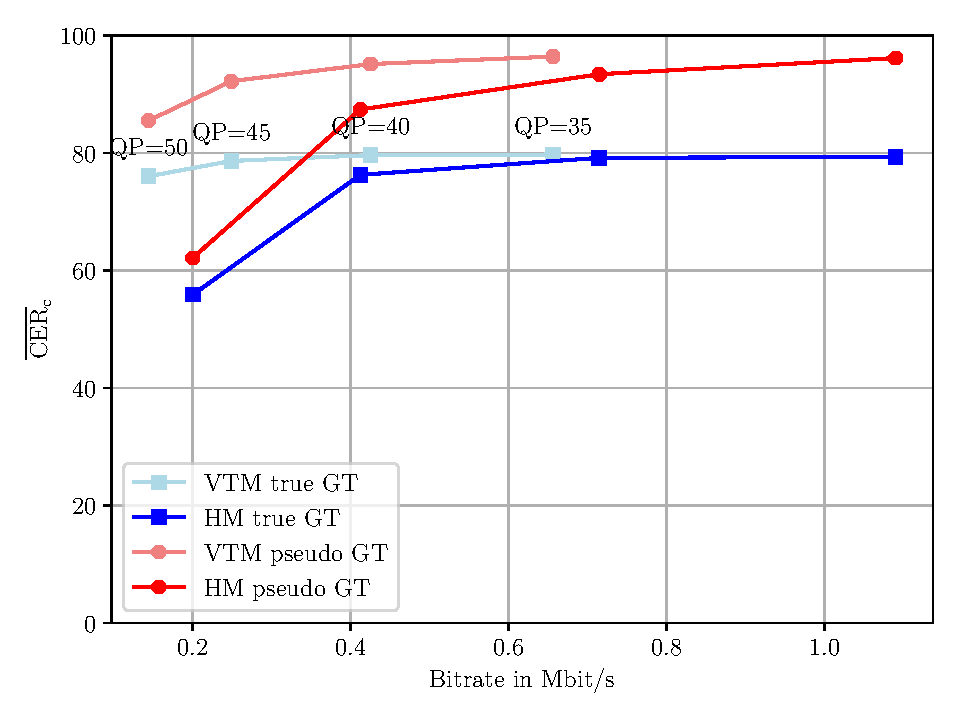
\includegraphics[width=\textwidth]{../images/analyze/codec_cer_size_ezocr_default.pdf}
    \caption{Comparison of $CER_{comp}$ and size for HM and VTM codec with default configuration for EasyOCR}
    \label{fig:codec_cer_size_ezocr_default}
\end{figure}

In \autoref{fig:codec_cer_size_ezocr_default} we can see the $CER_{comp}$ with regard to the pseudo and the true \gls{gt} against the size of the images for the HM and VTM codec with the default configuration for EasyOCR.
We can observe that the VTM curves are generally further to the top left corner, compared to the HM curves.
This means that the \gls{ocr} algorithm performs better on the VTM encoded images and they are smaller in size.
Additionally we can see that the trends of the true \gls{gt} curve pair (blue) are similar to the trends of the pseudo \gls{gt} curve pair (red).
To quantify this, we can calculate the \gls{bdrate} between these curves.

\begin{figure}[h]
    \centering
    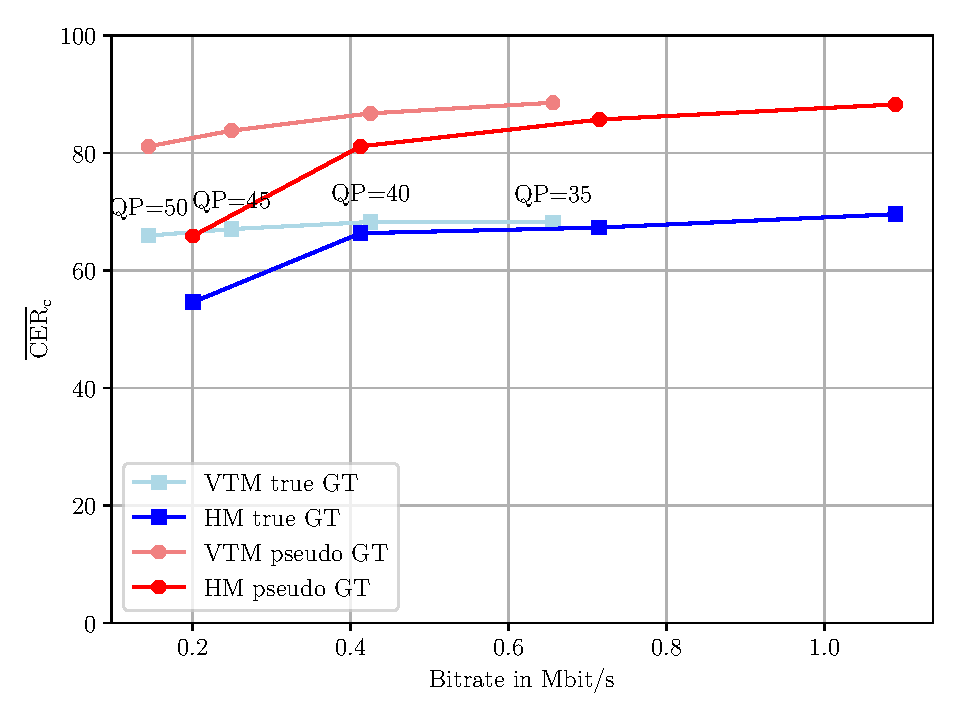
\includegraphics[width=\textwidth]{../images/analyze/codec_cer_size_tess_default.pdf}
    \caption{Comparison of $CER_{comp}$ and size for HM and VTM codec with default configuration for Tesseract \gls{ocr}}
    \label{fig:codec_cer_size_tess_default}
\end{figure}

In \autoref{fig:codec_cer_size_tess_default} we can see the $CER_{comp}$ with regard to the pseudo and the true \gls{gt} against the size of the images for the HM and VTM codec with the default configuration for Tesseract.
We can again observe that the VTM curves are generally further to top left, compared to the HM curves.
One exception is the \gls{qp} 35, where the VTM codec has a slightly worse $\text{CER}_{\text{c}}$ than the HM codec.
When comparing the two blue curves with the two red curves, it is difficult to see any other similarities.
Especially since the slope of the blue VTM curve is changing after every data point.
In this case we cannot calculate a \gls{bdrate} between the curves, since one of the curves is not monotonically increasing or decreasing.
However, we can clearly see that the pseudo \gls{gt} might not be the best alternative to compare codecs.


\begin{figure}[h]
    \centering
    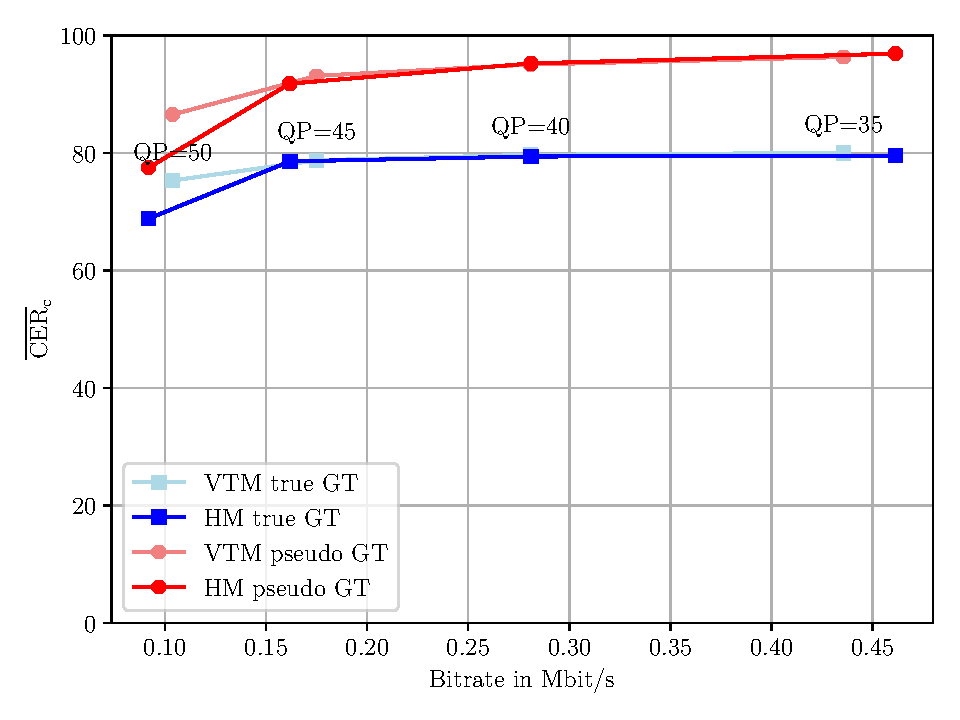
\includegraphics[width=\textwidth]{../images/analyze/codec_cer_size_ezocr_scc.pdf}
    \caption{Comparison of $CER_{comp}$ and size for HM and VTM codec with \gls{scc} configuration for EasyOCR}
    \label{fig:codec_cer_size_ezocr_scc}
\end{figure}

In \autoref{fig:codec_cer_size_ezocr_scc} we can see the $CER_{comp}$ with regard to the pseudo and the true \gls{gt} against the size of the images for the HM and VTM codec with the \gls{scc} configuration for EasyOCR.
The \gls{scc} configuration makes the HM codec perform very similarly to the VTM codec, with the exception of the \gls{qp} 50, where the VTM performs better again.
When comparing the blue and red curves, we can see that the trends are very similar.


\begin{figure}[h]
    \centering
    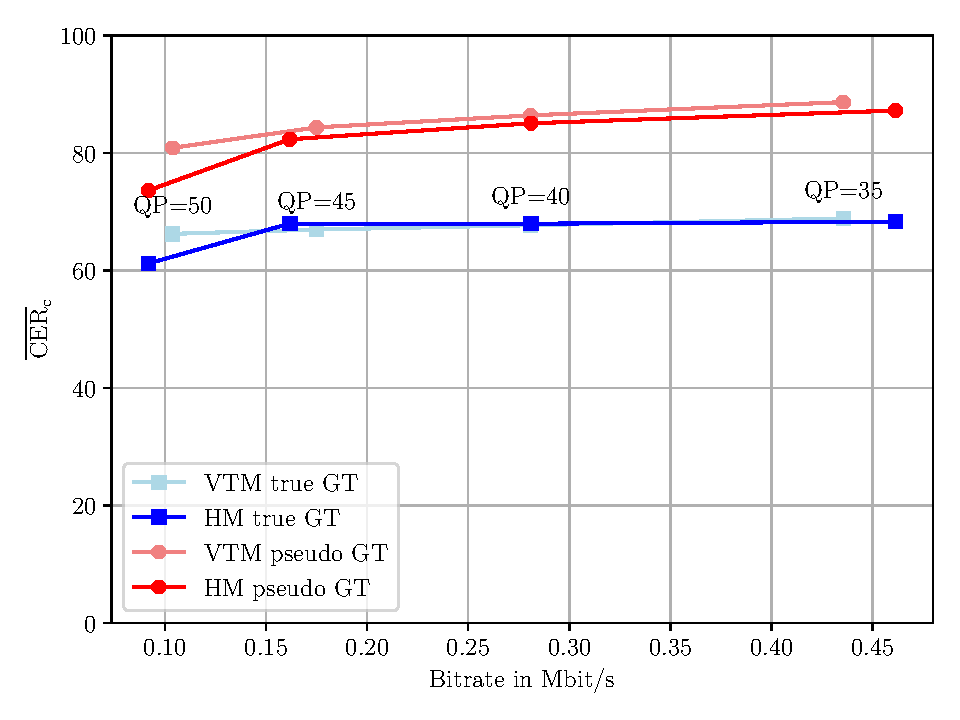
\includegraphics[width=\textwidth]{../images/analyze/codec_cer_size_tess_scc.pdf}
    \caption{Comparison of $CER_{comp}$ and size for HM and VTM codec with \gls{scc} configuration for Tesseract \gls{ocr}}
    \label{fig:codec_cer_size_tess_scc}
\end{figure}

In \autoref{fig:codec_cer_size_tess_scc} we can see the $CER_{comp}$ with regard to the pseudo and the true \gls{gt} against the size of the images for the HM and VTM codec with the \gls{scc} configuration for Tesseract.
The \gls{scc} configuration makes the HM codec perform very similarly to the VTM codec, with the exception of the \gls{qp} 50, where the VTM performs better, but only for the pseudo \gls{gt}.
When comparing the blue and red curves, we can see that the trends are not similar.
For the true \gls{gt}, the HM codec performs better than the VTM codec, while for the pseudo \gls{gt} the VTM codec performs better than the HM codec.

\begin{table}[h]
    \centering
    \begin{tabular}{|cc|cc|c|}
        \hline
        % algo, config, pseudo, true, diff
        \gls{ocr} Algorithm & Codec Configuration & Pseudo GT & True GT & Difference \\
        \hline
        \hline
        EasyOCR & Default & -59.28 & -61.02 & 1.73 \\
        EasyOCR & \gls{scc} & -7.41 & -1.1 & -6.32 \\
        \hline
        Tesseract & Default & -56.45 & --- & --- \\
        Tesseract & \gls{scc} & -19.57 & --- & --- \\
        \hline
    \end{tabular}
    \caption{Comparison of $\Delta R$ in \% between the pseudo and the true \gls{gt} for the different \gls{ocr} algorithms and codec configurations}
    \label{tab:bd_rate}
\end{table}

From \autoref{tab:bd_rate} we can see that the \gls{bdrate} way higher for the default configuration than for the \gls{scc} configuration for both the pseudo and the true \gls{gt}.
This reflects the large average distance of the curves seen in \autoref{fig:codec_cer_size_ezocr_default} and \autoref{fig:codec_cer_size_tess_default}, compared to the almost non existent distance seen in \autoref{fig:codec_cer_size_ezocr_scc} and \autoref{fig:codec_cer_size_tess_scc}.
For Tesseract \gls{ocr} we could not calculate the $\Delta R$ for the true \gls{gt}, since the curves are not monotonically increasing.
The difference between the pseudo and the true \gls{gt} is low with $1.73\%$ for the default configuration, but relatively high with $-6.31\%$ for the \gls{scc} configuration.
We can conclude that for images encoded with the default configurations of the HM and VTM codecs, EasyOCR can produce a good pseudo \gls{gt}.
- why not Tesseract? might have a decent bdrate but the curves are not monotonically increasing

To summarize, we can see that the \gls{ocr} algorithms perform better on the VTM encoded images than on the HM encoded images.
Additionally, the \gls{scc} configuration makes the HM codec perform very similarly to the VTM codec.
For the default configuration, EasyOCR seems to be a good pseudo \gls{gt}.
In contrast, Tesseract \gls{ocr} is not suitable for creating a pseudo \gls{gt}.
